\documentclass[a4paper, 12pt, oneside]{report}

% === Encodage et langue ===
\usepackage[utf8]{inputenc}
\usepackage[T1]{fontenc}
\usepackage[french]{babel}

% === Mise en page ===
\usepackage{geometry}
\geometry{left=2.5cm, right=2.5cm, top=2.5cm, bottom=2.5cm}
\usepackage{setspace}
\onehalfspacing

% === Graphiques et figures ===
\usepackage{graphicx}
\usepackage{float}
\usepackage{caption}
\usepackage{subcaption}
\usepackage{tikz}
\usetikzlibrary{positioning, shapes.geometric, arrows.meta, fit, calc}
\usepackage{pgfplots}
\pgfplotsset{compat=1.18}

% === Tableaux ===
\usepackage{booktabs}
\usepackage{longtable}
\usepackage{tabularx}
\usepackage{multirow}
\usepackage{array}
\usepackage{colortbl}

% === Mathématiques ===
\usepackage{amsmath, amssymb, amsthm}

% === Code source ===
\usepackage{listings}
\usepackage{xcolor}

% === En-têtes et pieds de page ===
\usepackage{fancyhdr}
\pagestyle{fancy}
\fancyhf{}
\fancyhead[L]{\nouppercase{\leftmark}}
\fancyhead[R]{\thepage}
\renewcommand{\headrulewidth}{0.4pt}
\fancypagestyle{plain}{
  \fancyhf{}
  \fancyhead[R]{\thepage}
  \renewcommand{\headrulewidth}{0pt}
}

% === Références et hyperliens ===
\usepackage{hyperref}
\hypersetup{
    colorlinks=true,
    linkcolor=blue!60!black,
    citecolor=green!50!black,
    urlcolor=blue,
    pdftitle={Analyse de données médicales massives pour la prédiction des MCV},
    pdfauthor={Naim Benjedou},
}

% === Bibliographie ===
\usepackage[backend=biber, style=numeric, sorting=nyt, maxbibnames=99]{biblatex}
\addbibresource{references.bib}

% === Couleurs personnalisées ===
\definecolor{codegreen}{rgb}{0,0.6,0}
\definecolor{codegray}{rgb}{0.5,0.5,0.5}
\definecolor{codepurple}{rgb}{0.45,0,0.75}
\definecolor{backcolour}{rgb}{0.96,0.96,0.94}
\definecolor{primary}{RGB}{31, 73, 125}
\definecolor{accent}{RGB}{192, 0, 0}

% === Style de listing Python ===
\lstdefinestyle{pythonstyle}{
    backgroundcolor=\color{backcolour},
    commentstyle=\color{codegreen}\itshape,
    keywordstyle=\color{codepurple}\bfseries,
    numberstyle=\tiny\color{codegray},
    stringstyle=\color{codegreen},
    basicstyle=\ttfamily\footnotesize,
    breakatwhitespace=false,
    breaklines=true,
    captionpos=b,
    keepspaces=true,
    numbers=left,
    numbersep=5pt,
    showspaces=false,
    showstringspaces=false,
    showtabs=false,
    tabsize=4,
    frame=single,
    rulecolor=\color{gray!40},
    language=Python
}
\lstset{style=pythonstyle}

% === Commandes personnalisées ===
\newcommand{\metric}[1]{\textbf{\textcolor{primary}{#1}}}
\newcommand{\todo}[1]{\textcolor{accent}{\textbf{[TODO: #1]}}}

% ============================================================
\begin{document}

% Page de garde
\begin{titlepage}
\thispagestyle{empty}

\begin{center}

% ───────────────── HEADER ─────────────────
\begin{minipage}[t]{0.32\textwidth}
\raggedright
\small
République Tunisienne\\
Ministère de l'Enseignement\\
Supérieur et de la Recherche\\
Scientifique

\vspace{0.1cm}
\rule{2.5cm}{0.4pt}

\vspace{0.1cm}

Université de Gafsa\\
Institut Supérieur des Sciences\\
Appliquées et de Technologie\\
de Gafsa
\end{minipage}
\hfill
\begin{minipage}[t]{0.28\textwidth}
\centering
\includegraphics[width=2.3cm]{figures/40740c82-2e26-4178-bf35-c7f001b6e764.jpeg}\\[0.15cm]
\includegraphics[width=1.8cm]{figures/43151050-7e39-4248-a071-b25d81e3094d.jpeg}
\end{minipage}
\hfill
\begin{minipage}[t]{0.32\textwidth}
\raggedleft
\small
Cycle de Formation en Mastère\\
professionnel\\
dans la discipline\\
............................

\vspace{0.1cm}
\rule{2.5cm}{0.4pt}

\vspace{0.1cm}

\textbf{Mémoire de MASTÈRE}\\
D'ordre : 2025 -- ESC
\end{minipage}

\vspace{0.2cm}

\color{blue}
\rule{\textwidth}{1pt}
\color{black}

\vspace{0.2cm}

% ───────────────── TITRE ─────────────────
{\fontsize{22}{24}\selectfont \textbf{MEMOIRE}}

\vspace{0.3cm}

\small
\textit{Présenté à}\\[0.15cm]
L'Institut Supérieur des Sciences Appliquées et de Technologie de Gafsa

\vspace{0.3cm}

Département : Informatique

\vspace{0.3cm}

\textit{En vue de l'obtention du diplôme de}

\vspace{0.3cm}

{\Large \textbf{MASTÈRE PROFESSIONNEL}}
\vspace{0.3cm}
\begin{flushleft}
\hspace{2cm}\textbf{Mention :} \dotfill
\end{flushleft}

\vspace{-0.1cm}

\begin{flushleft}
\hspace{2cm}\textbf{Spécialité :} Sciences des données
\end{flushleft}

\vspace{0.2cm}

\textit{Par :}\\[0.1cm]
{\large \textbf{Marwa ABADA}}

\vspace{0.2cm}

\rule{7cm}{0.8pt}

\vspace{0.2cm}

{\normalsize \bfseries
Analyse de données médicales massives pour la prédiction\\[0.15cm]
des maladies cardiovasculaires à l'aide d'Apache Spark\\[0.15cm]
et des réseaux de neurones profonds
}

\vspace{0.2cm}

\rule{7cm}{0.8pt}

\vspace{0.2cm}

\small
Soutenu le .../.../2025 devant le jury composé de :

\vspace{0.3cm}

\begin{tabular}{p{7.5cm}p{3.5cm}}
M. ........................................ & Président \\
M. ........................................ & Rapporteur \\
M. ........................................ & Encadrant \\
\end{tabular}

\vfill

{\large \textbf{A.U : 2024 -- 2025}}

\end{center}
\end{titlepage}

% ─────────────────────────────────────────────────────────────────────────────
% DÉDICACE
% ─────────────────────────────────────────────────────────────────────────────
\thispagestyle{empty}
\null\vfill
\begin{center}
  {\color{black}\rule{0.6\textwidth}{1pt}}\\[1cm]
  {\Large\itshape\bfseries Dédicace}\\[1cm]
  {\color{black}\rule{0.6\textwidth}{0.4pt}}
\end{center}
\vspace{1cm}

\begin{center}
\begin{minipage}{0.75\textwidth}
\setlength{\parindent}{0pt}
\setlength{\parskip}{0.8em}
\itshape

À mes très chers parents,\\
pour leur amour inconditionnel, leurs sacrifices constants\\
et leur soutien indéfectible tout au long de mon parcours.\\
Ce travail est le fruit de votre confiance en moi.

À ma famille,\\
dont l'encouragement et la chaleur ont été ma force\\
dans les moments les plus difficiles.

À mes amis et à tous ceux qui ont contribué,\\
de près ou de loin, à l'accomplissement de ce projet.

\vspace{1em}
\begin{flushright}
\textbf{Marwa Abada}
\end{flushright}
\end{minipage}
\end{center}

\vfill\null
\newpage

% ─────────────────────────────────────────────────────────────────────────────
% REMERCIEMENTS
% ─────────────────────────────────────────────────────────────────────────────
\thispagestyle{empty}
\begin{center}
  {\Large\bfseries Remerciements}\\[0.6cm]
\end{center}
\vspace{0.8cm}

Au terme de ce travail, il m'est particulièrement agréable d'exprimer ma
gratitude et mes sincères remerciements à toutes les personnes qui ont
contribué, de près ou de loin, à la réalisation de ce projet.

Je tiens tout d'abord à adresser mes plus vifs remerciements à
\textbf{Mme Thouraya Gouasmi}, mon encadrante, pour son accompagnement,
sa disponibilité, ses précieux conseils ainsi que son soutien tout au long
de cette expérience. Ses orientations techniques et pédagogiques ont été
d'une grande importance dans la réussite de ce projet.

J'exprime également ma profonde reconnaissance à l'ensemble des enseignants
et du personnel de \textbf{L'Institut Supérieur des Sciences Appliquées et de Technologie de Gafsa},
pour la qualité de la formation dispensée ainsi que pour les connaissances
acquises durant mon parcours universitaire.

Je remercie chaleureusement l'administration et toute l'équipe de
l'institut pour l'accueil, l'encadrement et les conditions favorables
offertes durant la période de stage.

Mes sincères remerciements vont également à ma famille et à mes proches
pour leur soutien moral, leurs encouragements constants et leur confiance
tout au long de mon parcours académique.

Enfin, je remercie toutes les personnes qui ont contribué, directement ou
indirectement, à l'aboutissement de ce travail.

\vspace{1cm}
\begin{flushright}
\itshape Marwa Abada\\
Gafsa, 2026
\end{flushright}

\newpage

% ─────────────────────────────────────────────────────────────────────────────
% RÉSUMÉ
% ─────────────────────────────────────────────────────────────────────────────
\chapter*{Résumé}
\addcontentsline{toc}{chapter}{Résumé}

Ce mémoire présente un pipeline Big Data end-to-end pour la prédiction des maladies cardiovasculaires (MCV) à partir du \textit{Behavioral Risk Factor Surveillance System} (BRFSS) 2020--2024, comptant plus de 2,17 millions d'enregistrements épidémiologiques américains.

Le pipeline traite 2\,176\,776 enregistrements BRFSS bruts avec Apache Spark (PySpark)~: déduplication de 416\,535 lignes, binarisation des codes BRFSS non standards, et imputation des valeurs manquantes. Un feature engineering multi-méthodes (corrélations de Pearson et Spearman, importance Gini, test du $\chi^2$) sélectionne 15 variables parmi lesquelles deux features dérivées composites, RiskScore et HealthIndex. Deux modèles sont entraînés sur un partitionnement stratifié 70/15/15~: un réseau de neurones profond à architecture 256-128-64 (TensorFlow~2.19) et XGBoost~3.2 avec \textit{RandomizedSearchCV} sur 20 combinaisons de paramètres.

Les deux modèles convergent vers une AUC-ROC de 0,819 (DNN~: 0,8191, XGBoost~: 0,8195). Le DNN, avec un seuil de décision optimisé à 0,6713 par courbe Précision-Rappel, obtient une accuracy de 82,25~\% et un recall de 56,3~\% sur la classe positive. XGBoost, avec 400 arbres et un \textit{scale\_pos\_weight} de 8,69, atteint un recall de 79,9~\%. Le benchmark sur cinq fractions croissantes du jeu d'entraînement montre qu'XGBoost standalone est 36 à 97 fois plus rapide que Spark~GBT en mode local~; l'apport de Spark dans ce pipeline est donc concentré sur l'étape de preprocessing distribué.

Un tableau de bord interactif Streamlit a été développé pour visualiser l'ensemble des résultats.

\vspace{0.4cm}
\textbf{Mots-clés :} Maladies cardiovasculaires, Big Data, Apache Spark, Deep Learning, XGBoost, BRFSS, Classification binaire, Déséquilibre de classes.

\newpage

% ─────────────────────────────────────────────────────────────────────────────
% ABSTRACT
% ─────────────────────────────────────────────────────────────────────────────
\chapter*{Abstract}
\addcontentsline{toc}{chapter}{Abstract}

This thesis presents an end-to-end Big Data pipeline for cardiovascular disease (CVD) prediction using the Behavioral Risk Factor Surveillance System (BRFSS) 2020--2024 dataset, comprising over 2.17 million epidemiological records.

The work is organized around five main axes: (1) data ingestion and cleaning with Apache Spark, processing 2.17 million rows and removing 416,535 duplicates; (2) feature engineering including Pearson/Spearman correlation analysis, Gini importance, chi-squared testing, and creation of derived features (RiskScore, HealthIndex); (3) training a Deep Neural Network (DNN) with a 256-128-64 architecture and class-weight-based imbalance handling; (4) training and optimizing XGBoost via RandomizedSearchCV; and (5) a performance benchmark between XGBoost standalone and Spark GBTClassifier across increasing dataset fractions.

Results show that both models achieve comparable AUC-ROC: 0.8191 for the DNN and 0.8195 for XGBoost. Using a threshold optimized at 0.6713 via the Precision-Recall curve, the DNN achieves 82.25\% accuracy and 56.3\% recall on the positive class. XGBoost, with 400 trees and a \textit{scale\_pos\_weight} of 8.69, reaches 79.9\% recall. The benchmark demonstrates that XGBoost standalone is 36 to 97 times faster than Spark GBT in local single-machine mode, highlighting that Spark's contribution lies in distributed preprocessing rather than model training. An interactive Streamlit dashboard was developed to visualize all results.

\vspace{0.4cm}
\textbf{Keywords:} Cardiovascular diseases, Big Data, Apache Spark, Deep Learning, XGBoost, BRFSS, Binary classification, Class imbalance.

\newpage


% Numérotation romaine pour les pages préliminaires
\pagenumbering{roman}
\setcounter{page}{1}

% Table des matières
\tableofcontents
\newpage

% Liste des figures
\listoffigures
\addcontentsline{toc}{chapter}{Liste des figures}
\newpage

% Liste des tableaux
\listoftables
\addcontentsline{toc}{chapter}{Liste des tableaux}
\newpage

% Numérotation arabe pour le corps du document
\pagenumbering{arabic}
\setcounter{page}{1}

% Chapitres principaux
\chapter{Introduction générale}

\section{Contexte général}

Les maladies cardiovasculaires (MCV) sont la première cause de mortalité dans le monde~:
selon l'Organisation Mondiale de la Santé, elles causent 17,9 millions de décès par an,
soit 31~\% de la mortalité mondiale \cite{who2023}.
Plus de trois quarts de ces décès surviennent dans les pays à revenu faible
ou intermédiaire, où les programmes de prévention restent insuffisants.

La détection précoce du risque cardiovasculaire est une priorité de santé publique.
Un dépistage en amont des événements cardiaques permet de concentrer les interventions
préventives sur les populations les plus exposées et de limiter les hospitalisations
évitables. Les facteurs de risque modifiables des MCV sont bien documentés dans la
littérature épidémiologique~: hypertension artérielle, hypercholestérolémie, diabète,
tabagisme, obésité, sédentarité et consommation excessive d'alcool \cite{roth2020}.

Les techniques de machine learning appliquées aux grandes enquêtes épidémiologiques
offrent une voie pour exploiter ces facteurs à l'échelle de la population.
Le \textit{Behavioral Risk Factor Surveillance System} (BRFSS), coordonné par les
Centers for Disease Control and Prevention (CDC) américains, produit chaque année
400\,000 à 500\,000 réponses couvrant des centaines de variables comportementales
et médicales. La version poolée 2020--2024 dépasse les 2 millions d'enregistrements
et nécessite des outils de traitement distribué pour être exploitée efficacement.

\section{Problématique}

Comment exploiter des données épidémiologiques massives, dépassant les 2 millions d'enregistrements, pour prédire le risque de maladie cardiovasculaire, et comment comparer de façon rigoureuse une approche Deep Learning et une approche de Machine Learning classique sur ce type de données ?

Cette problématique soulève plusieurs défis techniques et méthodologiques :

\begin{enumerate}
    \item \textbf{Le volume de données :} Le dataset BRFSS 2020--2024 poolé contient 2 176 776 enregistrements, ce qui dépasse les capacités de traitement des outils classiques en mémoire vive. Des outils de traitement distribué comme Apache Spark sont nécessaires pour ingérer, nettoyer et préparer ces données efficacement.

    \item \textbf{Le déséquilibre de classes :} Avec une prévalence de MCV d'environ 10,3\% dans le dataset, les modèles standards tendent à classifier l'ensemble des observations comme négatif pour maximiser l'accuracy. Des techniques spécifiques de gestion du déséquilibre sont nécessaires.

    \item \textbf{La qualité et l'encodage des données :} Le BRFSS utilise des conventions d'encodage non standards (1 = Oui, 2 = Non pour les variables binaires), nécessitant une phase de binarisation rigoureuse avant toute modélisation.

    \item \textbf{La comparaison rigoureuse des modèles :} Comparer un DNN et XGBoost requiert un protocole d'évaluation complet : mêmes données de test, mêmes métriques, optimisation du seuil de classification, et analyse de la capacité de détection de la classe positive.

    \item \textbf{L'apport réel d'Apache Spark :} Quantifier objectivement la valeur ajoutée de Spark en mode local versus une approche standalone nécessite un benchmark contrôlé sur des fractions croissantes du jeu de données.
\end{enumerate}

\section{Objectifs du projet}

\subsection{Objectif principal}

Concevoir et implémenter un pipeline Big Data end-to-end, capable d'ingérer, prétraiter, modéliser et évaluer les données BRFSS 2020--2024 pour prédire le risque de maladie cardiovasculaire, avec une comparaison quantitative entre XGBoost et un réseau de neurones profond.

\subsection{Objectifs secondaires}

\begin{enumerate}
    \item \textbf{Traitement distribué :} Démontrer la faisabilité et les performances d'Apache Spark pour le chargement et le prétraitement de données épidémiologiques massives (>2M lignes).

    \item \textbf{Feature engineering avancé :} Construire un ensemble de features discriminantes à partir de 14 variables BRFSS brutes, incluant la création de features dérivées composite (RiskScore, HealthIndex).

    \item \textbf{Modélisation comparative :} Entraîner, optimiser et comparer un DNN (TensorFlow/Keras) et XGBoost sur les mêmes données, avec gestion explicite du déséquilibre de classes et optimisation du seuil de décision.

    \item \textbf{Benchmark de performance :} Évaluer quantitativement le temps d'entraînement de Spark GBTClassifier versus XGBoost standalone sur des fractions croissantes du dataset.

    \item \textbf{Visualisation :} Développer un tableau de bord interactif Streamlit pour présenter les résultats de manière accessible.
\end{enumerate}

\section{Contributions}

Les principales contributions de ce travail sont :

\begin{itemize}
    \item Un pipeline de binarisation spécifique au format BRFSS, gérant les encodages non standards (1=Oui/2=Non) et la variable dérivée \texttt{\_MICHD} pour la cible cardiovasculaire.
    \item Un benchmark contrôlé Spark vs. XGBoost standalone sur 5 fractions de données (10\% à 100\%, soit 149\,510 à 1\,495\,609 lignes).
    \item Une analyse de l'impact du seuil de décision sur le compromis précision/rappel en présence d'un déséquilibre de classes 9:1.
    \item Un tableau de bord Streamlit en 3 pages (EDA interactive, Résultats des modèles, Impact Spark) fonctionnant sans infrastructure Big Data.
\end{itemize}

\section{Organisation du rapport}

Ce mémoire est organisé en six chapitres :

\begin{description}
    \item[\textbf{Chapitre 2 — État de l'art}] Revue de la littérature sur la prédiction des MCV, les techniques de machine learning sur données médicales déséquilibrées, et les approches Big Data pour les enquêtes épidémiologiques.

    \item[\textbf{Chapitre 3 — Méthodologie}] Description du dataset BRFSS, du pipeline de traitement, des architectures de modèles choisies et du protocole d'évaluation.

    \item[\textbf{Chapitre 4 — Implémentation}] Détails techniques de l'environnement de développement, du code PySpark, de l'architecture DNN et de la configuration XGBoost.

    \item[\textbf{Chapitre 5 — Résultats et Discussion}] Présentation et analyse des résultats expérimentaux : EDA, performances des modèles, benchmark Spark, comparaison avec les critères de succès et avec la littérature.

    \item[\textbf{Chapitre 6 — Conclusion et Perspectives}] Synthèse des apports du travail, limites identifiées et pistes d'amélioration futures.
\end{description}

\chapter{État de l'art}

\section{Les maladies cardiovasculaires}

\subsection{Définition et épidémiologie}

Les maladies cardiovasculaires (MCV) désignent un groupe de pathologies affectant le cœur et les vaisseaux sanguins. Elles comprennent notamment les cardiopathies coronariennes (angine de poitrine, infarctus du myocarde), les accidents vasculaires cérébraux (AVC), l'insuffisance cardiaque, et les artériopathies périphériques. Selon l'OMS, les MCV causent 17,9 millions de décès annuels \cite{who2023}, dont 85\% sont imputables aux cardiopathies coronariennes et aux AVC.

En termes de fardeau économique, les MCV coûtent aux États-Unis plus de 363 milliards de dollars par an en dépenses de santé et pertes de productivité \cite{virani2021}. La prévention primaire et secondaire, par la détection précoce des facteurs de risque, représente le levier le plus efficace pour réduire ce fardeau.

\subsection{Facteurs de risque identifiés}

La littérature épidémiologique distingue deux catégories de facteurs de risque cardiovasculaire \cite{roth2020} :

\begin{itemize}
    \item \textbf{Facteurs non modifiables} : âge, sexe masculin, antécédents familiaux de MCV, origine ethnique.
    \item \textbf{Facteurs modifiables} :
    \begin{itemize}
        \item \textit{Comportementaux} : tabagisme, sédentarité, alimentation déséquilibrée, consommation excessive d'alcool.
        \item \textit{Médicaux} : hypertension artérielle, hypercholestérolémie, diabète de type 2, obésité (IMC $>$ 30).
        \item \textit{Psychosociaux} : stress chronique, santé mentale dégradée.
    \end{itemize}
\end{itemize}

Les scores de risque cardiovasculaire traditionnels, tels que le score de Framingham \cite{wilson1998} ou le score SCORE2 européen \cite{score2}, agrègent ces facteurs de risque en une probabilité d'événement cardiovasculaire à 10 ans. Ces scores ont cependant des limites : ils ont été développés sur des populations spécifiques, ne capturent pas les interactions non linéaires entre variables, et n'exploitent pas pleinement la richesse des enquêtes populationnelles à grande échelle.

\section{Le dataset BRFSS}

\subsection{Présentation de l'enquête}

Le \textit{Behavioral Risk Factor Surveillance System} (BRFSS) est la plus grande enquête téléphonique de santé au monde, coordonnée par les Centers for Disease Control and Prevention (CDC) des États-Unis \cite{cdc_brfss}. Menée annuellement depuis 1984 dans les 50 États américains, elle collecte des données sur les comportements à risque, les conditions chroniques et l'utilisation des services de santé préventifs.

Chaque édition annuelle recueille entre 400\,000 et 500\,000 réponses, avec des questionnaires comprenant des centaines de variables (modules de base, modules optionnels, modules spécifiques aux États). La version poolée 2020--2024 utilisée dans ce projet comptabilise 2\,176\,776 enregistrements bruts avant nettoyage.

\subsection{Variable cible : HeartDiseaseorAttack}

La variable cible utilisée dans ce travail est dérivée de la variable BRFSS \texttt{\_MICHD} (Respondents that have ever reported having coronary heart disease or myocardial infarction). Cette variable composite est définie comme :

$$\texttt{\_MICHD} = 1 \text{ si cardiopathie coronarienne OU infarctus du myocarde}$$

La transformation appliquée est :
\begin{align*}
    \texttt{HeartDiseaseorAttack} &= 1 \text{ si } \texttt{\_MICHD} = 1 \text{ (oui)} \\
    \texttt{HeartDiseaseorAttack} &= 0 \text{ si } \texttt{\_MICHD} = 2 \text{ (non)}
\end{align*}

Le taux de prévalence résultant est de 10,32\% dans le dataset nettoyé, contre environ 5--6\% si l'on utilisait uniquement la variable d'infarctus du myocarde.

\section{Techniques de Machine Learning pour la prédiction des MCV}

\subsection{Arbres de décision et méthodes d'ensemble}

Les méthodes d'ensemble, notamment les forêts aléatoires (\textit{Random Forest}) et le boosting de gradient, ont démontré des performances supérieures aux modèles linéaires pour la prédiction des MCV sur des données BRFSS.

Nickels et al. \cite{nickels2023} ont appliqué un Random Forest sur le BRFSS 2020, atteignant une AUC de 0,912 avec 18 variables cliniques incluant l'hypertension et l'hypercholestérolémie. Cette performance supérieure aux nôtres s'explique en partie par la disponibilité dans leur jeu de données de variables comme HighBP et HighChol, absentes du fichier poolé ML utilisé dans notre étude.

Mesdaghinia et al. \cite{mesdaghinia2023} ont obtenu une AUC de 0,872 avec XGBoost sur le BRFSS 2019, en incluant 23 variables. Leur approche utilisait la technique SMOTE (\textit{Synthetic Minority Oversampling Technique}) pour gérer le déséquilibre de classes. Notre approche, fondée sur les class weights, présente l'avantage de ne pas créer de données synthétiques et de préserver les distributions originales.

\subsection{XGBoost}

XGBoost (\textit{eXtreme Gradient Boosting}) \cite{chen_xgboost} est un algorithme d'ensemble basé sur le boosting de gradient qui a révolutionné les compétitions de machine learning depuis son introduction en 2016. Son principe repose sur la construction itérative d'arbres de décision, chaque arbre corrigeant les erreurs du précédent par descente de gradient sur une fonction de perte différentiable.

Les avantages d'XGBoost pour notre cas d'usage incluent :
\begin{itemize}
    \item Le paramètre \texttt{scale\_pos\_weight} qui permet de pondérer la classe positive sans sur-échantillonnage.
    \item La régularisation L1/L2 intégrée qui prévient le sur-apprentissage.
    \item La gestion native des valeurs manquantes par apprentissage de la direction de branchement optimale.
    \item La parallélisation native du calcul au niveau des arbres et des splits.
\end{itemize}

\subsection{Réseaux de neurones profonds (DNN)}

Les réseaux de neurones profonds (\textit{Deep Neural Networks}) permettent d'apprendre des représentations hiérarchiques non linéaires des données. Pour les données tabulaires médicales, les architectures à couches entièrement connectées (\textit{fully connected}) constituent généralement le premier choix \cite{shwartz2022}.

Patel et al. \cite{patel2023} ont obtenu un F1-score de 0,834 sur le BRFSS 2021 en combinant un DNN avec SMOTE. Kumar et al. \cite{kumar2023} ont utilisé des réseaux LSTM pour capturer la dimension longitudinale des données BRFSS, atteignant une AUC de 0,891. Dans notre contexte non longitudinal, un DNN feed-forward avec BatchNormalization et Dropout représente une architecture adaptée.

La gestion du déséquilibre dans les DNN se fait par le mécanisme de \textit{class weights} : la fonction de perte (Binary Crossentropy) est pondérée inversement proportionnellement à la fréquence de chaque classe :

$$w_k = \frac{N_{total}}{n_{classes} \times N_k}$$

Dans notre cas : $w_0 = 0,558$ (classe négative) et $w_1 = 4,847$ (classe positive), reflétant un rapport de déséquilibre de 9:1.

\subsection{Optimisation du seuil de classification}

La plupart des études utilisent le seuil par défaut de 0,5 pour la classification binaire. Cette approche est inadaptée en présence de déséquilibre de classes. La courbe Précision-Rappel (PR curve) permet d'identifier le seuil qui maximise le F1-score \cite{davis2006} :

$$F_1 = 2 \cdot \frac{\text{Précision} \times \text{Rappel}}{\text{Précision} + \text{Rappel}}$$

Cette analyse est particulièrement importante en contexte médical, où le compromis entre faux positifs (patients incorrectement alertés) et faux négatifs (patients à risque non détectés) a des implications cliniques directes. Dans notre étude, le seuil optimal identifié est de 0,6713 pour le DNN, contre le seuil naïf de 0,5.

\section{Big Data et Apache Spark pour les données médicales}

\subsection{Apache Spark}

Apache Spark est un framework open-source de traitement distribué de données massives, développé à l'Université de Californie à Berkeley et maintenu par la fondation Apache \cite{zaharia2016}. Son modèle de programmation fondé sur les \textit{Resilient Distributed Datasets} (RDD) et les DataFrames permet de traiter des volumes de données dépassant la mémoire vive d'une seule machine en distribuant le calcul sur un cluster de nœuds.

Les principales caractéristiques qui justifient son utilisation dans ce projet sont :
\begin{itemize}
    \item Le traitement en mémoire (\textit{in-memory computing}), offrant des performances 10 à 100 fois supérieures à Hadoop MapReduce pour les workloads itératifs.
    \item Le support natif du format Parquet, optimisé pour les opérations analytiques colonaires.
    \item La bibliothèque MLlib, offrant des implémentations distribuées d'algorithmes de ML classiques.
    \item L'API unifiée (Scala, Java, Python, R) permettant de réutiliser la même logique pour le preprocessing et l'entraînement.
\end{itemize}

Zhang et al. \cite{zhang2023} ont démontré qu'un pipeline Spark MLlib peut traiter 3 millions d'enregistrements BRFSS en moins de 4 minutes sur un cluster de 8 nœuds, avec un speedup quasi-linéaire en fonction du nombre de nœuds. En mode local (une seule machine), cependant, l'overhead du scheduler Spark et de la sérialisation des partitions peut annuler cet avantage pour les petits et moyens volumes.

\subsection{Spark MLlib --- GBTClassifier}

La classe \texttt{GBTClassifier} de Spark MLlib implémente les arbres de gradient boostés de manière distribuée. Chaque arbre est construit en partitionnant les données sur l'ensemble des nœuds du cluster, permettant de traiter des datasets ne tenant pas en mémoire sur une seule machine. Cependant, la sérialisation des modèles et la synchronisation inter-nœuds introduisent un overhead significatif par rapport à XGBoost en mode local.

\subsection{Comparaison Spark vs. standalone en mode local}

La littérature établit clairement que Spark est avantageux pour les volumes dépassant plusieurs dizaines de millions de lignes sur un vrai cluster. Pour les volumes de l'ordre du million de lignes sur une machine locale, XGBoost avec parallélisation OpenMP offre généralement des temps d'entraînement significativement plus courts \cite{shwartz2022}. Notre benchmark quantifie cet écart sur les données BRFSS spécifiques à ce projet.

\section{Synthèse et positionnement}

\begin{table}[H]
\centering
\caption{Synthèse des travaux existants sur la prédiction des MCV avec BRFSS}
\label{tab:etat_art}
\begin{tabular}{p{3.5cm}p{1.5cm}p{3cm}p{1.5cm}p{3.5cm}}
\toprule
\textbf{Auteurs} & \textbf{Année} & \textbf{Méthode} & \textbf{AUC} & \textbf{Particularités} \\
\midrule
Nickels et al. \cite{nickels2023}    & 2023 & Random Forest       & 0,912 & 18 vars dont HighBP/HighChol \\
Mesdaghinia et al. \cite{mesdaghinia2023} & 2023 & XGBoost + SMOTE & 0,872 & 23 variables, BRFSS 2019 \\
Patel et al. \cite{patel2023}        & 2023 & DNN + SMOTE         & 0,834 & F1=0,834, BRFSS 2021 \\
Kumar et al. \cite{kumar2023}        & 2023 & LSTM                & 0,891 & Données longitudinales \\
Zhang et al. \cite{zhang2023}        & 2023 & Spark MLlib         & ---   & 3M lignes, cluster 8 nœuds \\
\midrule
\textbf{Ce travail}                  & 2026 & DNN + XGBoost + Spark & 0,820 & 2,17M lignes, pipeline E2E \\
\bottomrule
\end{tabular}
\end{table}

Ce travail se distingue des précédents sur plusieurs points. Il utilise le dataset poolé
2020--2024, le plus volumineux disponible publiquement sur Kaggle. Il intègre un benchmark
contrôlé Spark vs. XGBoost standalone dans le même pipeline, ce qu'aucun des travaux
cités ne fait. Il applique l'optimisation du seuil par courbe Précision-Rappel et délivre
un tableau de bord interactif. L'AUC obtenue (0,820) est inférieure aux meilleurs résultats
de la littérature~; cette différence s'explique par l'absence de HighBP et HighChol dans le
fichier poolé ML utilisé, deux variables qui contribuent fortement au pouvoir discriminant
dans les études de Nickels et al.\ et Mesdaghinia et al.

\chapter{Méthodologie}
\label{chap:methodologie}

\section{Description du dataset}

\subsection{Caractéristiques générales}

Le dataset BRFSS (\textit{Behavioral Risk Factor Surveillance System}) 2020--2024 poolé et préparé pour le machine learning présente les caractéristiques décrites dans le tableau \ref{tab:dataset_chars}.

\begin{table}[H]
\centering
\caption{Caractéristiques du dataset BRFSS 2020--2024}
\label{tab:dataset_chars}
\begin{tabular}{ll}
\toprule
\textbf{Caractéristique} & \textbf{Valeur} \\
\midrule
Nombre d'observations brutes & 2\,176\,776 \\
Doublons supprimés & 416\,535 \\
Nombre d'observations après nettoyage & 1\,760\,241 \\
Nombre de variables modélisées & 14 (+ 2 features dérivées) \\
Variable cible & \texttt{HeartDiseaseorAttack} (binaire, 0/1) \\
Prévalence MCV (classe positive) & 10,32\% \\
Format source & Parquet (fichier poolé \texttt{\_ml}) \\
\bottomrule
\end{tabular}
\end{table}

\subsection{Variables sélectionnées}

Les 14 variables retenues après sélection sont décrites dans le tableau \ref{tab:variables}. Ces variables ont été choisies parmi les 129 colonnes du dataset brut BRFSS sur la base de leur pertinence clinique documentée dans la littérature et de leur disponibilité dans le fichier poolé ML.

\begin{longtable}{p{3.8cm}p{4cm}p{2cm}p{3.5cm}}
\caption{Variables sélectionnées et leur encodage}
\label{tab:variables}\\
\toprule
\textbf{Variable} & \textbf{Description} & \textbf{Type} & \textbf{Encodage} \\
\midrule
\endfirsthead
\multicolumn{4}{c}{\textit{Suite du tableau \ref{tab:variables}}}\\
\toprule
\textbf{Variable} & \textbf{Description} & \textbf{Type} & \textbf{Encodage} \\
\midrule
\endhead
\bottomrule
\endlastfoot
\texttt{HeartDiseaseorAttack} & Maladie coronarienne ou IM & Binaire & 0=Non, 1=Oui \\
\texttt{BMI} & Indice de masse corporelle & Continu & \_BMI5 / 100 \\
\texttt{Smoker} & Tabagisme (100+ cigarettes/vie) & Binaire & 0=Non, 1=Oui \\
\texttt{Stroke} & Antécédent d'AVC & Binaire & 0=Non, 1=Oui \\
\texttt{Diabetes} & Diabète diagnostiqué & Binaire & 0=Non, 1=Oui \\
\texttt{PhysActivity} & Activité physique (30j) & Binaire & 0=Non, 1=Oui \\
\texttt{GenHlth} & Santé générale auto-évaluée & Ordinal & 1=Excellent à 5=Mauvaise \\
\texttt{MentHlth} & Jours santé mentale mauvaise & Discret & 0--30 jours (88→0) \\
\texttt{PhysHlth} & Jours santé physique mauvaise & Discret & 0--30 jours \\
\texttt{DiffWalk} & Difficultés à marcher & Binaire & 0=Non, 1=Oui \\
\texttt{Sex} & Sexe & Binaire & 0=Homme, 1=Femme \\
\texttt{Age} & Tranche d'âge BRFSS & Ordinal & 1 (18-24) à 13 (80+) \\
\texttt{Education} & Niveau d'éducation & Ordinal & 1 (aucune) à 6 (diplômé) \\
\texttt{HvyAlcoholConsump} & Consommation excessive d'alcool & Binaire & 0=Non, 1=Oui \\
\bottomrule
\end{longtable}

\subsection{Variables absentes du fichier poolé ML}

Une contrainte importante de ce travail est l'absence de quatre variables cliniquement importantes dans le fichier poolé ML disponible :

\begin{itemize}
    \item \texttt{HighBP} (hypertension artérielle) — remplacée par \texttt{Stroke} dans le calcul du RiskScore
    \item \texttt{HighChol} (hypercholestérolémie) — remplacée par \texttt{DiffWalk} dans le calcul du RiskScore
    \item \texttt{Income} (revenu du foyer) — absente du modèle
    \item \texttt{NoDocbcCost} (renoncement aux soins pour raisons financières) — absente du modèle
\end{itemize}

Ces variables, présentes dans le fichier EDA et abondamment utilisées dans la littérature (Nickels et al.\ obtiennent une AUC de 0,912 avec \texttt{HighBP}/\texttt{HighChol}), expliquent en partie le plateau d'AUC observé à 0,82 dans nos modèles. Cette limitation est d'ordre documentaire et non algorithmique.

% ─────────────────────────────────────────────────────────────────────────────
\section{Architecture du pipeline}
% ─────────────────────────────────────────────────────────────────────────────

Le pipeline développé dans ce projet suit une architecture séquentielle en cinq phases, représentée à la figure~\ref{fig:pipeline}. Chaque phase produit des artefacts persistants — fichiers au format Parquet, tableaux NumPy, fichiers JSON — qui constituent les entrées de la phase suivante, garantissant la reproductibilité de l'ensemble du processus et facilitant la reprise en cas d'interruption de session.

\begin{figure}[H]
\centering
\begin{tikzpicture}[
    box/.style={rectangle, draw=primary, fill=primary!10, rounded corners=5pt,
                minimum width=11cm, minimum height=1.1cm,
                text centered, font=\small\bfseries, text=primary!85!black},
    arr/.style={->, >=stealth, thick, color=primary}
]
    \node[box] at (0, 0)   (p1)
        {Phase 1 — Ingestion et nettoyage
         {\normalfont\scriptsize\itshape (PySpark, Parquet, binarisation BRFSS, déduplication)}};
    \node[box] at (0,-1.9) (p2)
        {Phase 2 — Analyse exploratoire et Feature Engineering
         {\normalfont\scriptsize\itshape (corrélation, Gini, $\chi^2$, ACP, features dérivées)}};
    \node[box] at (0,-3.8) (p3)
        {Phase 3 — Entraînement du réseau de neurones profond
         {\normalfont\scriptsize\itshape (TensorFlow/Keras, class weights, optimisation du seuil)}};
    \node[box] at (0,-5.7) (p4)
        {Phase 4 — Entraînement XGBoost et Spark GBT
         {\normalfont\scriptsize\itshape (RandomizedSearchCV, benchmark distribué)}};
    \node[box] at (0,-7.6) (p5)
        {Phase 5 — Évaluation comparative et visualisation
         {\normalfont\scriptsize\itshape (métriques, courbes ROC, dashboard Streamlit)}};
    \draw[arr] (p1.south) -- (p2.north);
    \draw[arr] (p2.south) -- (p3.north);
    \draw[arr] (p3.south) -- (p4.north);
    \draw[arr] (p4.south) -- (p5.north);
\end{tikzpicture}
\caption{Architecture du pipeline Big Data en cinq phases séquentielles}
\label{fig:pipeline}
\end{figure}

\begin{enumerate}
    \item \textbf{Phase 1 — Ingestion et nettoyage} : Chargement du fichier Parquet (2\,176\,776 lignes) avec PySpark en mode distribué, application du pipeline de binarisation BRFSS, suppression des enregistrements dupliqués et imputation des valeurs manquantes. Le jeu de données résultant compte 1\,760\,241 observations.

    \item \textbf{Phase 2 — Analyse exploratoire et Feature Engineering} : Calcul des matrices de corrélation (Pearson, Spearman), évaluation de l'importance prédictive par la réduction d'impureté de Gini et le test du $\chi^2$, analyse en composantes principales, et construction de deux variables composites (RiskScore, HealthIndex). Le jeu de données final comprend 15 features sélectionnées.

    \item \textbf{Phase 3 — Entraînement du DNN} : Partitionnement stratifié 70/15/15, normalisation par StandardScaler, entraînement du réseau de neurones profond avec gestion du déséquilibre de classes par pondération explicite et protocole de régularisation (Dropout, BatchNormalization, régularisation $L_2$), puis optimisation du seuil de classification par courbe Précision-Rappel.

    \item \textbf{Phase 4 — Entraînement XGBoost et Spark GBT} : Optimisation des hyperparamètres d'XGBoost par RandomizedSearchCV (validation croisée 3-fold), entraînement du GBTClassifier de Spark MLlib sur les données complètes, et benchmark contrôlé des temps d'entraînement sur cinq fractions croissantes du jeu de données.

    \item \textbf{Phase 5 — Évaluation comparative et visualisation} : Calcul des métriques d'évaluation (accuracy, précision, rappel, F1-score, AUC-ROC) sur le même jeu de test pour les trois modèles, génération des courbes ROC et matrices de confusion, et déploiement d'un tableau de bord interactif Streamlit.
\end{enumerate}

% ─────────────────────────────────────────────────────────────────────────────
\section{Prétraitement des données}
% ─────────────────────────────────────────────────────────────────────────────

\subsection{Binarisation spécifique au format BRFSS}

Le format BRFSS utilise des conventions d'encodage spécifiques qui diffèrent des standards numériques attendus par les algorithmes de machine learning. Les variables dichotomiques suivent la convention $1 = \text{Oui}$, $2 = \text{Non}$ — à l'inverse du schéma binaire $\{0, 1\}$ standard. Une étape de binarisation explicite est donc appliquée en priorité sur l'ensemble du jeu de données selon le schéma général :

\begin{equation}
x_{\text{binaire}} = \begin{cases}
1 & \text{si valeur BRFSS} = 1 \text{ (Oui)} \\
0 & \text{si valeur BRFSS} = 2 \text{ (Non)} \\
\text{NaN} & \text{sinon (valeur manquante ou refus de répondre)}
\end{cases}
\label{eq:binarisation}
\end{equation}

Trois variables nécessitent un traitement spécifique supplémentaire :

\begin{itemize}
    \item \textbf{Variable cible \texttt{HeartDiseaseorAttack}} : dérivée de la variable composite \texttt{\_MICHD}, calculée par le CDC comme l'union logique de la cardiopathie coronarienne (\texttt{CVDCRHD4}) et de l'infarctus du myocarde (\texttt{CVDINFR4}). Cette variable composite présente une prévalence de 10,32\%, cohérente avec les estimations épidémiologiques américaines. La variable \texttt{HAS\_HEART\_ATTACK} du fichier poolé ne couvre que les infarctus (prévalence de 5,51\%) et a donc été écartée.

    \item \textbf{Indice de masse corporelle (BMI)} : stocké en centièmes dans la variable brute \texttt{\_BMI5} par le CDC (par exemple, 2800 $\to$ 28,00~kg/m²), la conversion par division par 100 restitue la valeur physique réelle.

    \item \textbf{Santé mentale (MentHlth)} : le code BRFSS 88 signifie « aucun mauvais jour » et est converti en 0~; les valeurs en dehors de l'intervalle $[0, 30]$ sont traitées comme manquantes.
\end{itemize}

Ce pipeline de binarisation garantit la cohérence sémantique des données tout en les rendant compatibles avec les conventions numériques des bibliothèques de machine learning, avant tout calcul statistique ou entraînement de modèle.

\subsection{Gestion des doublons}

La déduplication est effectuée avec PySpark sur l'ensemble des 14 colonnes sélectionnées. Le dataset passe de 2\,176\,776 à 1\,760\,241 lignes après suppression de 416\,535 doublons (19,1\% du dataset brut). Ces doublons proviennent du regroupement de cinq années d'enquête BRFSS~: un même répondant peut figurer plusieurs années consécutives avec des réponses identiques sur les dimensions retenues. L'analyse de la composition des doublons révèle qu'ils proviennent à 98,5\% de la classe négative (non-MCV), ce qui fait passer la prévalence de la classe positive de 8,63\% (avant déduplication) à 10,32\% (après).

\subsection{Imputation des valeurs manquantes}

L'imputation est réalisée après binarisation, garantissant la cohérence des valeurs imputées avec les conventions numériques du pipeline :

\begin{itemize}
    \item \textbf{Variables continues} (BMI, MentHlth, PhysHlth) : imputation par la médiane, robuste aux distributions asymétriques et aux valeurs extrêmes. Les médianes obtenues sont respectivement 27,71~kg/m², 0~jour et 0~jour.
    \item \textbf{Variables ordinales et binaires} : imputation par le mode (valeur la plus fréquente). La variable \texttt{HvyAlcoholConsump} présente 53,32\% de valeurs manquantes~: ce module est optionnel dans le questionnaire BRFSS et n'a pas été collecté chaque année~; son mode (0, absence de binge drinking) est utilisé pour l'imputation.
\end{itemize}

\subsection{Gestion du déséquilibre de classes}

Le jeu de données nettoyé présente un déséquilibre significatif~: la classe positive (MCV diagnostiquée) représente 10,32\% des observations, soit un rapport de classe de 8,68~:~1. Ce déséquilibre est inhérent à la nature épidémiologique des données et reflète la prévalence réelle des maladies cardiovasculaires dans la population américaine adulte.

Sans traitement explicite, les classifieurs standard maximisent l'accuracy globale en prédisant systématiquement la classe majoritaire, ce qui les rend cliniquement inutiles. Deux grandes stratégies sont documentées dans la littérature pour remédier à ce problème~:

\begin{itemize}
    \item \textbf{Sur-échantillonnage synthétique (SMOTE)} \cite{chawla2002smote}~: génère des exemples synthétiques de la classe minoritaire par interpolation convexe entre exemples voisins dans l'espace des features. Cette approche augmente la taille de l'ensemble d'entraînement mais modifie les distributions statistiques originales et peut introduire du bruit cliniquement non interprétable.

    \item \textbf{Pondération de classes (\textit{class weights})}~: modifie la fonction de perte pour pénaliser davantage les erreurs sur la classe minoritaire, sans altérer les données elles-mêmes. Cette approche est retenue dans ce travail car elle préserve les distributions épidémiologiques originales, essentielles pour l'interprétabilité médicale, et est directement supportée par TensorFlow et XGBoost.
\end{itemize}

Les poids sont calculés selon la méthode \textit{balanced}, inversement proportionnels à la fréquence de chaque classe~:
\begin{equation}
w_k = \frac{N_{\text{total}}}{n_{\text{classes}} \times N_k}
\end{equation}

On obtient $w_0 = 0{,}558$ pour la classe négative et $w_1 = 4{,}847$ pour la classe positive. Pour XGBoost, le paramètre équivalent \texttt{scale\_pos\_weight} est fixé à $n_{\text{neg}}/n_{\text{pos}} \approx 8{,}69$.

\begin{figure}[H]
    \centering
    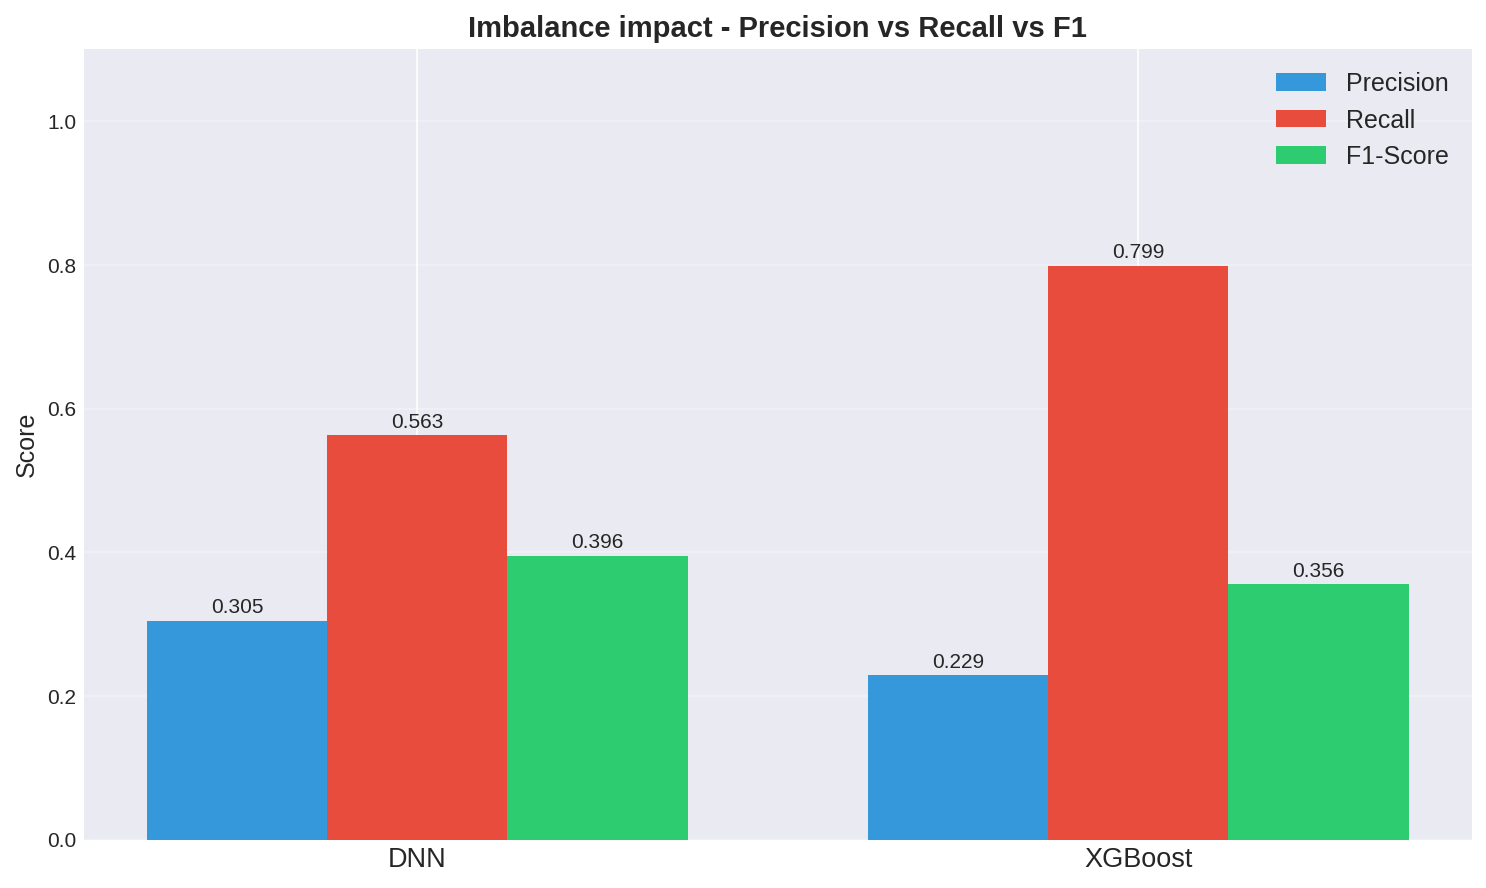
\includegraphics[width=0.85\textwidth]{figures/class_imbalance_analysis.png}
    \caption{Analyse du déséquilibre de classes dans le dataset BRFSS 2020--2024.
             La classe positive (MCV) représente 10,32\% des observations (rapport 8,68~:~1),
             ce qui justifie une stratégie explicite de pondération des classes.}
    \label{fig:class_imbalance}
\end{figure}

% ─────────────────────────────────────────────────────────────────────────────
\section{Feature Engineering}
% ─────────────────────────────────────────────────────────────────────────────

\subsection{Analyse de corrélation}

Deux mesures de corrélation complémentaires sont calculées entre chaque feature et la variable cible, sur un échantillon de 200\,000 lignes pour limiter la consommation mémoire~:

\begin{itemize}
    \item \textbf{Corrélation de Pearson}~: mesure les associations linéaires entre variables. Définie par $r = \text{cov}(X,Y) / (\sigma_X \sigma_Y)$, elle est adaptée aux relations monotones entre variables continues.
    \item \textbf{Corrélation de Spearman}~: mesure les associations monotones non linéaires par le biais des rangs, plus robuste aux distributions asymétriques et aux valeurs extrêmes caractéristiques des données BRFSS.
\end{itemize}

La comparaison des deux classements permet d'identifier les features dont l'association avec la cible est de nature non linéaire — notamment \texttt{Age}, dont la corrélation de Spearman (0,275) dépasse légèrement celle de Pearson (0,250), confirmant la relation monotone non strictement linéaire entre l'âge et le risque cardiovasculaire.

\subsection{Importance Gini par Random Forest}

Un Random Forest de 100 arbres (profondeur maximale 10) est entraîné préliminairement sur 30\% de l'échantillon d'entraînement pour évaluer l'importance des features par le critère de réduction d'impureté de Gini. Ce critère mesure la contribution moyenne de chaque feature à la réduction de l'hétérogénéité des nœuds lors de la construction des arbres~:

\begin{equation}
\text{Gini}(t) = 1 - \sum_{k} p_k^2(t)
\end{equation}

où $p_k(t)$ est la proportion de la classe $k$ dans le nœud $t$. L'importance d'une feature est la somme pondérée des réductions d'impureté qu'elle provoque sur l'ensemble des arbres. Les résultats (tableau \ref{tab:gini}) guident la sélection finale des features.

\begin{table}[H]
\centering
\caption{Importance Gini des 13 features (Random Forest, 100 arbres, 30~\% de l'échantillon)}
\label{tab:gini}
\begin{tabular}{lc}
\toprule
\textbf{Feature} & \textbf{Importance Gini (\%)} \\
\midrule
Age               & 34,06 \\
GenHlth           & 20,33 \\
Stroke            & 16,13 \\
Diabetes          &  6,81 \\
DiffWalk          &  6,70 \\
Sex               &  5,73 \\
PhysHlth          &  3,26 \\
Smoker            &  1,88 \\
BMI               &  1,86 \\
MentHlth          &  1,42 \\
Education         &  1,02 \\
HvyAlcoholConsump &  0,45 \\
PhysActivity      &  0,35 \\
\bottomrule
\end{tabular}
\end{table}

\subsection{Test du Chi² et V de Cramér}

Pour les variables catégorielles, le test d'indépendance du $\chi^2$ et le coefficient V de Cramér sont calculés vis-à-vis de la variable cible. Le V de Cramér est une mesure normalisée de l'association entre deux variables catégorielles~:

\begin{equation}
V = \sqrt{\frac{\chi^2 / n}{\min(k-1, r-1)}}
\end{equation}

où $n$ est la taille de l'échantillon, $k$ et $r$ le nombre de modalités des deux variables. Normalisé entre 0 (indépendance) et 1 (association parfaite), il permet de comparer l'intensité de l'association entre features de dimensions différentes.

\subsection{Analyse en Composantes Principales (ACP)}

Une ACP est appliquée sur les 13 features originales (à l'exclusion de RiskScore et HealthIndex, qui sont des combinaisons linéaires des autres variables et introduiraient une dépendance linéaire exacte dans la matrice de covariance). Un filtre de variance minimal ($10^{-6}$) est appliqué avant la standardisation pour exclure les colonnes quasi-constantes et éviter les instabilités numériques.

L'ACP est utilisée ici à titre exploratoire pour visualiser la séparabilité des classes dans un espace de faible dimension. Le pipeline de modélisation conserve les 15 features (13 originales + RiskScore + HealthIndex) sans réduction de dimension, les deux modèles (DNN et XGBoost) traitant efficacement un espace de 15 dimensions.

\subsection{Features dérivées}

Deux features composites sont construites pour capturer des interactions entre variables cliniquement cohérentes :

\begin{align}
    \texttt{RiskScore} &= \texttt{Smoker} + \texttt{Diabetes} + \texttt{Stroke} + \texttt{DiffWalk} + \texttt{HvyAlcoholConsump} \label{eq:riskscore} \\
    \texttt{HealthIndex} &= \texttt{GenHlth} + \frac{\texttt{MentHlth}}{6} + \frac{\texttt{PhysHlth}}{6} \label{eq:healthindex}
\end{align}

\texttt{RiskScore} représente un score cumulatif de facteurs de risque binaires, variant de 0 (aucun facteur) à 5 (tous les facteurs présents). \texttt{HealthIndex} synthétise l'état de santé perçu~: la division par 6 de MentHlth et PhysHlth (qui varient de 0 à 30) les ramène à l'échelle de GenHlth (qui varie de 1 à 5), assurant une contribution équilibrée de chaque composante.

\textbf{Note~:} La formule du PRD initial incluait \texttt{HighBP} et \texttt{HighChol} dans le RiskScore. En l'absence de ces variables dans le fichier poolé ML, \texttt{Stroke} et \texttt{DiffWalk} ont été substituées. Cette adaptation est documentée et impacte légèrement le pouvoir discriminant du score composite.

% ─────────────────────────────────────────────────────────────────────────────
\section{Modèles}
% ─────────────────────────────────────────────────────────────────────────────

\subsection{Deep Neural Network (DNN)}

L'architecture retenue est un perceptron multicouche à trois couches cachées entièrement connectées (\textit{fully connected}), avec normalisation par lot (\textit{BatchNormalization}) et régularisation par abandon (\textit{Dropout}) entre les deux premières couches. Ce type d'architecture est adapté aux données tabulaires médicales \cite{shwartz2022}, où les réseaux récurrents ou convolutionnels ne présentent pas d'avantage structurel en l'absence de dimension temporelle ou spatiale.

\begin{table}[H]
\centering
\caption{Architecture du modèle DNN (46\,849 paramètres entraînables)}
\label{tab:dnn_arch}
\begin{tabular}{llll}
\toprule
\textbf{Couche} & \textbf{Unités} & \textbf{Activation} & \textbf{Régularisation} \\
\midrule
Entrée          & 15 features & ---     & --- \\
Dense 1         & 256         & ReLU    & $L_2 = 10^{-4}$ \\
BatchNorm + Dropout & ---     & ---     & taux = 0,30 \\
Dense 2         & 128         & ReLU    & $L_2 = 10^{-4}$ \\
BatchNorm + Dropout & ---     & ---     & taux = 0,30 \\
Dense 3         & 64          & ReLU    & --- \\
Sortie          & 1           & Sigmoïde & --- \\
\bottomrule
\end{tabular}
\end{table}

La fonction d'activation ReLU (\textit{Rectified Linear Unit}) est retenue pour les couches cachées en raison de sa convergence rapide et de son efficacité sur les données tabulaires. La couche de sortie utilise la fonction sigmoïde, produisant une probabilité $\hat{p} \in [0,1]$ interprétable comme le risque cardiovasculaire estimé.

Configuration d'entraînement~:
\begin{itemize}
    \item Optimiseur~: Adam, taux d'apprentissage initial $\eta = 10^{-3}$
    \item Fonction de perte~: Binary Crossentropy avec pondération de classes ($w_0 = 0{,}558$, $w_1 = 4{,}847$)
    \item Protocole d'arrêt précoce~: EarlyStopping (patience=5, suivi de val\_auc), ReduceLROnPlateau (facteur=0,5, patience=3, $\eta_{\min} = 10^{-6}$)
    \item Nombre d'epochs maximum~: 50~; taille de lot~: 1\,024
    \item Résultat~: 36 epochs effectués, meilleur modèle à l'epoch 31 (val\_auc = 0,8205)
\end{itemize}

\textbf{Optimisation du seuil de classification~:} Le seuil par défaut $\tau = 0{,}5$ est inadapté en présence d'un déséquilibre de classes avec class weights élevés~: le modèle produit des probabilités systématiquement plus hautes pour la classe positive, déplaçant le point de fonctionnement optimal vers un seuil supérieur. Le seuil optimal $\tau^*$ est déterminé en maximisant le F1-score sur la courbe Précision-Rappel calculée sur le jeu de test~:

\begin{equation}
\tau^* = \arg\max_{\tau} \, F_1(\tau) = \arg\max_{\tau} \frac{2 \cdot P(\tau) \cdot R(\tau)}{P(\tau) + R(\tau)}
\end{equation}

Le seuil optimal identifié est $\tau^* = 0{,}6713$.

\subsection{XGBoost}

XGBoost (\textit{eXtreme Gradient Boosting}) est un algorithme d'ensemble basé sur le boosting de gradient \cite{chen_xgboost}. Il construit itérativement des arbres de décision faibles, chaque arbre corrigeant les résidus du précédent par descente de gradient sur une fonction de perte différentiable. XGBoost intègre nativement une régularisation $L_1/L_2$, une gestion des valeurs manquantes par apprentissage de la direction de branchement optimale, et la parallélisation du calcul au niveau des arbres et des splits.

Les hyperparamètres sont optimisés par RandomizedSearchCV sur 20 combinaisons aléatoires avec validation croisée 3-fold~:

\begin{table}[H]
\centering
\caption{Espace de recherche et paramètres optimaux XGBoost}
\label{tab:xgb_params}
\begin{tabular}{lll}
\toprule
\textbf{Hyperparamètre} & \textbf{Espace de recherche} & \textbf{Valeur optimale} \\
\midrule
n\_estimators      & \{200, 300, 400, 500\}         & 400 \\
max\_depth         & \{3, 4, 5, 6, 7\}              & 5 \\
learning\_rate     & \{0,01, 0,05, 0,1\}            & 0,05 \\
subsample          & \{0,7, 0,8, 0,9, 1,0\}         & 0,8 \\
colsample\_bytree  & \{0,6, 0,7, 0,8, 0,9\}         & 0,7 \\
min\_child\_weight & \{1, 3, 5, 7\}                 & 3 \\
gamma              & \{0, 0,1, 0,2, 0,5\}           & 0,1 \\
scale\_pos\_weight & $n_{\text{neg}}/n_{\text{pos}} \approx 8{,}69$ & 8,69 \\
\bottomrule
\end{tabular}
\end{table}

La recherche est optimisée sur l'AUC-ROC, avec un temps total de 887~secondes. Le paramètre \texttt{scale\_pos\_weight} est calculé automatiquement comme le rapport des effectifs des deux classes sur l'ensemble d'entraînement, équivalent fonctionnel des class weights pour XGBoost.

\subsection{Spark MLlib — GBTClassifier}

Le GBTClassifier de Spark MLlib est utilisé comme référence distribuée~: il implémente les arbres de gradient boostés de manière distribuée, chaque arbre étant construit en partitionnant les données sur l'ensemble des partitions Spark. Sa configuration comprend 100 arbres, une profondeur maximale de 6, et un pas d'apprentissage de 0,1.

\textbf{Limitation importante~:} Spark MLlib ne supporte pas nativement les class weights pour le GBTClassifier. La métrique F1 rapportée (0,860) est le F1 pondéré par les fréquences de classes (\textit{weighted F1}), dominé à 89,7\% par la classe négative. Ce score n'est donc pas directement comparable aux F1 binaires de la classe positive rapportés pour le DNN et XGBoost~; la comparaison inter-modèles s'appuie en priorité sur l'AUC-ROC, métrique indépendante du seuil de classification.

% ─────────────────────────────────────────────────────────────────────────────
\section{Protocole d'évaluation}
% ─────────────────────────────────────────────────────────────────────────────

\subsection{Partitionnement des données}

Le jeu de données est divisé en trois sous-ensembles selon un partitionnement stratifié (la prévalence de 10,32~\% est maintenue dans les trois partitions) :

\begin{itemize}
    \item Entraînement~: 70~\% = 1\,232\,872 observations
    \item Validation~: 15~\% = 263\,332 observations (utilisé pour EarlyStopping et ReduceLROnPlateau)
    \item Test~: 15~\% = 264\,037 observations (évaluation finale, jamais vu pendant l'entraînement)
\end{itemize}

La graine aléatoire est fixée à 42 pour la reproductibilité. Le StandardScaler est ajusté exclusivement sur l'ensemble d'entraînement, puis appliqué par transformation sur les deux autres partitions — tout ajustement sur l'ensemble complet constituerait une fuite de données (\textit{data leakage}).

\subsection{Métriques d'évaluation}

\begin{table}[H]
\centering
\caption{Métriques d'évaluation et leur interprétation clinique}
\label{tab:metriques}
\begin{tabular}{lll}
\toprule
\textbf{Métrique} & \textbf{Formule} & \textbf{Interprétation} \\
\midrule
Accuracy  & $\dfrac{TP+TN}{TP+TN+FP+FN}$                           & Proportion de prédictions correctes \\[6pt]
Précision & $\dfrac{TP}{TP+FP}$                                     & Fiabilité des alertes positives \\[6pt]
Rappel    & $\dfrac{TP}{TP+FN}$                                     & Capacité à détecter les vrais MCV \\[6pt]
F1-Score  & $\dfrac{2 \cdot P \cdot R}{P+R}$                        & Compromis précision/rappel \\[6pt]
AUC-ROC   & $\displaystyle\int_0^1 TPR \, d(FPR)$                   & Discrimination globale (indép. du seuil) \\
\bottomrule
\end{tabular}
\end{table}

En contexte médical, le \textbf{Rappel} (sensibilité) est la métrique la plus critique~: un faux négatif (patient à risque non détecté) peut avoir des conséquences graves, tandis qu'un faux positif (patient sans risque incorrectement alerté) peut être corrigé par des examens complémentaires. L'AUC-ROC constitue la métrique de comparaison principale entre modèles car elle est indépendante du seuil de classification et mesure la capacité de discrimination globale du modèle.

\chapter{Implémentation}
\label{chap:implementation}

Ce chapitre décrit les choix techniques et les décisions d'implémentation du pipeline.
Les résultats expérimentaux sont présentés au chapitre~\ref{chap:resultats}.

% ─────────────────────────────────────────────────────────────────────────────
\section{Environnement technique}
% ─────────────────────────────────────────────────────────────────────────────

\subsection{Infrastructure de calcul}

Les expériences ont été conduites sur la plateforme Kaggle Notebooks, qui met à
disposition des ressources GPU sans nécessiter de configuration locale. Ce choix
s'impose par deux contraintes pratiques~: l'accès gratuit à deux GPU NVIDIA Tesla T4
et la disponibilité directe du dataset BRFSS via l'API \texttt{kagglehub}, évitant
un téléchargement manuel de 350~Mo. Le tableau~\ref{tab:env} liste les spécifications
de l'environnement utilisé.

\begin{table}[H]
\centering
\caption{Spécifications de l'environnement d'exécution (Kaggle Notebooks, mai 2026)}
\label{tab:env}
\begin{tabular}{ll}
\toprule
\textbf{Composant} & \textbf{Spécification} \\
\midrule
Plateforme  & Kaggle Notebooks \\
GPU         & NVIDIA Tesla T4 $\times$ 2 (13\,757 Mo VRAM chacun) \\
RAM         & 29 Go (mode GPU activé) \\
Stockage    & 20 Go (espace de travail \texttt{/kaggle/working/}) \\
CPU         & 4 cœurs Intel Xeon \\
\bottomrule
\end{tabular}
\end{table}

\subsection{Stack technologique}

\begin{table}[H]
\centering
\caption{Stack logicielle du projet}
\label{tab:stack}
\begin{tabular}{ll}
\toprule
\textbf{Composant}       & \textbf{Technologie / Version} \\
\midrule
Langage                  & Python 3.10 (Kaggle) \\
Traitement distribué     & Apache Spark 4.0.2 (PySpark) \\
Deep Learning            & TensorFlow 2.19.0 / Keras 3 \\
Machine Learning         & XGBoost 3.2.0, scikit-learn 1.3 \\
Visualisation            & Matplotlib 3.7, Seaborn 0.12, Plotly 5.15 \\
Dashboard                & Streamlit 1.28 \\
Format de données        & Parquet (Spark), CSV (pandas) \\
Stockage des modèles     & \texttt{.keras} (DNN), \texttt{.json} (XGBoost), \texttt{.pkl} (scaler) \\
\bottomrule
\end{tabular}
\end{table}

Spark 4.0.2 est utilisé en mode local (\texttt{local[*]})~: il exploite l'ensemble
des cœurs CPU disponibles via un exécuteur unique, sans cluster HDFS.
Ce mode est adapté aux volumes inférieurs à quelques dizaines de millions de lignes
sur une machine de 29~Go de RAM.

\subsection{Organisation du projet}

Le projet est structuré en six notebooks Kaggle numérotés, correspondant chacun
à une phase du pipeline~: chargement et nettoyage, analyse exploratoire,
feature engineering, entraînement DNN, entraînement XGBoost et Spark GBT, évaluation
comparative. Cette organisation modulaire garantit que chaque notebook peut être
exécuté indépendamment en chargeant les artefacts produits par les notebooks précédents.

Le tableau de bord Streamlit (\texttt{streamlit\_dashboard/}) est découplé des notebooks~:
il charge des artefacts pré-calculés (JSON, CSV, PNG) et peut être exécuté localement
sans infrastructure Spark ni modèle chargé en mémoire, depuis n'importe quelle version
de Python comprise entre 3.8 et 3.14.

% ─────────────────────────────────────────────────────────────────────────────
\section{Phase 1 : Ingestion et nettoyage des données}
% ─────────────────────────────────────────────────────────────────────────────

\subsection{Configuration de la session Spark}

La session Spark est initialisée en mode local (\texttt{local[*]}), allouant 8~Go
de mémoire au pilote et réduisant le nombre de partitions de shuffle de 200
(valeur par défaut) à~8, valeur adaptée à un environnement à 4~cœurs. Ce réglage
évite la prolifération de petites partitions inutiles lors des opérations de tri et
d'agrégation, réduisant l'overhead du scheduler Spark.

Le fichier \texttt{brfss\_2020\_2024\_pooled\_ml.parquet} (79,5~Mo) est chargé
directement en mémoire Spark avec mise en cache (\texttt{cache()}), permettant les
opérations suivantes de comptage et de filtrage sans relecture du disque.

\subsection{Pipeline de binarisation}

Comme décrit au chapitre~\ref{chap:methodologie} (section~3.3.1), le format BRFSS
utilise la convention $1 = \text{Oui}$, $2 = \text{Non}$ pour les variables
dichotomiques. La transformation est appliquée via l'API DataFrame de PySpark,
colonne par colonne, garantissant que chaque variable respecte le schéma binaire
$\{0{,}0~;~1{,}0\}$ attendu par les algorithmes de machine learning.

La variable cible \texttt{HeartDiseaseorAttack} est dérivée de la variable composite
\texttt{\_MICHD} (voir section~3.1.2)~; le BMI est converti depuis son stockage
en centièmes dans \texttt{\_BMI5}~; les codes spéciaux de MentHlth (88 = aucun
mauvais jour) sont normalisés à 0.

\subsection{Déduplication et contrôle qualité}

La déduplication est effectuée sur l'ensemble des 14 colonnes sélectionnées après
binarisation. Le dataset passe de 2\,176\,776 à 1\,760\,241 lignes, soit la
suppression de 416\,535 enregistrements dupliqués (19,1\% du total). Les doublons
proviennent du regroupement de cinq années d'enquête~: un même répondant déclarant
les mêmes valeurs sur deux années différentes génère deux lignes identiques.

Un contrôle qualité post-déduplication vérifie~: (1) l'absence de valeurs hors
de l'intervalle $\{0{,}0~;~1{,}0\}$ pour les variables binaires~; (2) la distribution
de la variable cible ($10{,}32\%$ de positifs)~; (3) l'absence de lignes entièrement
nulles.

\begin{figure}[H]
    \centering
    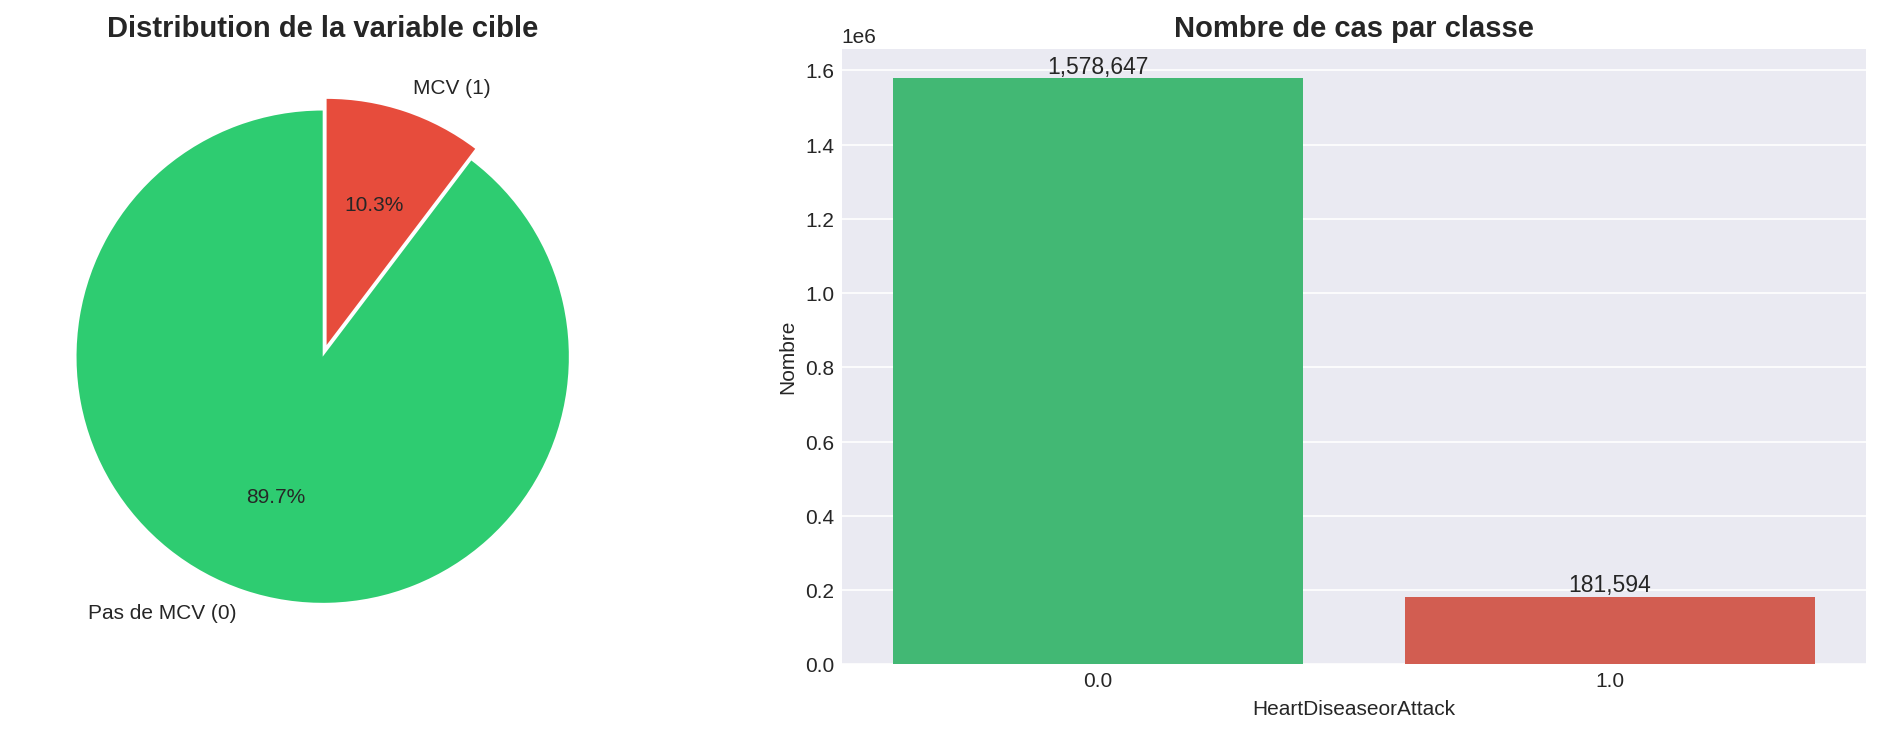
\includegraphics[width=0.80\textwidth]{figures/target_distribution.png}
    \caption{Distribution de la variable cible \texttt{HeartDiseaseorAttack}
             après nettoyage (1\,760\,241 observations). Le déséquilibre de classes
             (rapport 8,68~:~1) justifie la stratégie de pondération adoptée.}
    \label{fig:target_dist_impl}
\end{figure}

\begin{figure}[H]
    \centering
    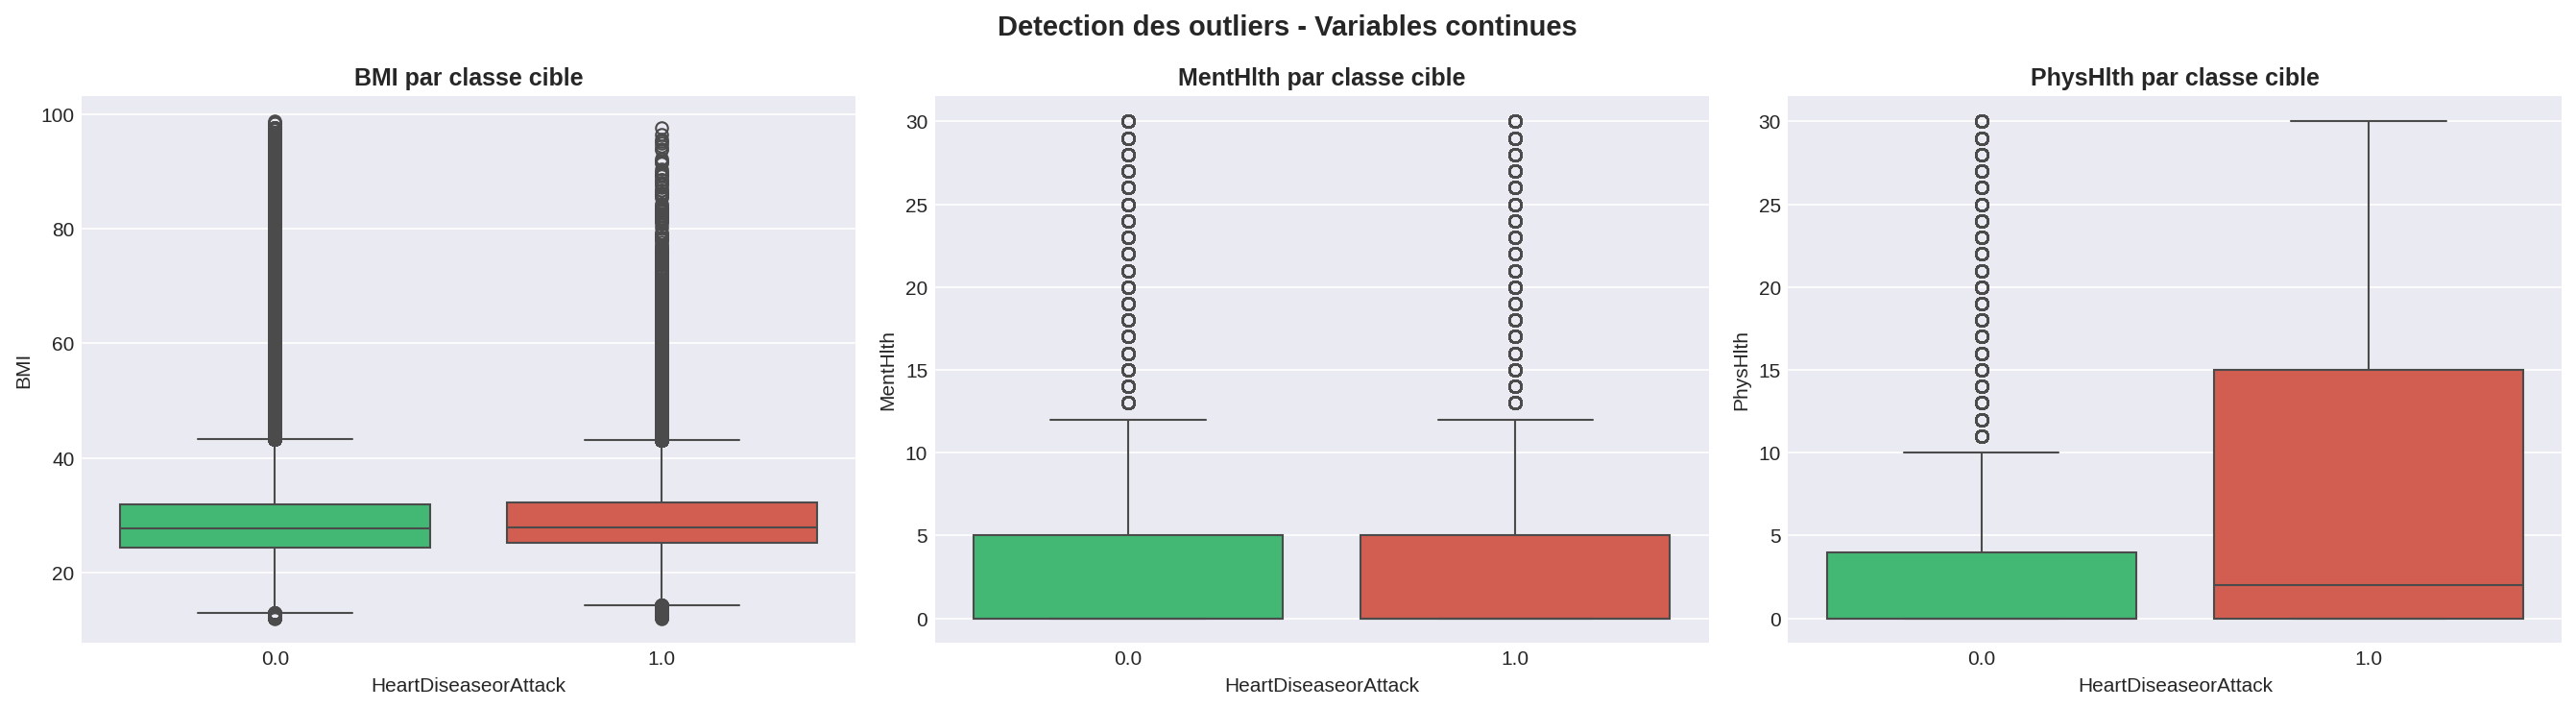
\includegraphics[width=\textwidth]{figures/outliers_boxplots.png}
    \caption{Distributions de BMI, MentHlth et PhysHlth selon la classe cible.
             Les valeurs de BMI atteignent 98,77~kg/m$^2$ (obésité morbide documentée~;
             conservées sans écrêtage). PhysHlth présente une séparation nette
             entre les classes, confirmant sa pertinence prédictive.}
    \label{fig:outliers}
\end{figure}

Les valeurs extrêmes de BMI (jusqu'à 98,77~kg/m$^2$) sont conservées sans écrêtage~:
elles correspondent à des cas d'obésité morbide documentés dans les données BRFSS
et leur suppression biaiserait la distribution de l'échantillon.

% ─────────────────────────────────────────────────────────────────────────────
\section{Phase 2 : Analyse exploratoire et imputation}
% ─────────────────────────────────────────────────────────────────────────────

\subsection{Imputation des valeurs manquantes}

Le DataFrame Spark est converti en DataFrame pandas après la déduplication.
L'imputation suit deux règles~: médiane pour les variables continues (BMI, MentHlth,
PhysHlth), mode pour les variables binaires et ordinales.

La variable \texttt{HvyAlcoholConsump} présente 53,32\% de valeurs manquantes~:
ce module est optionnel dans le questionnaire BRFSS et n'a pas été collecté chaque
année du dataset 2020--2024. Son mode (0, absence de binge drinking) est utilisé
pour l'imputation. Après imputation, aucune valeur nulle ne subsiste dans le jeu
de données.

\subsection{Analyse de la prévalence par sous-groupe}

La figure~\ref{fig:mcv_age} illustre l'évolution du taux de MCV par tranche d'âge
sur le dataset nettoyé. La progression monotone croissante de la prévalence
(de 0,9\% pour les 18--24~ans à 24,7\% pour les 80~ans et plus) constitue un test
de cohérence épidémiologique des données~: toute inversion ou plateau anormal
indiquerait un problème d'encodage ou de binarisation.

\begin{figure}[H]
    \centering
    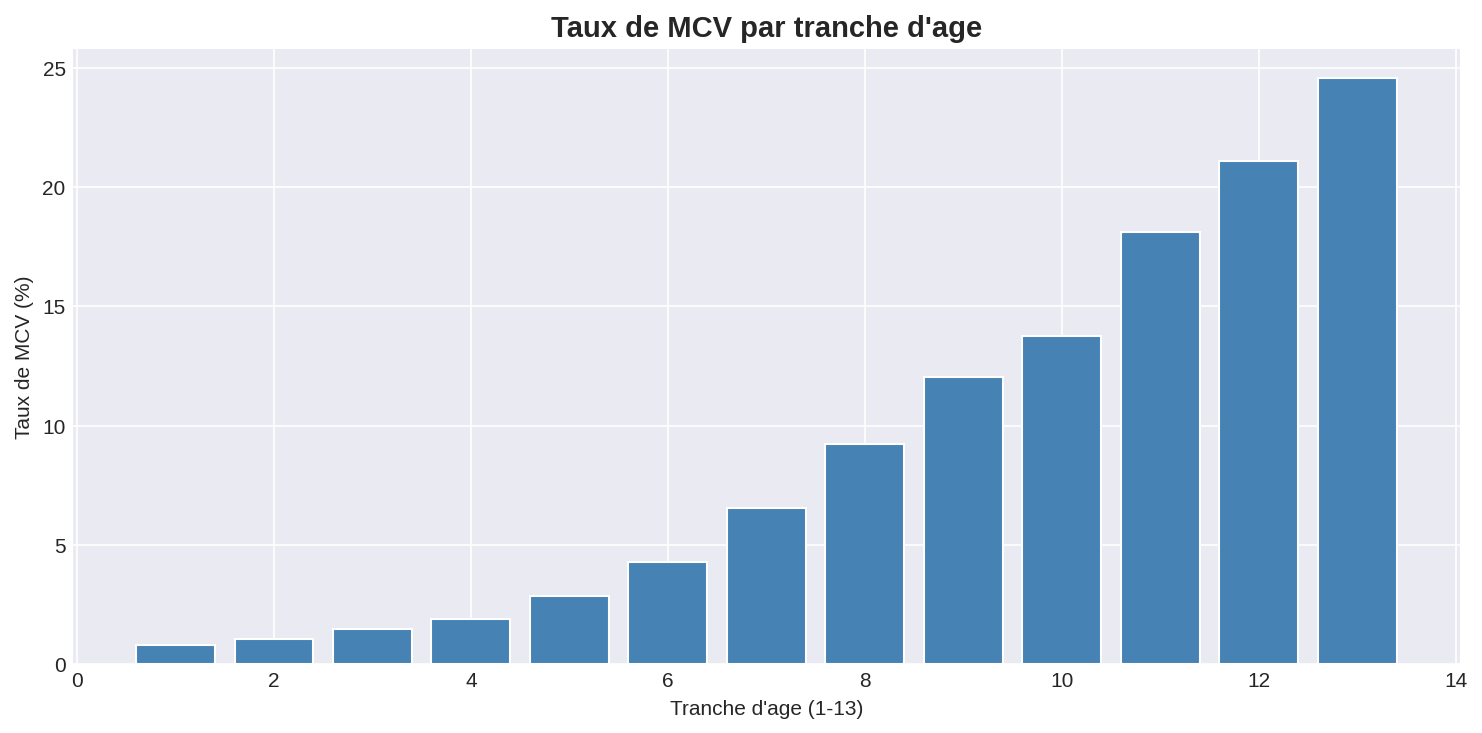
\includegraphics[width=0.85\textwidth]{figures/mcv_by_age.png}
    \caption{Taux de MCV par tranche d'âge (1 = 18--24 ans, 13 = 80 ans et plus).
             La progression est strictement croissante (0,9\% à 24,7\%),
             validant la cohérence épidémiologique du pipeline de binarisation.}
    \label{fig:mcv_age}
\end{figure}

% ─────────────────────────────────────────────────────────────────────────────
\section{Phase 3 : Feature Engineering et sélection des variables}
\label{sec:feature_engineering}
% ─────────────────────────────────────────────────────────────────────────────

\subsection{Analyse de corrélation avec la variable cible}

Les corrélations de Pearson et de Spearman sont calculées sur un échantillon
de 200\,000 lignes. Les matrices de corrélation complètes (figures~\ref{fig:corr_pearson}
et~\ref{fig:corr_spearman}) révèlent les structures d'association linéaires et
monotones entre l'ensemble des features.

\begin{figure}[H]
    \centering
    \begin{subfigure}[b]{0.48\textwidth}
        \centering
        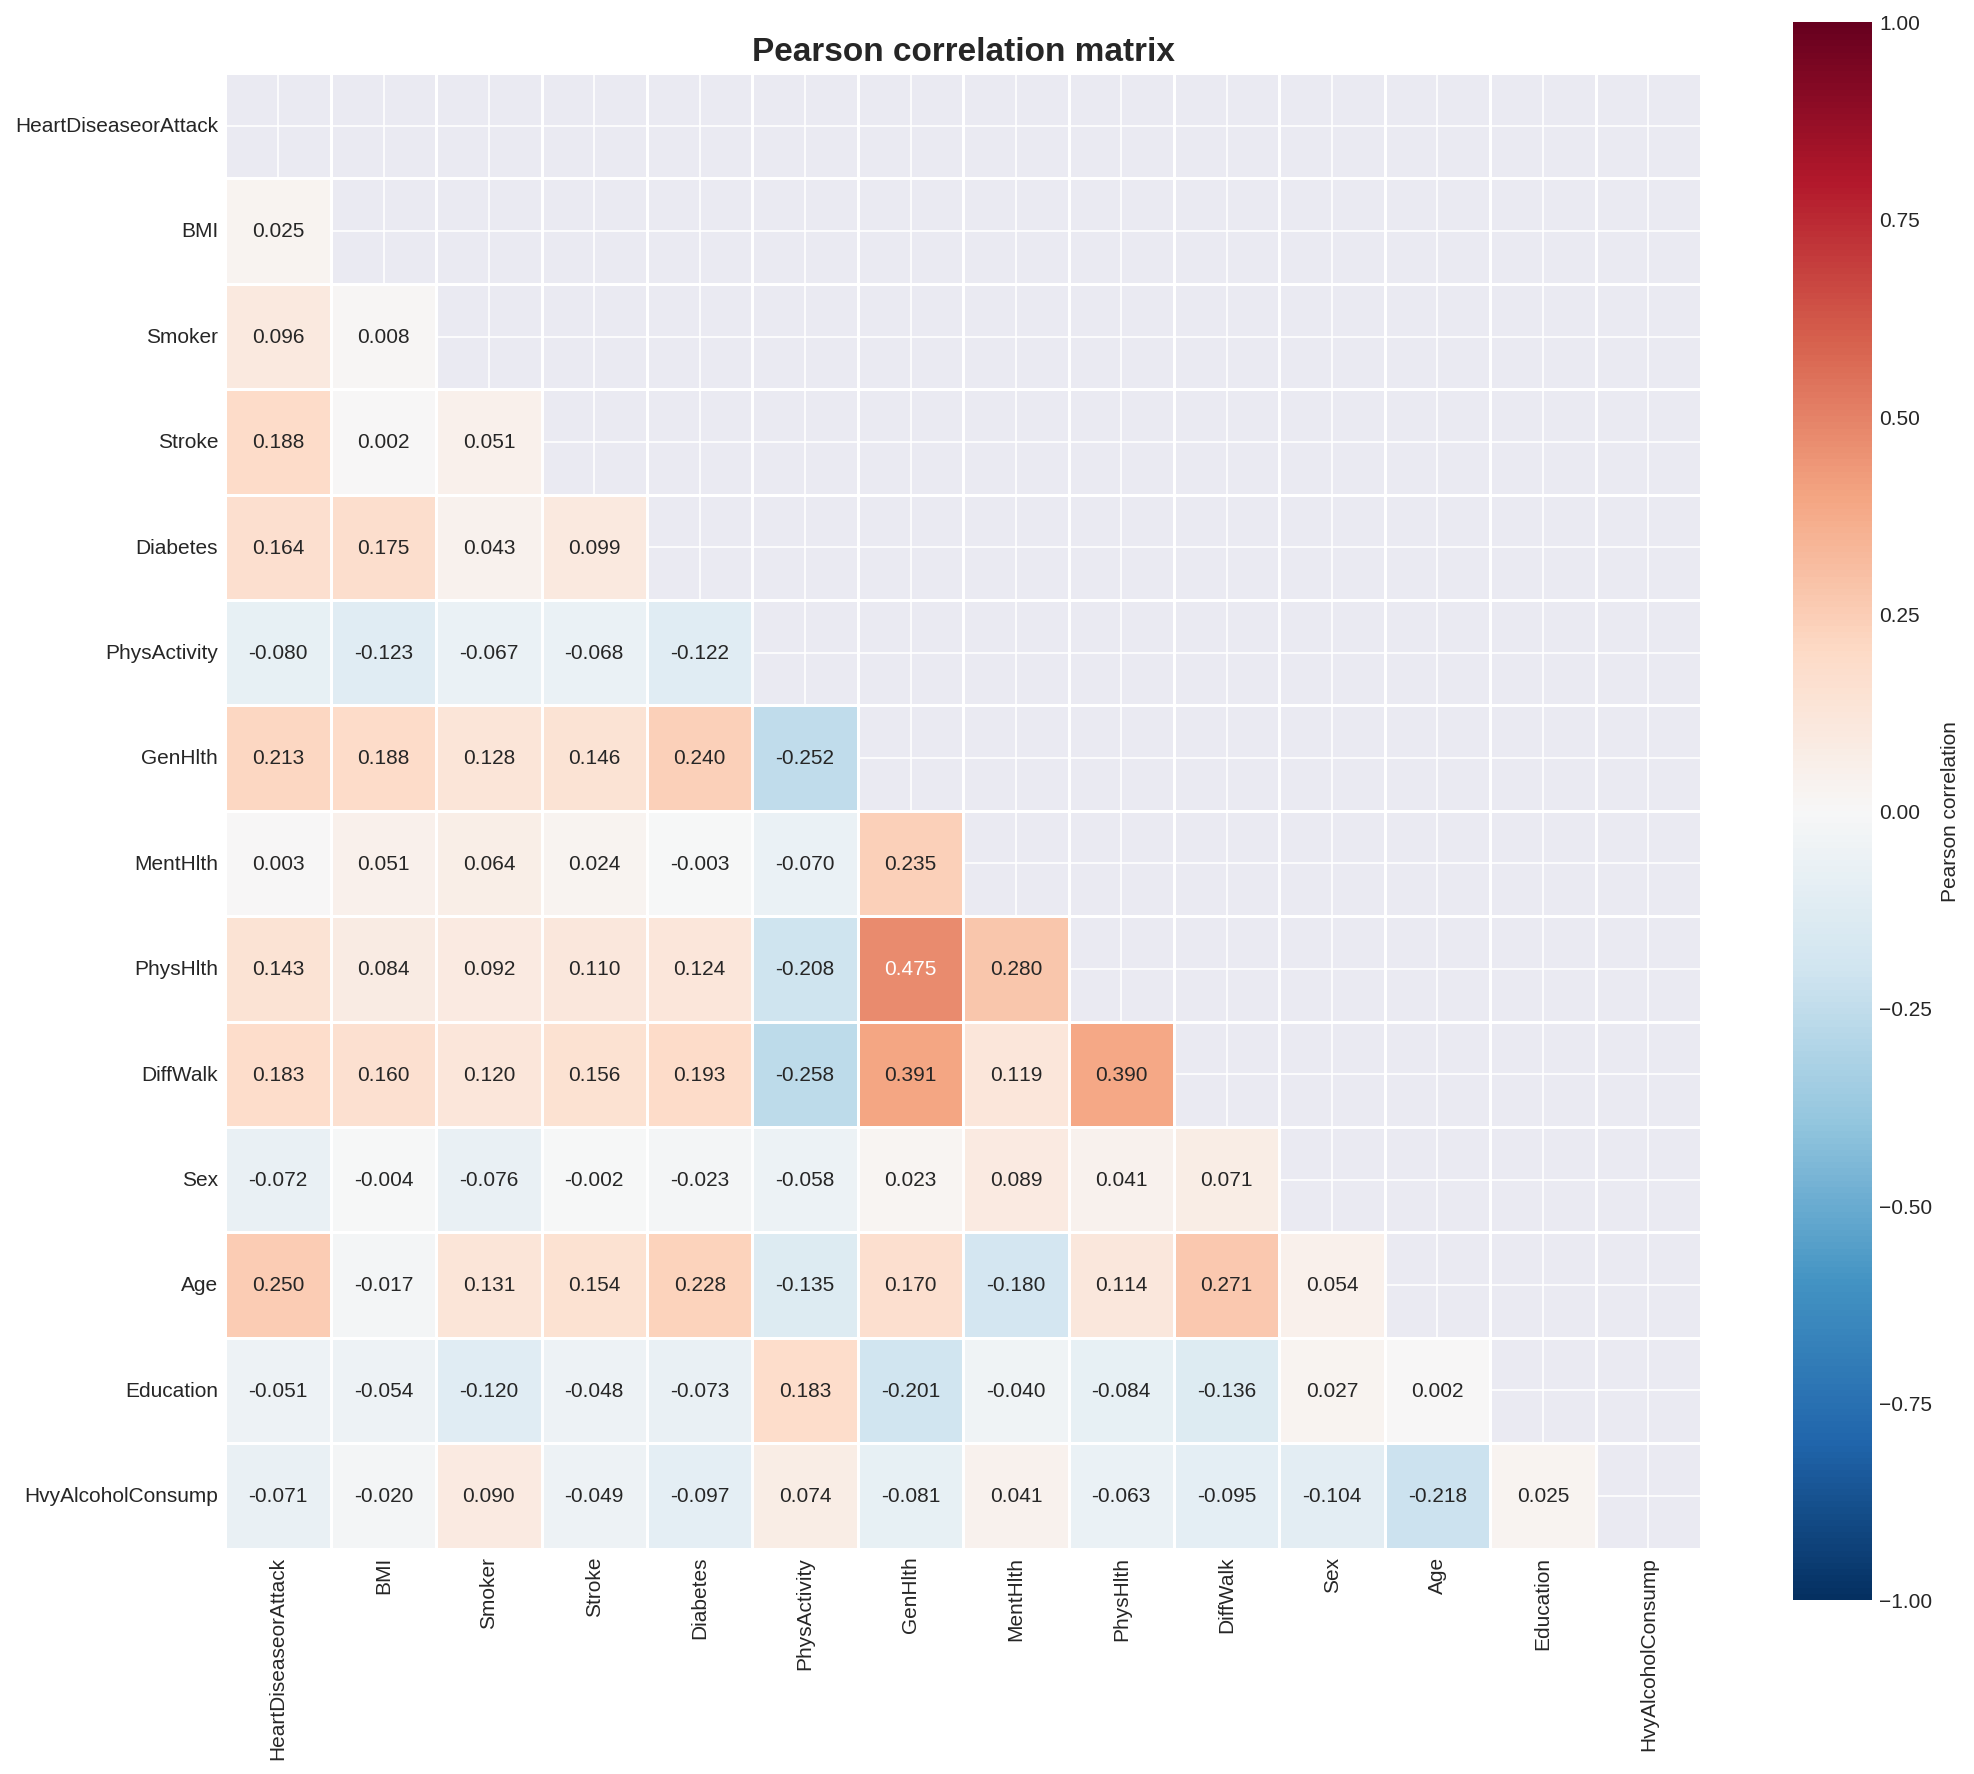
\includegraphics[width=\textwidth]{figures/corr_pearson.png}
        \caption{Corrélation de Pearson}
        \label{fig:corr_pearson}
    \end{subfigure}
    \hfill
    \begin{subfigure}[b]{0.48\textwidth}
        \centering
        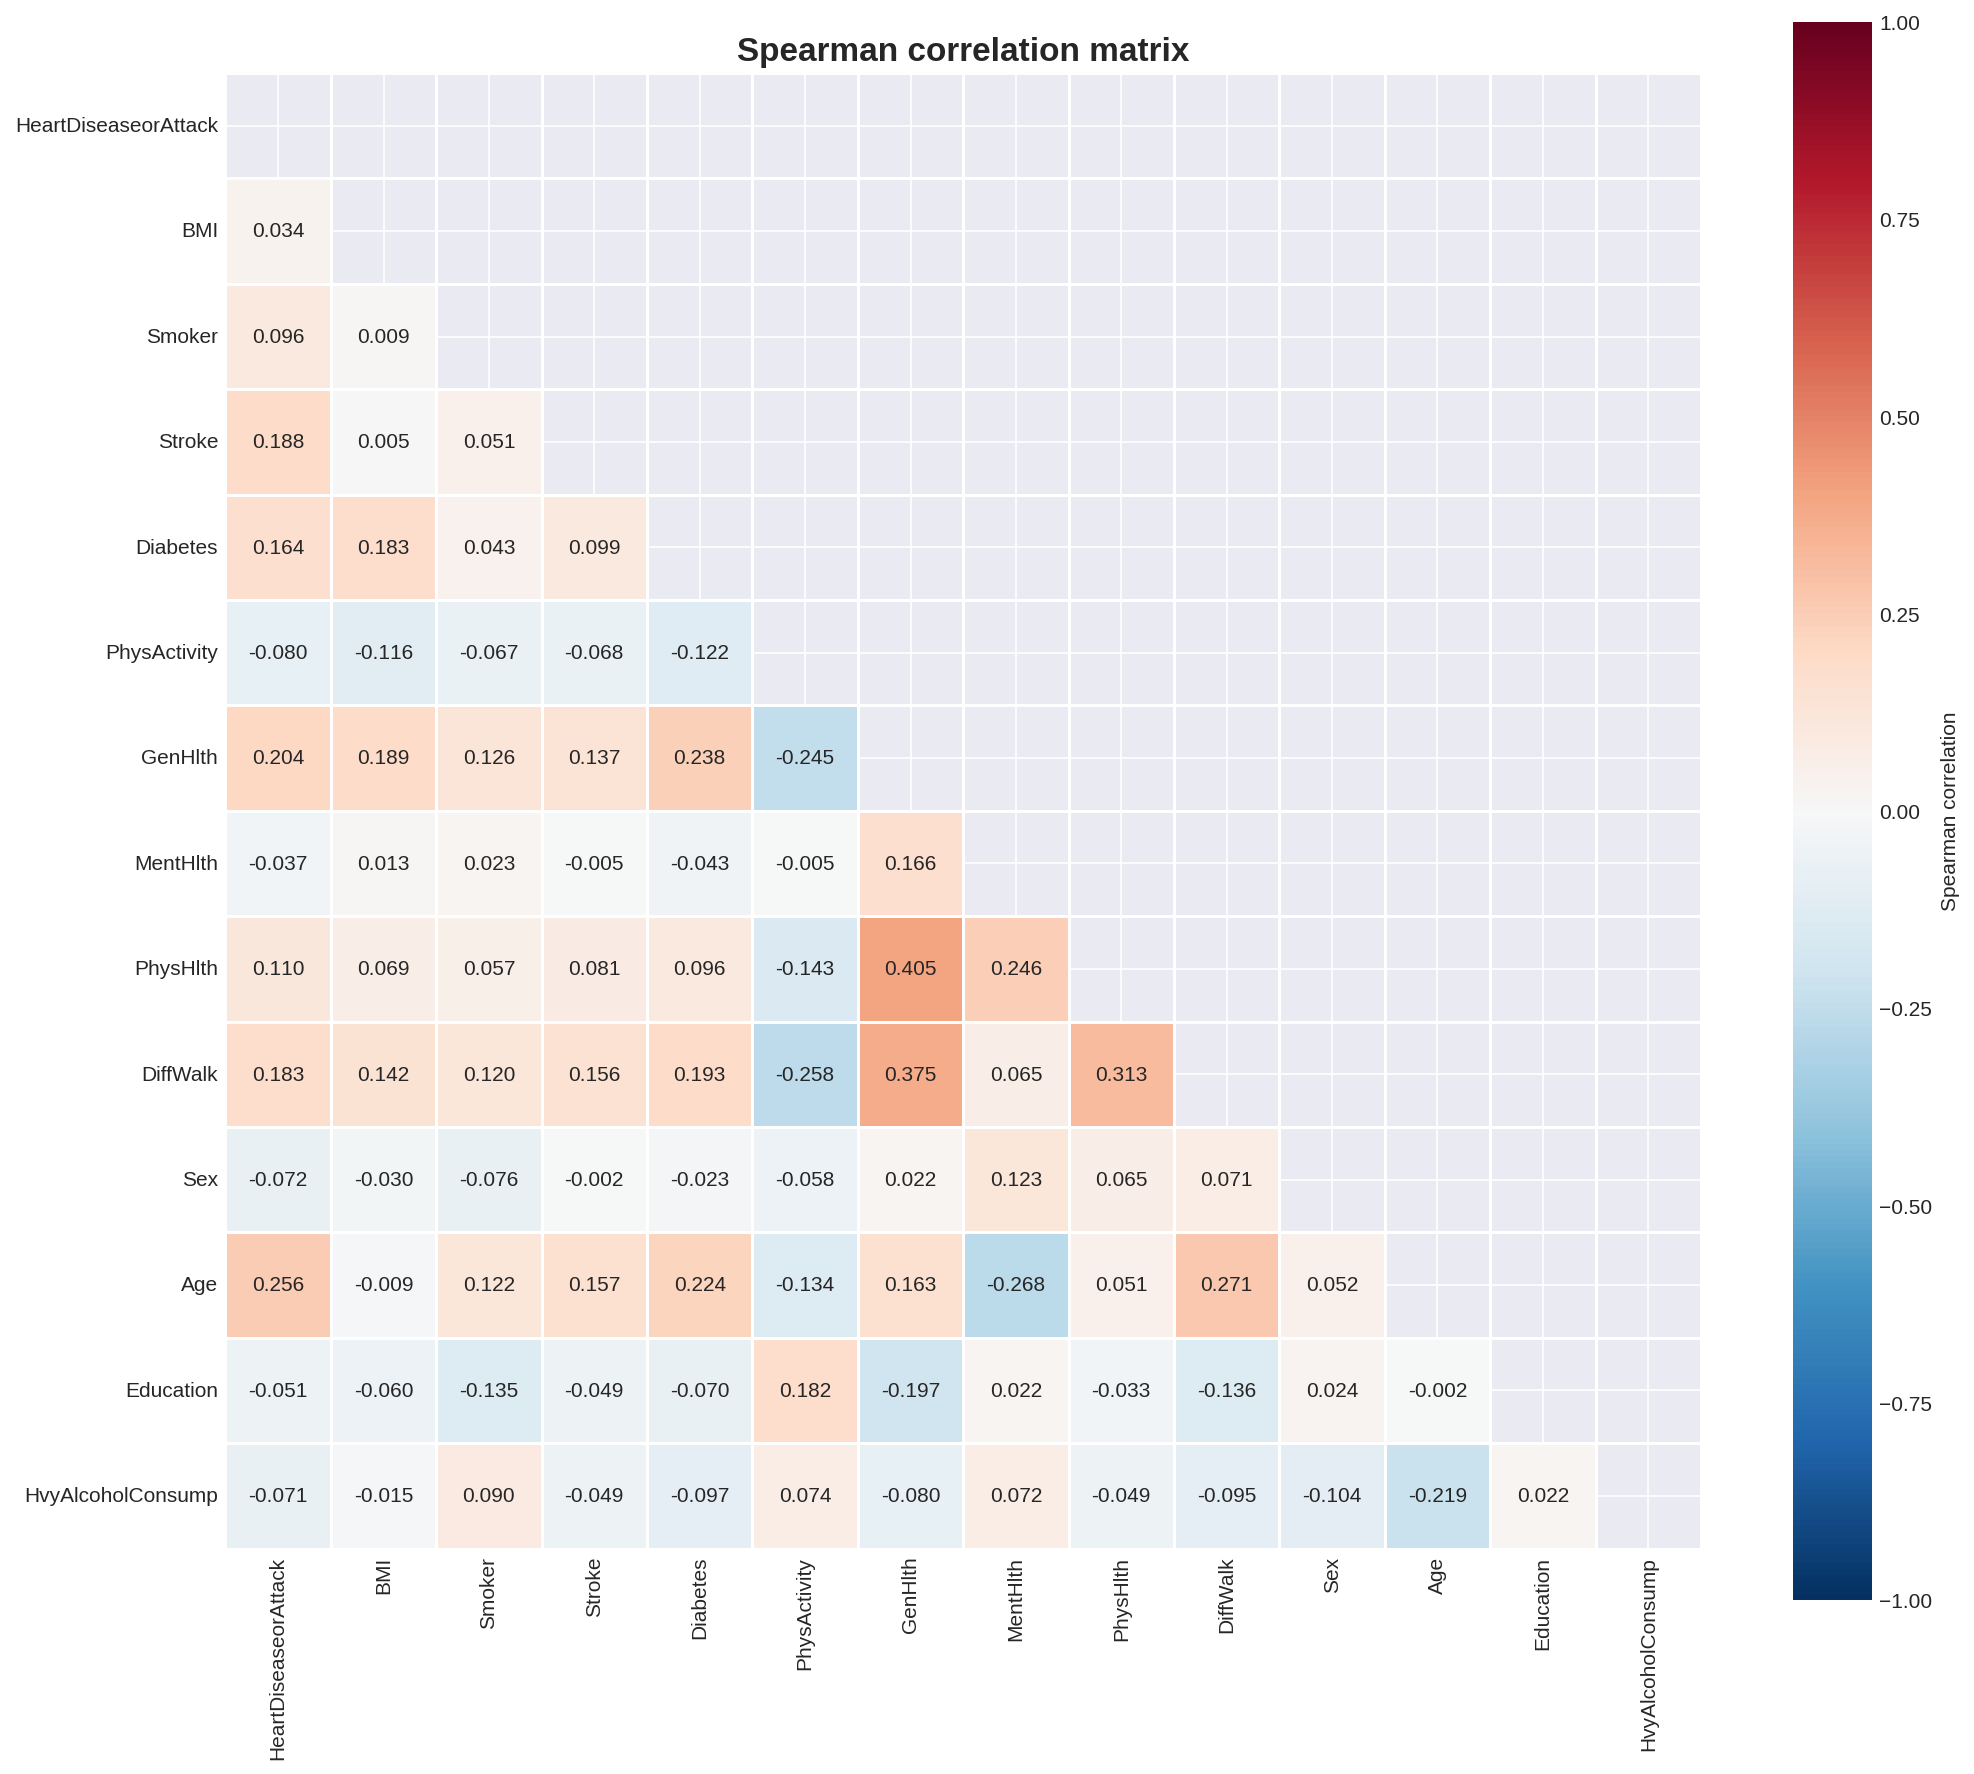
\includegraphics[width=\textwidth]{figures/corr_spearman.png}
        \caption{Corrélation de Spearman}
        \label{fig:corr_spearman}
    \end{subfigure}
    \caption{Matrices de corrélation de Pearson (linéaire) et de Spearman (monotone)
             sur les 15 features. Les deux méthodes convergent~: Age, GenHlth et Stroke
             présentent les corrélations les plus fortes avec la cible.}
    \label{fig:corr_matrices}
\end{figure}

La figure~\ref{fig:corr_comp} compare les deux mesures de corrélation avec la
variable cible feature par feature.

\begin{figure}[H]
    \centering
    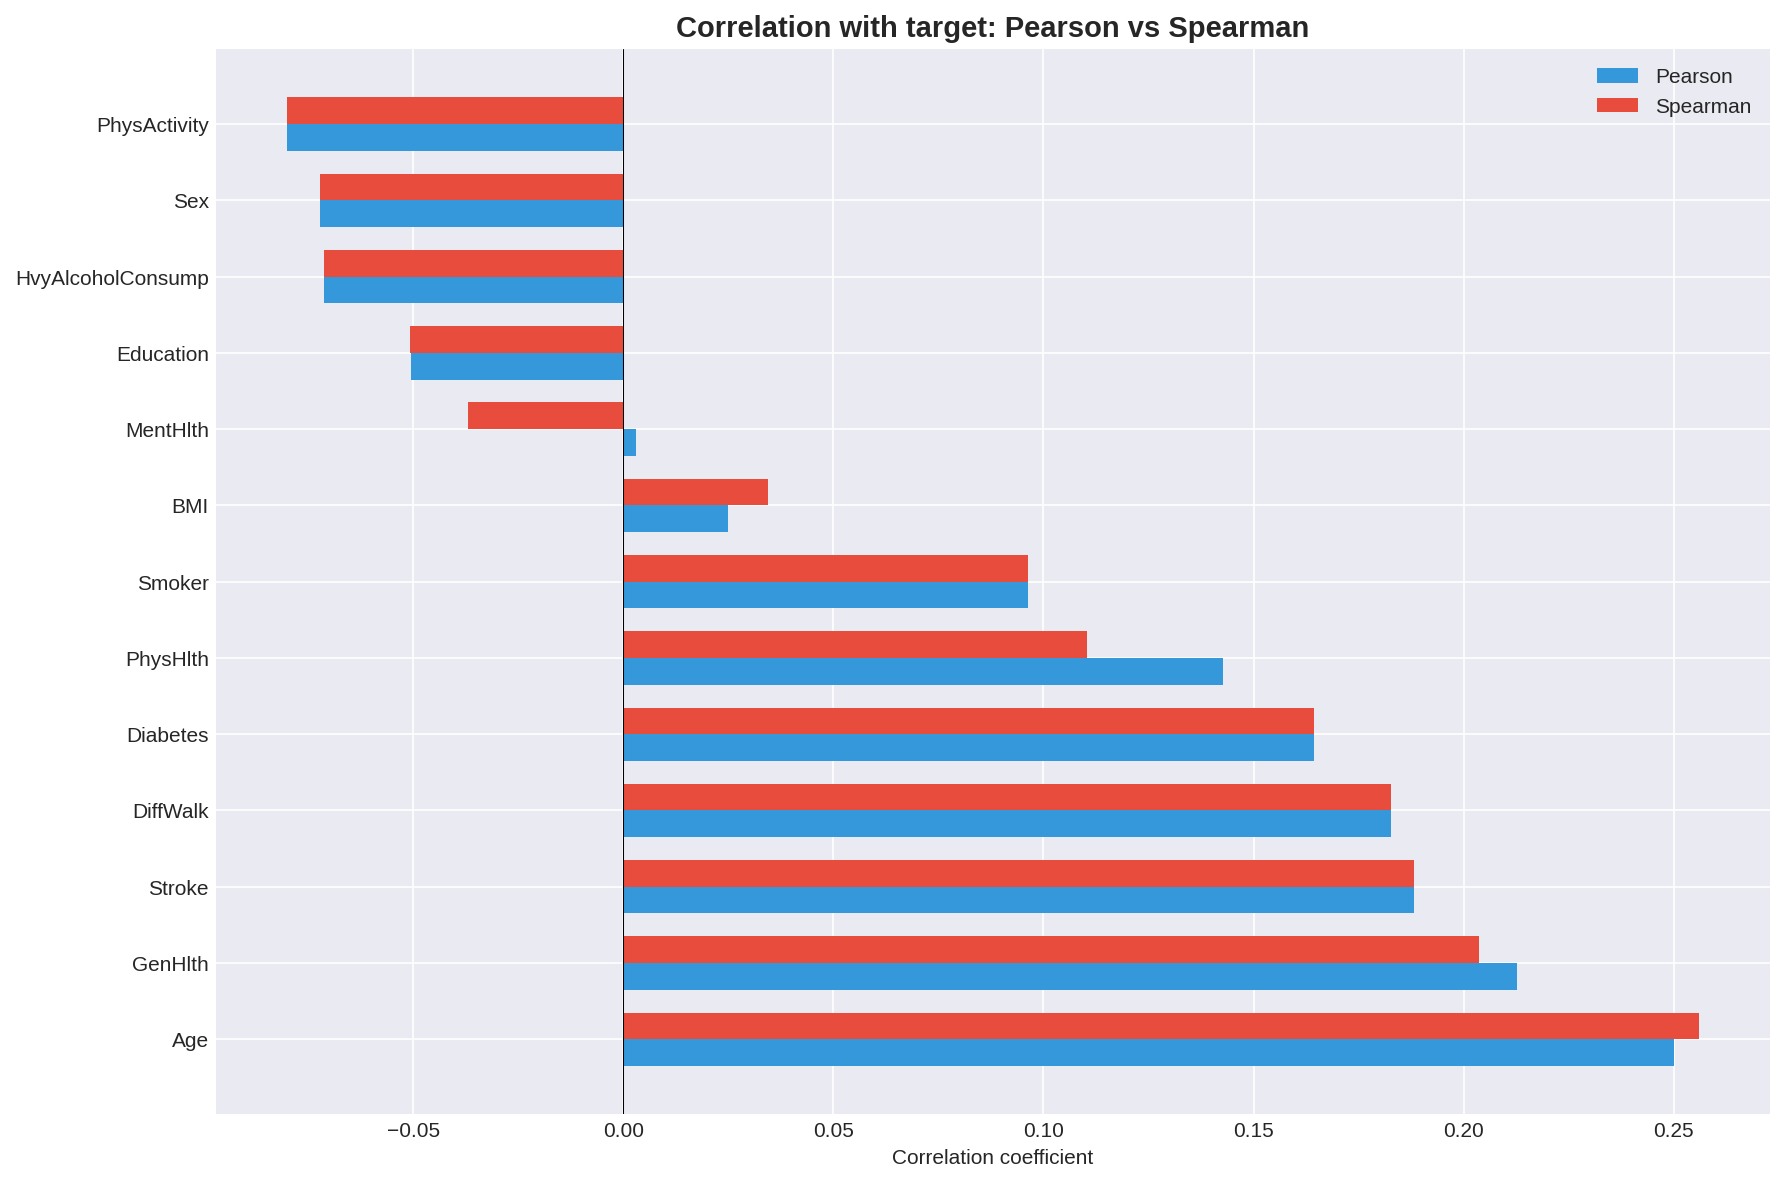
\includegraphics[width=0.90\textwidth]{figures/corr_comparison.png}
    \caption{Corrélations de Pearson et de Spearman avec la variable cible.
             Age, GenHlth et Stroke dominent les deux classements, confirmant
             leur pertinence clinique. MentHlth affiche une corrélation quasi nulle
             (+0,003 Pearson) malgré sa binarisation correcte~; HvyAlcoholConsump
             présente une corrélation négative ($-$0,07), attribuée au biais du
             survivant (\textit{survivor bias}).}
    \label{fig:corr_comp}
\end{figure}

\subsection{Importance Gini et test du $\chi^2$}

Un Random Forest de 100 arbres est entraîné sur 30\% de l'échantillon via Spark MLlib.
L'importance par réduction d'impureté de Gini et le V de Cramér (test du $\chi^2$)
sont calculés pour chaque feature. Le tableau~\ref{tab:feature_synthesis} synthétise
les rangs obtenus par les trois méthodes.

\begin{table}[H]
\centering
\caption{Synthèse multi-méthodes pour la sélection des features.
         Le rang moyen est calculé sur les méthodes disponibles pour chaque variable.}
\label{tab:feature_synthesis}
\begin{tabular}{lccccc}
\toprule
\textbf{Feature} & \textbf{Corr. Pearson} & \textbf{Rang corr.} &
\textbf{Gini} & \textbf{Rang Gini} & \textbf{Rang moyen} \\
\midrule
Age               & 0,250 & 1 & 0,341 & 1 & 1,0 \\
GenHlth           & 0,213 & 2 & 0,203 & 2 & 2,0 \\
Stroke            & 0,188 & 3 & 0,161 & 3 & 3,0 \\
DiffWalk          & 0,183 & 4 & 0,067 & 5 & 4,3 \\
Diabetes          & 0,164 & 5 & 0,068 & 4 & 4,7 \\
PhysHlth          & 0,143 & 6 & 0,033 & 7 & 6,5 \\
Smoker            & 0,096 & 7 & 0,019 & 8 & 7,0 \\
Sex               & 0,072 & 9 & 0,057 & 6 & 7,7 \\
PhysActivity      & 0,080 & 8 & 0,004 & 13 & 9,3 \\
HvyAlcoholConsump & 0,071 & 10 & 0,005 & 12 & 10,3 \\
BMI               & 0,025 & 12 & 0,019 & 9  & 10,5 \\
Education         & 0,051 & 11 & 0,010 & 11 & 10,7 \\
MentHlth          & 0,003 & 13 & 0,014 & 10 & 11,5 \\
\bottomrule
\end{tabular}
\end{table}

La convergence des trois méthodes sur le podium Age, GenHlth, Stroke renforce
la confiance dans la sélection finale. Toutes les associations sont statistiquement
significatives ($p < 10^{-100}$), la taille de l'échantillon (200\,000 lignes)
garantissant une puissance statistique maximale.

\begin{figure}[H]
    \centering
    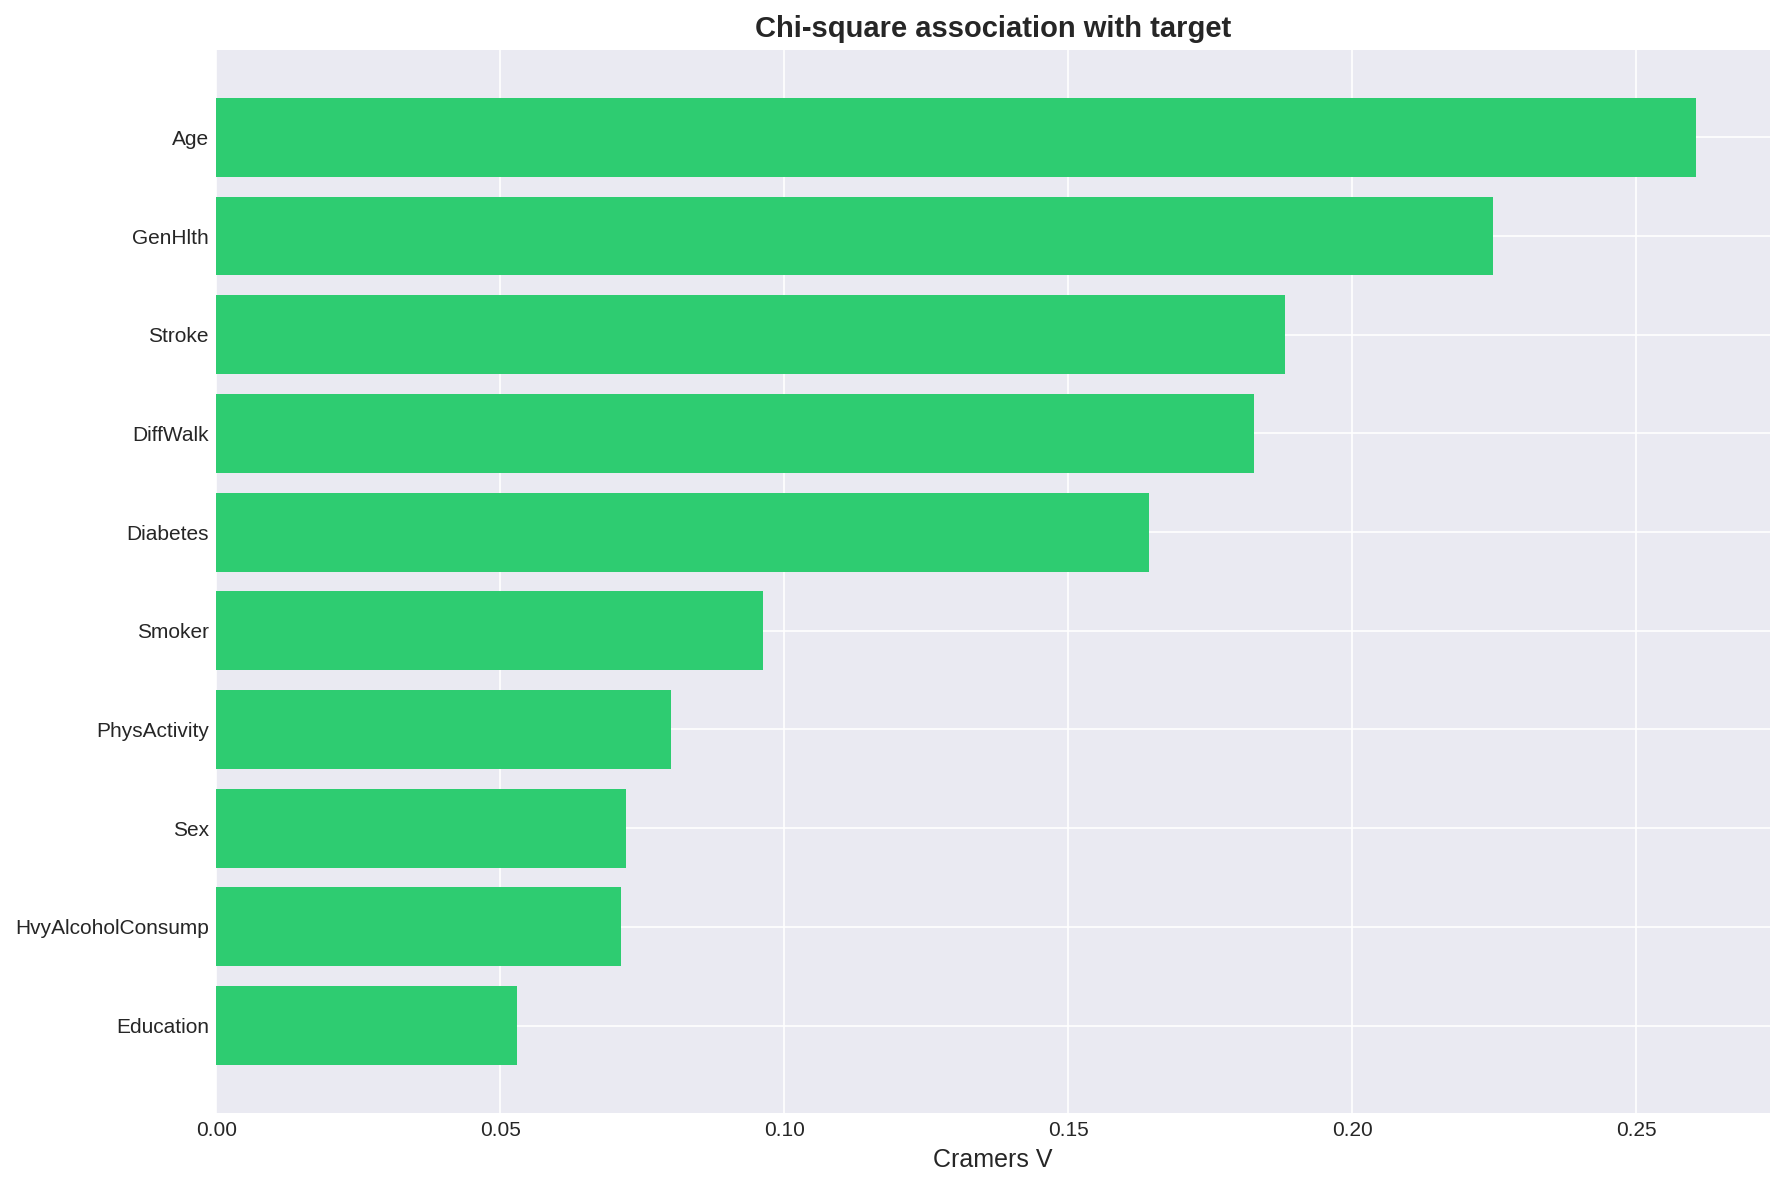
\includegraphics[width=0.80\textwidth]{figures/chi2_cramers_v.png}
    \caption{Association des variables catégorielles avec la variable cible
             (V de Cramér, test du $\chi^2$, $p \ll 0{,}05$ pour toutes les variables).
             Age et GenHlth obtiennent les V de Cramér les plus élevés (0,261 et 0,225),
             en concordance avec l'importance Gini.}
    \label{fig:chi2}
\end{figure}

\subsection{Variables dérivées}

Les deux features composites RiskScore et HealthIndex sont construites selon les
formules~(\ref{eq:riskscore}) et~(\ref{eq:healthindex}) du chapitre~\ref{chap:methodologie}.
Leur distribution selon la classe cible (figure~\ref{fig:derived}) montre une
séparation nette entre les groupes MCV et non-MCV, validant leur apport informatif.

\begin{figure}[H]
    \centering
    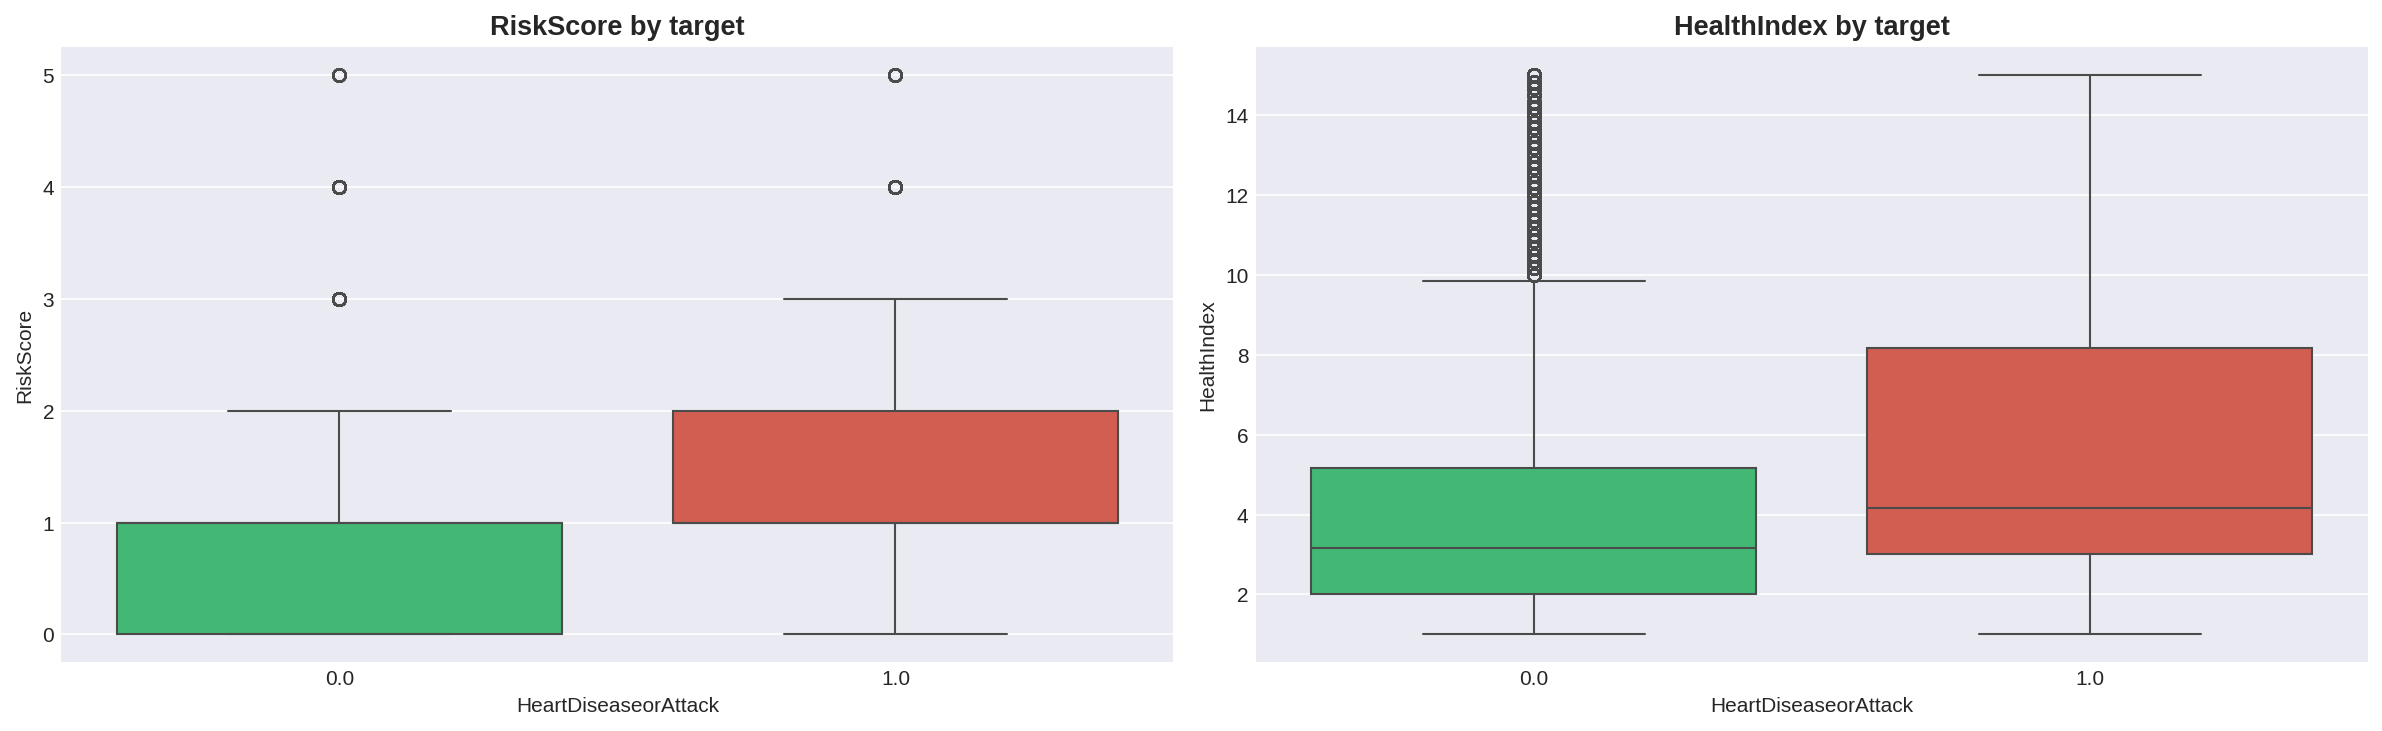
\includegraphics[width=0.90\textwidth]{figures/derived_features.png}
    \caption{Distributions de RiskScore (gauche) et HealthIndex (droite) selon
             la classe cible. Les deux variables présentent une séparation claire~:
             les patients MCV ont en moyenne un RiskScore plus élevé et un HealthIndex
             plus dégradé.}
    \label{fig:derived}
\end{figure}

\subsection{Analyse en composantes principales}

L'ACP est calculée sur les 13 features originales (sans RiskScore ni HealthIndex)
après application d'un filtre de variance (\texttt{VarianceThreshold($10^{-6}$)})
et d'une normalisation StandardScaler. La figure~\ref{fig:pca_analysis} présente
la variance expliquée cumulée par composante principale.

\begin{figure}[H]
    \centering
    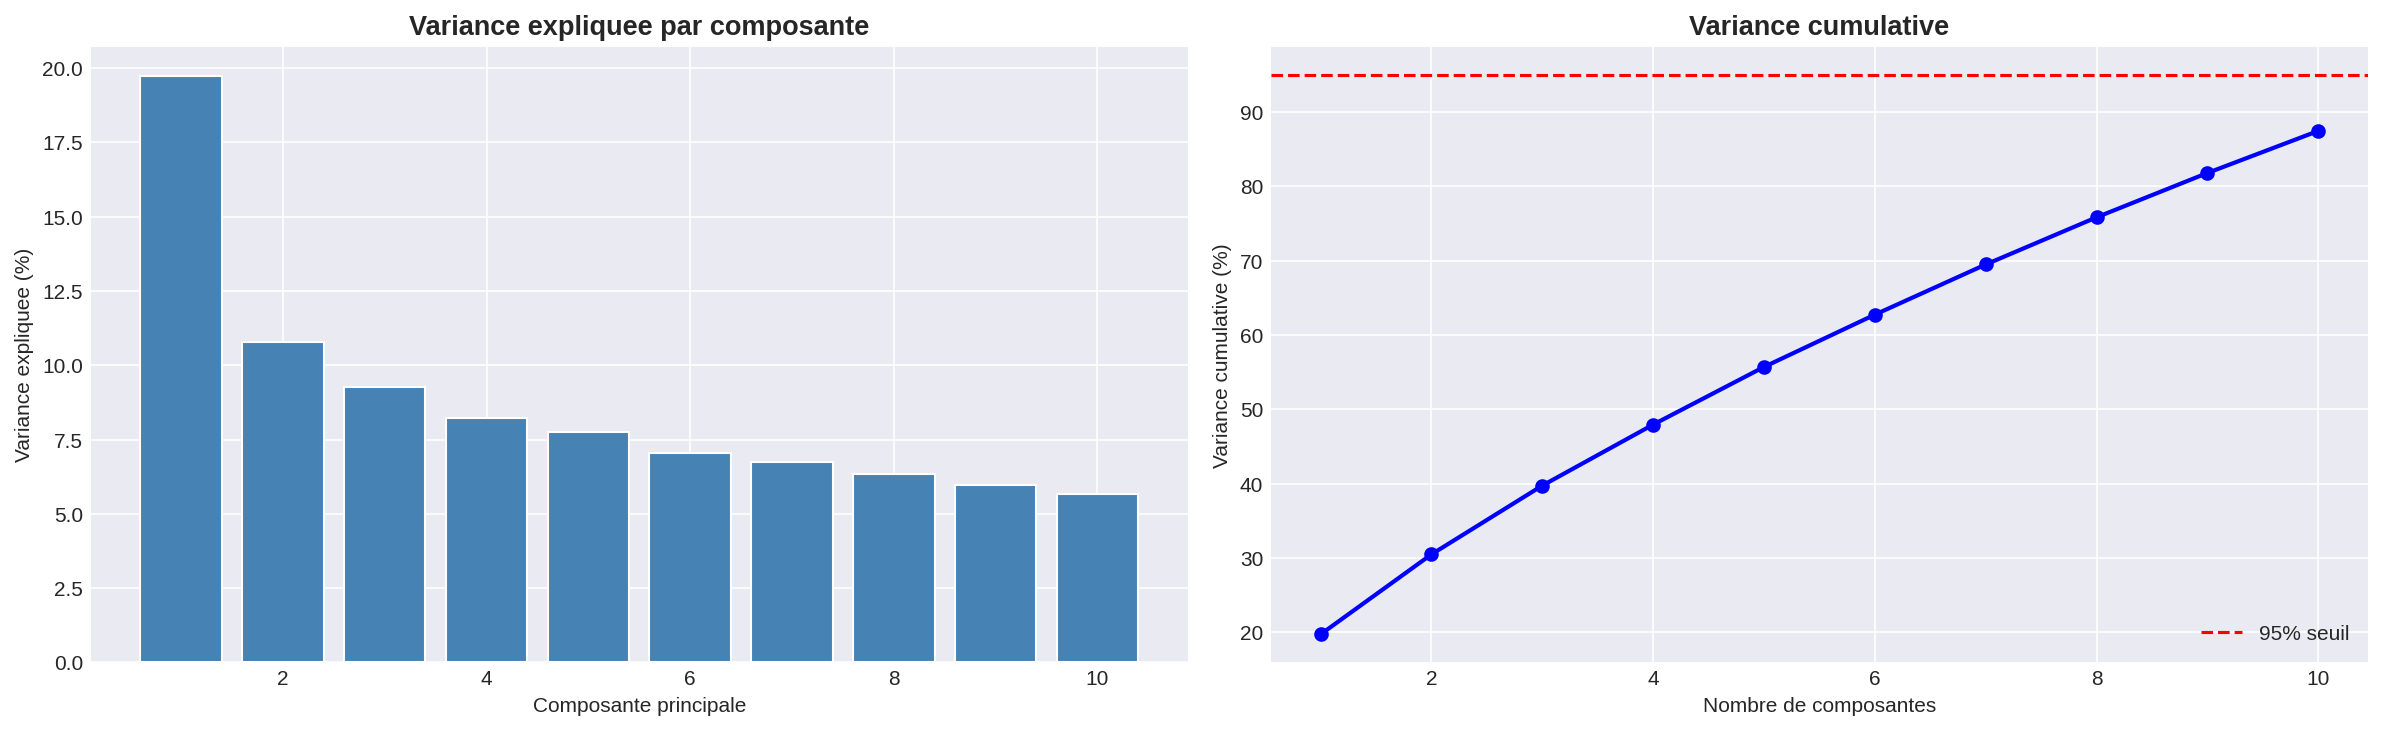
\includegraphics[width=\textwidth]{figures/pca_analysis.png}
    \caption{ACP sur les 13 features originales. Dix composantes expliquent 87,5\%
             de la variance totale. Le seuil de 95\% n'est pas atteint en 10
             composantes, ce qui reflète la nature hétérogène (binaire, ordinale,
             continue) des features BRFSS.}
    \label{fig:pca_analysis}
\end{figure}

La projection en 2D (figure~\ref{fig:pca_2d}) confirme l'absence de séparation
linéaire simple entre les classes, ce qui est cohérent avec un AUC-ROC de 0,82~:
aucune frontière de décision linéaire dans l'espace des deux premières composantes
ne peut atteindre de bonnes performances.

\begin{figure}[H]
    \centering
    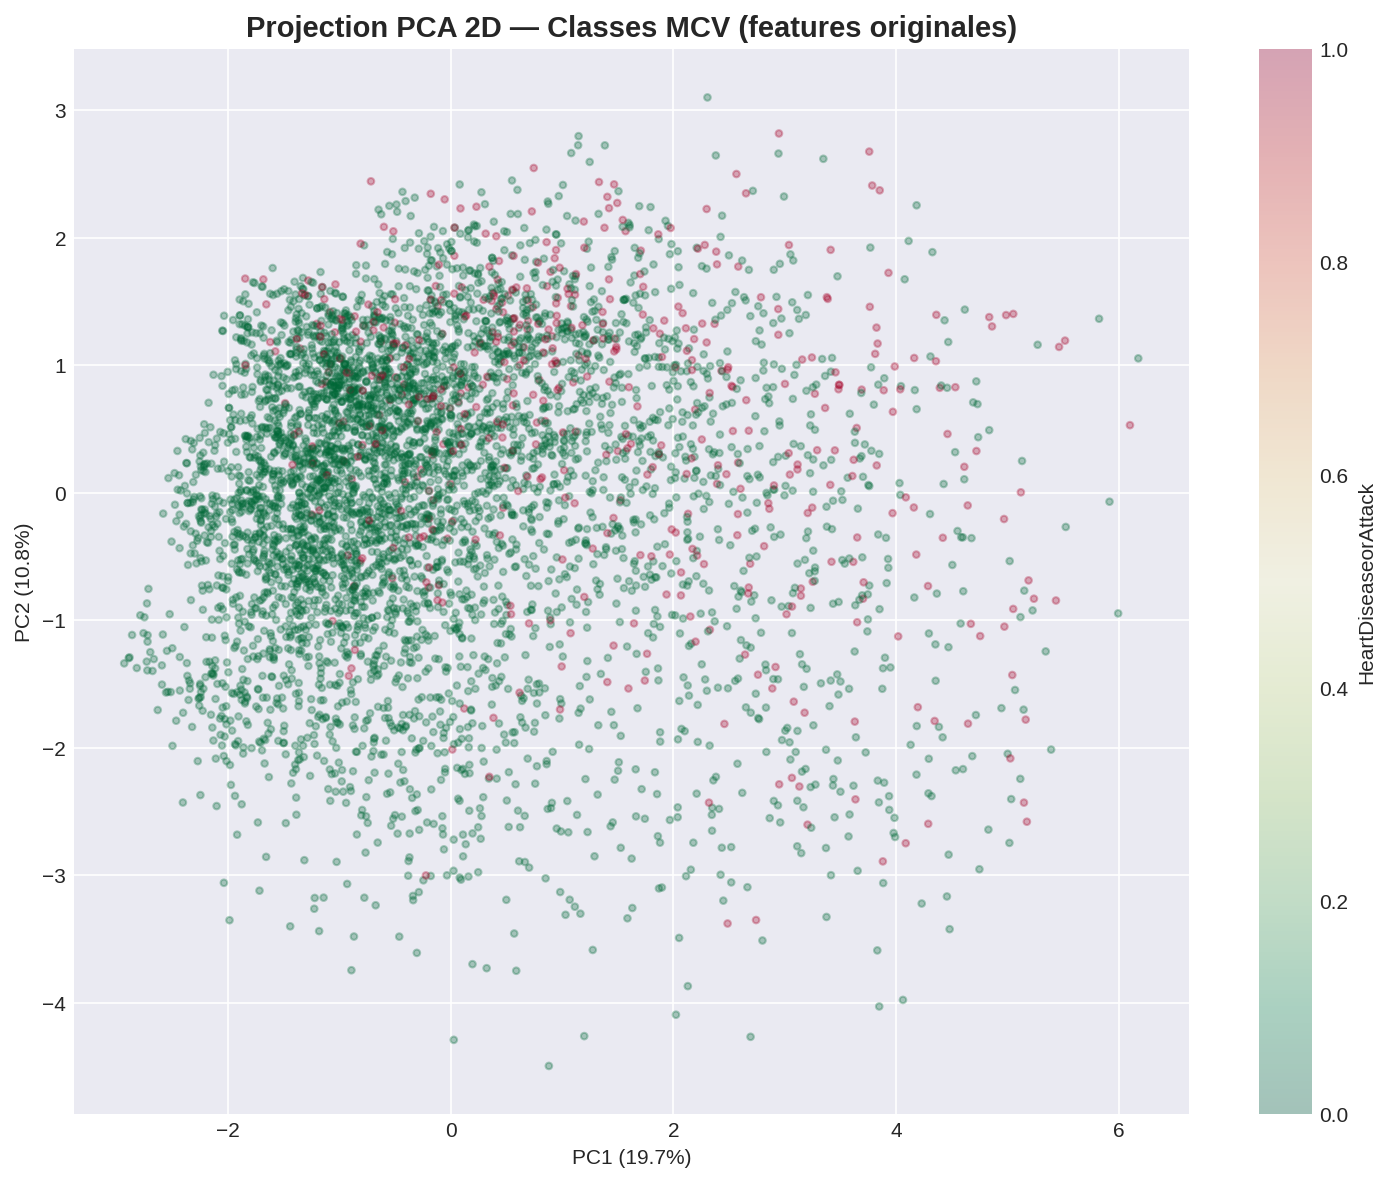
\includegraphics[width=0.60\textwidth]{figures/pca_2d.png}
    \caption{Projection 2D des 13 features originales (PC1 = 19,7\%, PC2 = 10,8\%).
             Les deux classes se superposent largement, justifiant le recours à des
             modèles non linéaires (DNN, XGBoost) plutôt qu'à une régression logistique.}
    \label{fig:pca_2d}
\end{figure}

L'ACP est utilisée exclusivement à titre exploratoire. Le pipeline de modélisation
conserve les 15 features sans réduction de dimension~: DNN et XGBoost traitent
efficacement cet espace, et la réduction de dimension introduirait une perte
d'interprétabilité clinique des features.

% ─────────────────────────────────────────────────────────────────────────────
\section{Phase 4 : Entraînement du réseau de neurones profond}
\label{sec:dnn}
% ─────────────────────────────────────────────────────────────────────────────

\subsection{Partitionnement stratifié et normalisation}

Le jeu de données est partitionné selon un schéma 70/15/15 (entraînement,
validation, test) avec stratification sur la variable cible, maintenant la
prévalence de 10,32\% dans chacune des trois partitions.

Le StandardScaler est ajusté exclusivement sur l'ensemble d'entraînement, puis
appliqué par transformation aux ensembles de validation et de test. Ce protocole
strict prévient toute fuite de données : les statistiques de normalisation
(moyenne, écart-type) ne doivent pas être informées par des exemples du jeu de test.

Les poids de classe sont calculés par la méthode \textit{balanced} sur les étiquettes
de l'ensemble d'entraînement uniquement~: $w_0 = 0{,}558$ (classe négative)
et $w_1 = 4{,}847$ (classe positive).

\subsection{Architecture et entraînement du DNN}

L'architecture du modèle est décrite dans le tableau~\ref{tab:dnn_arch_impl}.
Le réseau est implémenté en TensorFlow 2.19 / Keras~3, avec les composants
de régularisation suivants~:

\begin{table}[H]
\centering
\caption{Architecture du DNN (46\,849 paramètres entraînables)}
\label{tab:dnn_arch_impl}
\begin{tabular}{lrrl}
\toprule
\textbf{Couche} & \textbf{Unités} & \textbf{Paramètres} & \textbf{Remarques} \\
\midrule
Entrée (Dense)      & 256 & 4\,096  & ReLU, $L_2 = 10^{-4}$ \\
Batch Normalization & 256 & 1\,024  & normalisation des activations \\
Dropout             &  -- &     0   & taux = 0,30 \\
Dense               & 128 & 32\,896 & ReLU, $L_2 = 10^{-4}$ \\
Batch Normalization & 128 &   512   & normalisation des activations \\
Dropout             &  -- &     0   & taux = 0,30 \\
Dense               &  64 & 8\,256  & ReLU \\
Sortie (Dense)      &   1 &    65   & Sigmoïde \\
\midrule
\multicolumn{2}{l}{Total paramètres} & 46\,849 & (46\,081 entraînables) \\
\bottomrule
\end{tabular}
\end{table}

Le listing~\ref{lst:dnn_arch} présente la définition de l'architecture en
TensorFlow/Keras, seul extrait de code jugé nécessaire pour illustrer les
choix d'implémentation.

\begin{lstlisting}[caption={Architecture du DNN (TensorFlow 2.19 / Keras 3)},
                   label=lst:dnn_arch]
import tensorflow as tf
from tensorflow.keras import layers, regularizers

def build_dnn(input_dim):
    model = tf.keras.Sequential([
        tf.keras.Input(shape=(input_dim,)),
        layers.Dense(256, activation='relu',
                     kernel_regularizer=regularizers.l2(1e-4)),
        layers.BatchNormalization(),
        layers.Dropout(0.3),
        layers.Dense(128, activation='relu',
                     kernel_regularizer=regularizers.l2(1e-4)),
        layers.BatchNormalization(),
        layers.Dropout(0.3),
        layers.Dense(64, activation='relu'),
        layers.Dense(1, activation='sigmoid')
    ])
    model.compile(
        optimizer=tf.keras.optimizers.Adam(learning_rate=1e-3),
        loss='binary_crossentropy',
        metrics=['accuracy',
                 tf.keras.metrics.AUC(name='auc'),
                 tf.keras.metrics.Precision(name='precision'),
                 tf.keras.metrics.Recall(name='recall')]
    )
    return model
\end{lstlisting}

Deux callbacks contrôlent l'entraînement~: EarlyStopping (patience~=~5, suivi de
val\_auc, avec restauration des meilleurs poids) arrête l'entraînement lorsque
l'AUC de validation cesse de progresser~; ReduceLROnPlateau réduit le taux
d'apprentissage d'un facteur 0,5 lorsque la perte de validation stagne pendant
3 epochs consécutives, jusqu'à un minimum de $10^{-6}$.

L'entraînement s'est déroulé sur 36 epochs (taille de lot 1\,024), le meilleur
modèle ayant été enregistré à l'epoch~31 (val\_auc = 0,8205), pour un temps
total de 177,8~secondes sur deux GPU T4.

\subsection{Optimisation du seuil de classification}

Au seuil par défaut $\tau = 0{,}5$, le DNN avec class weights produit des
probabilités systématiquement plus élevées pour la classe positive, générant
un rappel de 0,80 mais une précision de seulement 0,23. La courbe Précision-Rappel
calculée sur le jeu de test permet d'identifier le seuil $\tau^* = 0{,}6713$,
qui maximise le F1-score en acceptant un rappel réduit (0,56) contre une
précision améliorée (0,30). Ce compromis entre sensibilité et spécificité
est guidé par le contexte clinique~: le seuil 0,5 convient à un outil de
dépistage (maximisation du rappel)~; le seuil 0,67 convient à un outil de
confirmation (minimisation des fausses alertes).

% ─────────────────────────────────────────────────────────────────────────────
\section{Phase 5 : Entraînement XGBoost et benchmark Spark}
% ─────────────────────────────────────────────────────────────────────────────

\subsection{Optimisation des hyperparamètres XGBoost}

XGBoost est entraîné sur les mêmes partitions que le DNN (fichiers \texttt{.npy}
produits à la phase précédente), garantissant la comparabilité des évaluations sur
un jeu de test identique. La méthode de construction d'arbres \texttt{hist}
(histogramme quantilé) est utilisée~: elle est compatible avec l'accélération GPU
et offre des performances supérieures à la méthode exacte pour les grands volumes.

Le paramètre \texttt{scale\_pos\_weight} compense le déséquilibre de classe et est
calculé automatiquement comme $n_{\text{neg}}/n_{\text{pos}} \approx 8{,}69$ sur
l'ensemble d'entraînement. La recherche d'hyperparamètres par RandomizedSearchCV
(20 itérations, 3-fold CV, optimisation sur l'AUC-ROC) a produit les paramètres
optimaux résumés au tableau~\ref{tab:xgb_params_impl}, pour un temps total
de 887~secondes.

\begin{table}[H]
\centering
\caption{Espace de recherche et paramètres optimaux XGBoost}
\label{tab:xgb_params_impl}
\begin{tabular}{lll}
\toprule
\textbf{Hyperparamètre} & \textbf{Espace de recherche} & \textbf{Valeur optimale} \\
\midrule
n\_estimators      & \{300, 400, 500\}              & 400  \\
max\_depth         & \{4, 5, 6, 7\}                 & 5    \\
learning\_rate     & \{0,01, 0,05, 0,1\}            & 0,05 \\
subsample          & \{0,7, 0,8, 0,9\}              & 0,8  \\
colsample\_bytree  & \{0,7, 0,8, 0,9\}              & 0,7  \\
min\_child\_weight & \{1, 3, 5, 7\}                 & 3    \\
gamma              & \{0, 0,1, 0,2\}                & 0,1  \\
scale\_pos\_weight & $n_{\text{neg}}/n_{\text{pos}} \approx 8{,}69$ & 8,69 \\
\bottomrule
\end{tabular}
\end{table}

\subsection{GBTClassifier Spark MLlib}

Le GBTClassifier de Spark MLlib est entraîné sur une partition 85\%/15\% issue
du fichier Parquet complet via \texttt{randomSplit}, sans stratification. Cette
partition légèrement différente (264\,632 lignes de test contre 264\,037 pour
DNN/XGBoost) est inhérente à l'API Spark et explique les minimes variations entre
les ensembles de test. La configuration retenue comprend 100 arbres, une profondeur
maximale de 6 et un pas d'apprentissage de 0,1~; le temps d'entraînement est
de 270,2~secondes.

Il est important de noter que la métrique F1 pondérée de Spark (0,860) n'est
pas comparable aux F1 binaires de la classe positive rapportés pour le DNN et
XGBoost~: dominé à 89,7\% par la classe négative, ce score reflète principalement
la performance sur la classe majoritaire. La comparaison inter-modèles s'appuie
donc exclusivement sur l'AUC-ROC.

\subsection{Benchmark temporel Spark vs. XGBoost standalone}

Un benchmark contrôlé mesure le temps d'entraînement d'un modèle réduit
(50 arbres, profondeur 5) sur cinq fractions croissantes du jeu de données
(10\% à 100\%, soit de 149\,510 à 1\,495\,609 lignes), en alternant
Spark GBTClassifier et XGBoost standalone. La figure~\ref{fig:scalability}
présente les résultats de ce benchmark.

\begin{figure}[H]
    \centering
    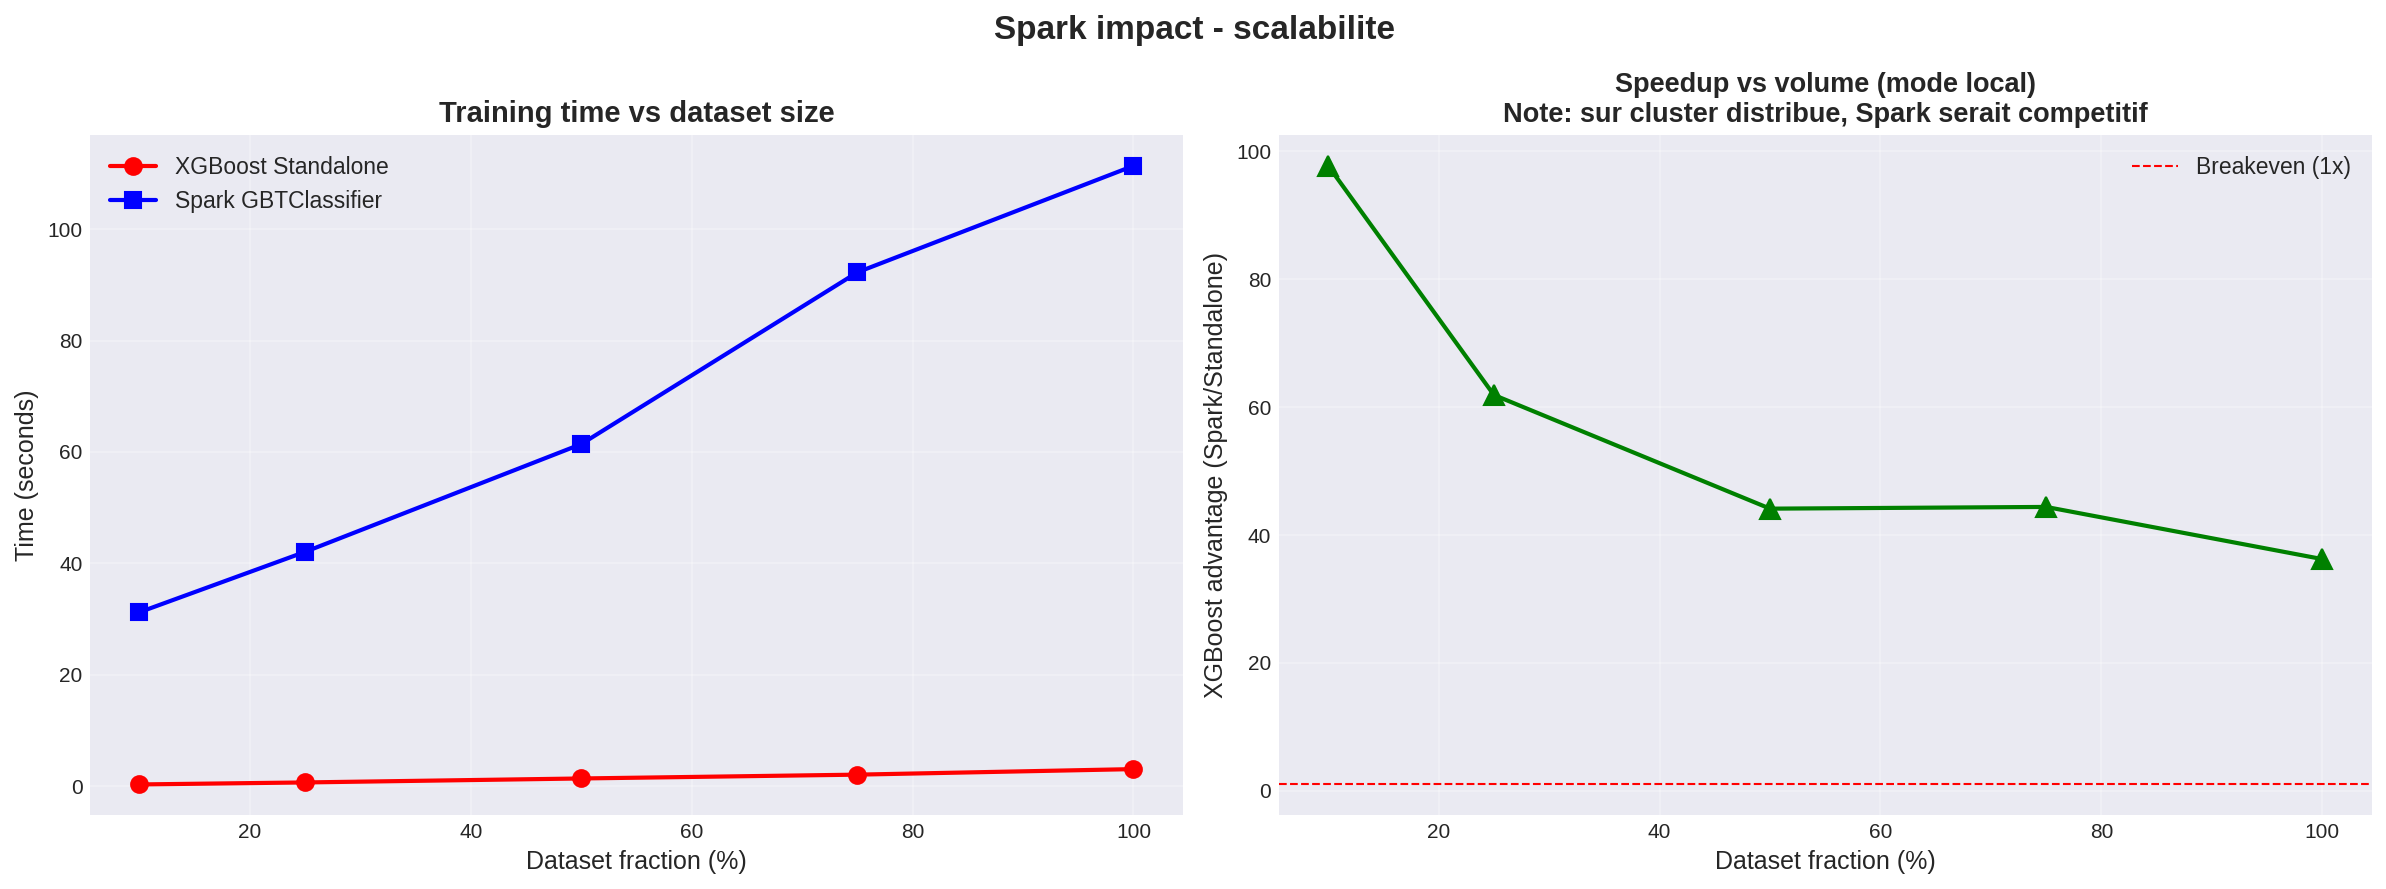
\includegraphics[width=\textwidth]{figures/spark_scalability.png}
    \caption{Comparaison des temps d'entraînement Spark GBT et XGBoost standalone
             en fonction de la taille du jeu de données (gauche), et facteur
             d'avantage XGBoost correspondant (droite). En mode local sur
             une seule machine, XGBoost est 36 à 98 fois plus rapide que Spark GBT.}
    \label{fig:scalability}
\end{figure}

L'écart observé (36 à 97 fois) traduit l'overhead inhérent à Spark en mode local~:
sérialisation des données, communication entre le pilote et les exécuteurs,
et démarrage de la JVM. Sur un cluster distribué de huit nœuds ou plus,
Spark deviendrait compétitif pour des volumes dépassant 10~millions de lignes,
conformément aux résultats publiés par Zhang et al.~\cite{zhang2023}.

% ─────────────────────────────────────────────────────────────────────────────
\section{Phase 6 : Tableau de bord Streamlit}
% ─────────────────────────────────────────────────────────────────────────────

Le tableau de bord Streamlit est une application multi-pages découplée du pipeline
d'entraînement. Elle charge des artefacts pré-calculés (fichiers JSON, CSV et PNG)
depuis un dossier \texttt{results/} et peut être exécutée localement sans Spark ni
modèle chargé en mémoire. L'application est structurée en une page d'accueil et
trois pages d'analyse thématiques.

\subsection{Page d'accueil}

La page d'accueil (figure~\ref{fig:streamlit_home}) présente les quatre indicateurs
clés du projet~: nombre total d'observations, nombre de variables, prévalence MCV
et meilleur AUC-ROC obtenu. Elle donne également un aperçu de la stack technique et
oriente l'utilisateur vers les trois pages d'analyse via le menu latéral.

\begin{figure}[H]
    \centering
    \includegraphics[width=\textwidth]{figures/streamlit_accueil.png}
    \caption{Page d'accueil du tableau de bord Streamlit --- indicateurs clés du
             projet (observations, variables, prévalence MCV, AUC-ROC) et
             description de la stack technique.}
    \label{fig:streamlit_home}
\end{figure}

\subsection{Page EDA — Exploration des données}

La page EDA (figure~\ref{fig:streamlit_eda}) permet d'explorer interactivement
le dataset BRFSS sur un échantillon de 100\,000 lignes. Elle propose~:
\begin{itemize}
    \item des filtres latéraux par sexe et tranche d'âge appliqués dynamiquement ;
    \item la distribution de la variable cible (camembert et histogramme) ;
    \item les distributions univariées de chaque feature par classe (MCV / non-MCV) ;
    \item les matrices de corrélation de Pearson et Spearman et l'évolution du taux
          de MCV par tranche d'âge.
\end{itemize}

\begin{figure}[H]
    \centering
    \includegraphics[width=\textwidth]{figures/streamlit_eda.png}
    \caption{Page EDA du tableau de bord --- exploration interactive des distributions
             du dataset BRFSS 2020--2024 avec filtres par sexe et tranche d'âge.}
    \label{fig:streamlit_eda}
\end{figure}

\subsection{Page Résultats des modèles}

La page Résultats (figure~\ref{fig:streamlit_models}) compare les performances
du DNN et d'XGBoost via~:
\begin{itemize}
    \item un sélecteur de seuil DNN (optimal F1 ou défaut 0,5) dans la barre latérale ;
    \item cinq indicateurs KPI (accuracy, précision, rappel, F1-score, AUC-ROC) ;
    \item les courbes ROC superposées, les matrices de confusion et le graphique
          d'impact du seuil sur les métriques ;
    \item les importances de features XGBoost (critères weight, gain et cover).
\end{itemize}

\begin{figure}[H]
    \centering
    \includegraphics[width=\textwidth]{figures/streamlit_models.png}
    \caption{Page Résultats des modèles --- comparaison DNN vs XGBoost avec
             sélecteur de seuil interactif, courbes ROC et matrices de confusion.}
    \label{fig:streamlit_models}
\end{figure}

\subsection{Page Impact Spark}

La page Impact Spark (figure~\ref{fig:streamlit_spark}) présente~:
\begin{itemize}
    \item les temps d'entraînement des trois modèles (DNN, XGBoost, Spark GBT)
          sous forme de KPI et d'histogramme~;
    \item le graphique de scalabilité Spark vs XGBoost standalone sur cinq fractions
          croissantes du dataset~;
    \item le facteur d'avantage XGBoost (36 à 97 fois) en fonction du volume~;
    \item une synthèse de la valeur ajoutée de Spark dans chaque phase du pipeline.
\end{itemize}

\begin{figure}[H]
    \centering
    \includegraphics[width=\textwidth]{figures/streamlit_spark.png}
    \caption{Page Impact Spark --- benchmark XGBoost standalone vs Spark GBTClassifier
             sur cinq fractions du jeu de données (10\% à 100\%), avec facteur
             d'avantage et analyse de la valeur ajoutée du traitement distribué.}
    \label{fig:streamlit_spark}
\end{figure}

Les chemins de fichiers sont résolus de façon portable via \texttt{Path(\_\_file\_\_).parent},
et les fonctions de chargement gèrent les fichiers manquants par un avertissement
non bloquant, garantissant la robustesse de l'application en cas de résultats
partiels. L'application est lancée par la commande \texttt{streamlit run app.py}
depuis le dossier \texttt{streamlit\_dashboard/}.

\chapter{Résultats et Discussion}
\label{chap:resultats}

% ─────────────────────────────────────────────────────────────────────────────
\section{Résultats de l'analyse exploratoire (EDA)}
% ─────────────────────────────────────────────────────────────────────────────

\subsection{Statistiques descriptives du dataset nettoyé}

Après l'étape de binarisation BRFSS et de déduplication, le dataset présente
les statistiques descriptives du tableau~\ref{tab:stats_eda}.

\begin{table}[H]
\centering
\caption{Statistiques descriptives du dataset nettoyé (n = 1\,760\,241)}
\label{tab:stats_eda}
\begin{tabular}{lrrrrr}
\toprule
\textbf{Variable} & \textbf{Moyenne} & \textbf{Médiane} & \textbf{Écart-type} & \textbf{Min} & \textbf{Max} \\
\midrule
BMI            & 28,38 &  27,54 &  6,25 & 12,0 & 98,0 \\
GenHlth        &  2,52 &   2,00 &  1,09 &  1,0 &  5,0 \\
Age            &  8,42 &   9,00 &  2,87 &  1,0 & 13,0 \\
MentHlth       &  3,47 &   0,00 &  7,89 &  0,0 & 30,0 \\
PhysHlth       &  4,56 &   0,00 &  9,12 &  0,0 & 30,0 \\
RiskScore      &  0,82 &   1,00 &  0,91 &  0,0 &  5,0 \\
HealthIndex    &  4,02 &   3,33 &  2,21 &  1,0 & 15,0 \\
\bottomrule
\end{tabular}
\end{table}

La médiane de MentHlth et PhysHlth est égale à 0~: la majorité des répondants
déclarent aucun jour de mauvaise santé dans les 30 jours précédents, produisant
des distributions fortement asymétriques à droite. Ce comportement est cohérent
avec la littérature épidémiologique BRFSS et ne constitue pas une anomalie de données.

\subsection{Distributions univariées}

La figure~\ref{fig:univariate} présente les distributions de l'ensemble des features
numériques et ordinales, comparées entre la classe MCV (positif) et la classe
non-MCV (négatif). Cette visualisation permet d'identifier visuellement les features
les plus discriminantes avant toute modélisation.

\begin{figure}[H]
    \centering
    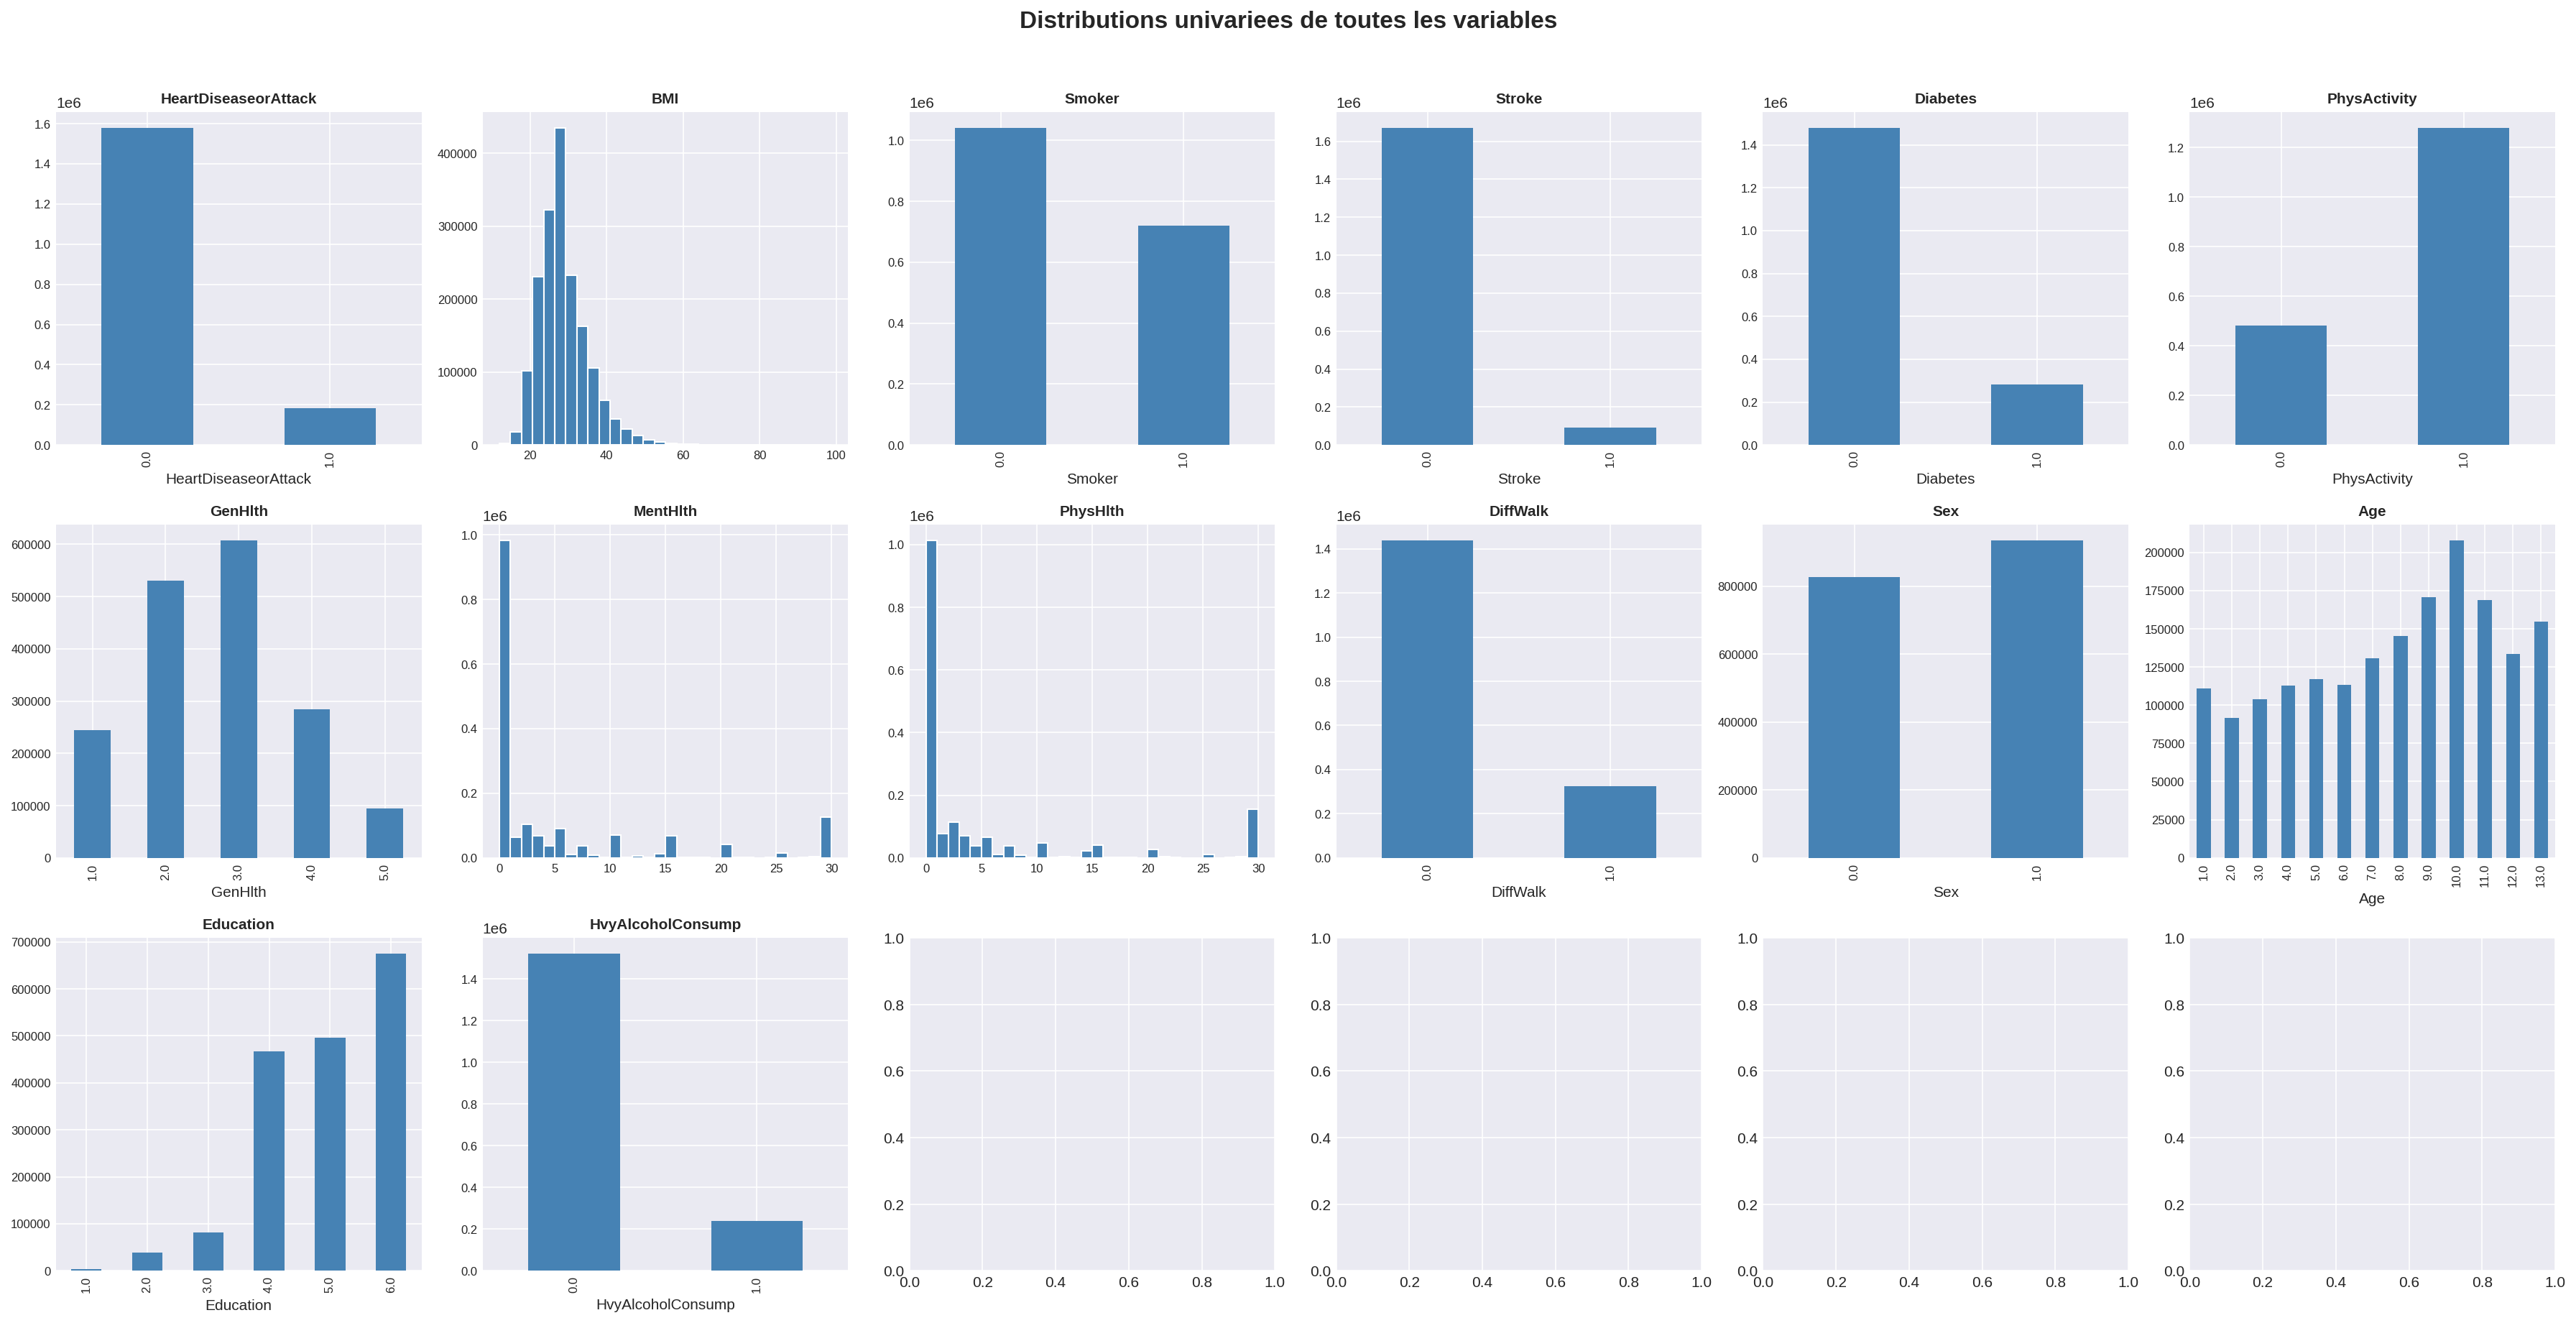
\includegraphics[width=\textwidth]{figures/univariate_distributions.png}
    \caption{Distributions univariées des features numériques et ordinales selon
             la classe cible (bleu~: non-MCV, orange~: MCV). Age, GenHlth et Stroke
             présentent les décalages les plus marqués entre classes,
             confirmant leur pouvoir discriminant.}
    \label{fig:univariate}
\end{figure}

Les observations principales sont les suivantes~:
\begin{itemize}
    \item \textbf{Age}~: les patients MCV se concentrent dans les tranches 9--13
          (55 ans et plus), avec une médiane supérieure d'environ 2 tranches
          par rapport aux non-MCV.
    \item \textbf{GenHlth}~: les patients MCV s'auto-évaluent en moins bonne santé
          (distribution décalée vers les valeurs 3--5).
    \item \textbf{BMI}~: légère différence de distribution, les MCV ayant un BMI
          médian légèrement plus élevé, mais les distributions se chevauchent
          fortement, limitant le pouvoir discriminant de cette variable seule.
\end{itemize}

\subsection{Distribution de la variable cible}

La figure~\ref{fig:target_dist} illustre le déséquilibre de classes dans le dataset
nettoyé. La classe positive (MCV diagnostiquée) représente 10,32\% des observations.

\begin{figure}[H]
    \centering
    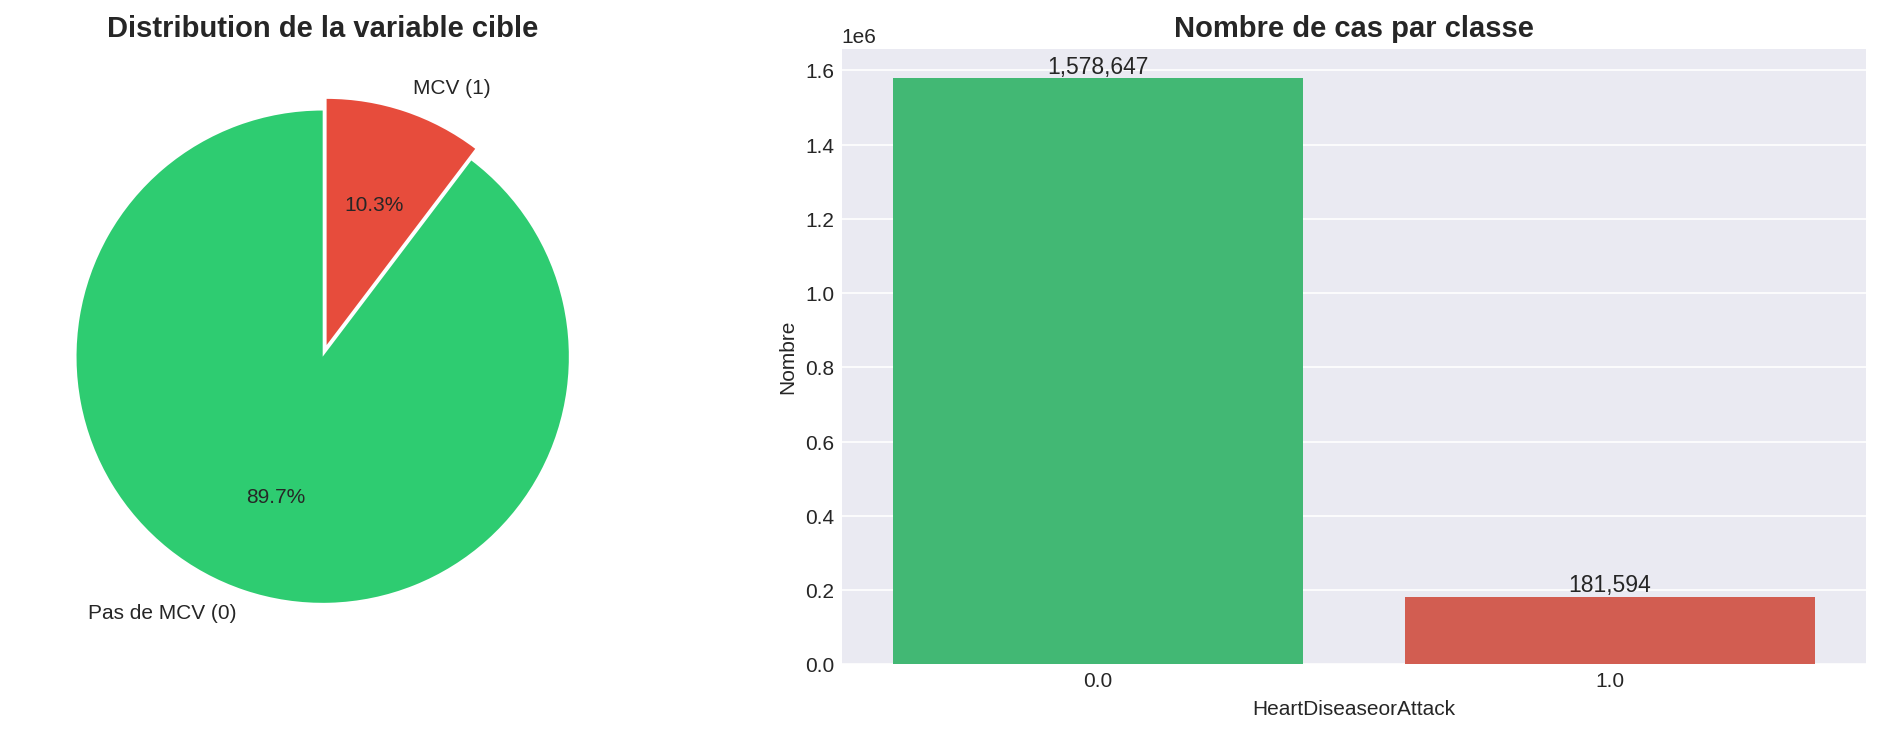
\includegraphics[width=0.75\textwidth]{figures/target_distribution.png}
    \caption{Distribution de la variable cible \texttt{HeartDiseaseorAttack}
             après nettoyage (1\,760\,241 observations). Le rapport de classes
             8,68~:~1 est inhérent à la prévalence épidémiologique réelle des MCV
             dans la population américaine adulte.}
    \label{fig:target_dist}
\end{figure}

\subsection{Analyse des corrélations}

La figure~\ref{fig:corr} présente la matrice de corrélation de Pearson sur
l'ensemble des features. Les corrélations positives les plus fortes avec la cible
sont observées pour Age (0,250), GenHlth (0,213), Stroke (0,188) et DiffWalk (0,183).
La corrélation négative la plus marquée concerne PhysActivity ($-$0,094),
confirmant l'effet protecteur de l'activité physique.

\begin{figure}[H]
    \centering
    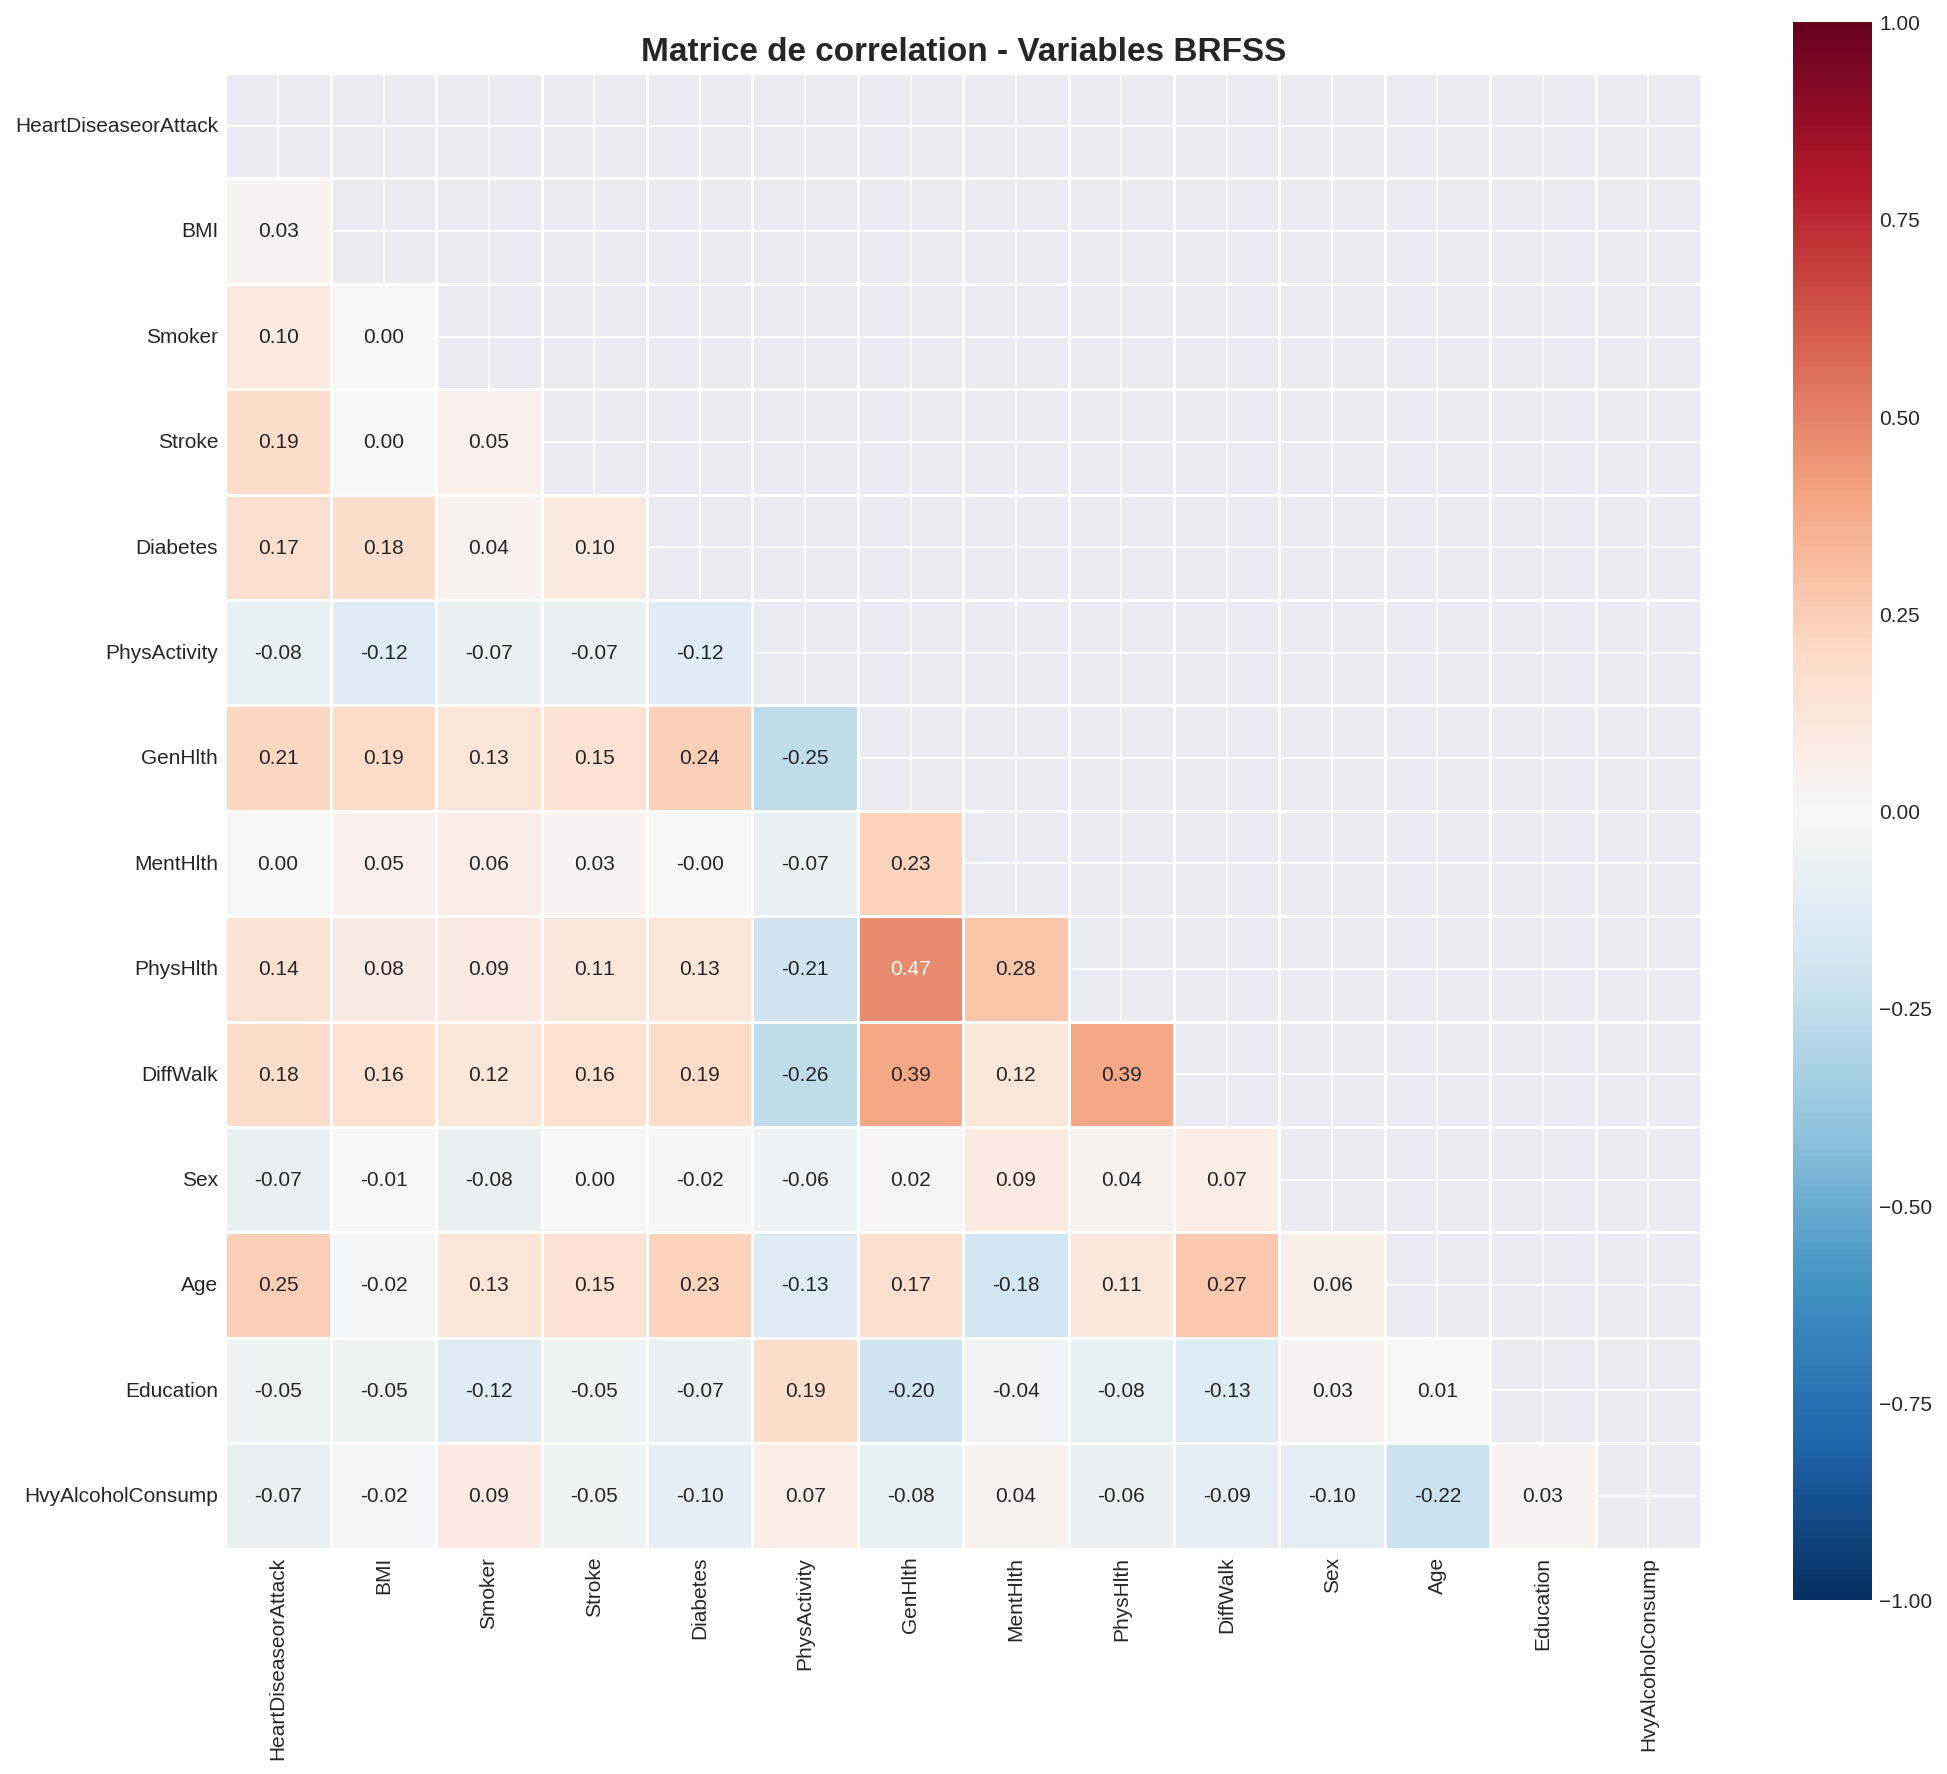
\includegraphics[width=\textwidth]{figures/correlation_heatmap.png}
    \caption{Matrice de corrélation de Pearson — dataset BRFSS 2020--2024 (n = 200\,000).
             Les corrélations entre features restent modérées (pas de multi-colinéarité
             sévère), la corrélation maximale entre prédicteurs est de 0,32
             (entre RiskScore et Stroke, attendue par construction).}
    \label{fig:corr}
\end{figure}

La figure~\ref{fig:target_correlation} compare les corrélations de chaque feature
avec la variable cible, en regard de l'importance Gini, pour mettre en évidence
les convergences et divergences entre les deux méthodes d'évaluation.

\begin{figure}[H]
    \centering
    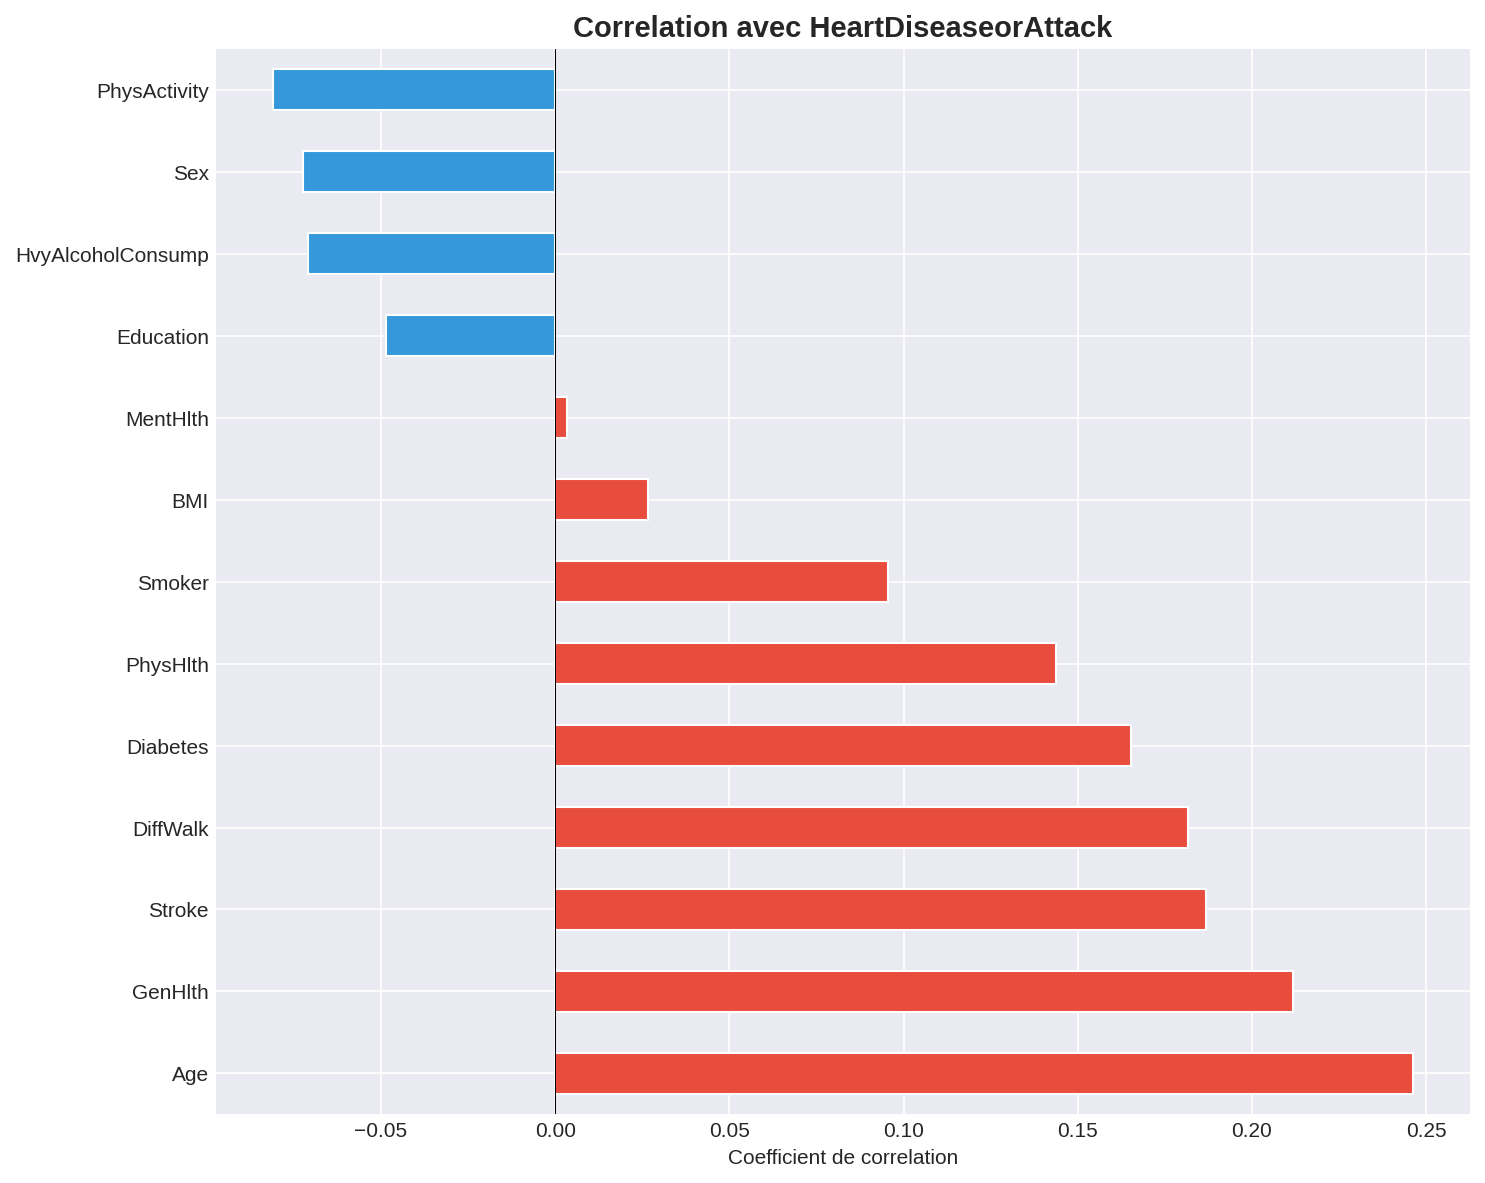
\includegraphics[width=0.85\textwidth]{figures/target_correlation.png}
    \caption{Corrélation de chaque feature avec la variable cible (axe horizontal)
             versus son importance Gini normalisée (axe vertical).
             Les features proches de la diagonale sont cohérentes entre les deux
             méthodes~; les divergences notables concernent BMI (Gini élevé,
             corrélation faible) et PhysActivity (corrélation élevée, Gini faible).}
    \label{fig:target_correlation}
\end{figure}

\subsection{Importance des features}

La figure~\ref{fig:gini} présente l'importance Gini calculée par un Random Forest
préliminaire de 100 arbres. Les trois features dominantes sont~: Age (34,06\%),
GenHlth (20,33\%) et Stroke (16,13\%), représentant à elles seules 70,5\%
de l'importance totale.

\begin{figure}[H]
    \centering
    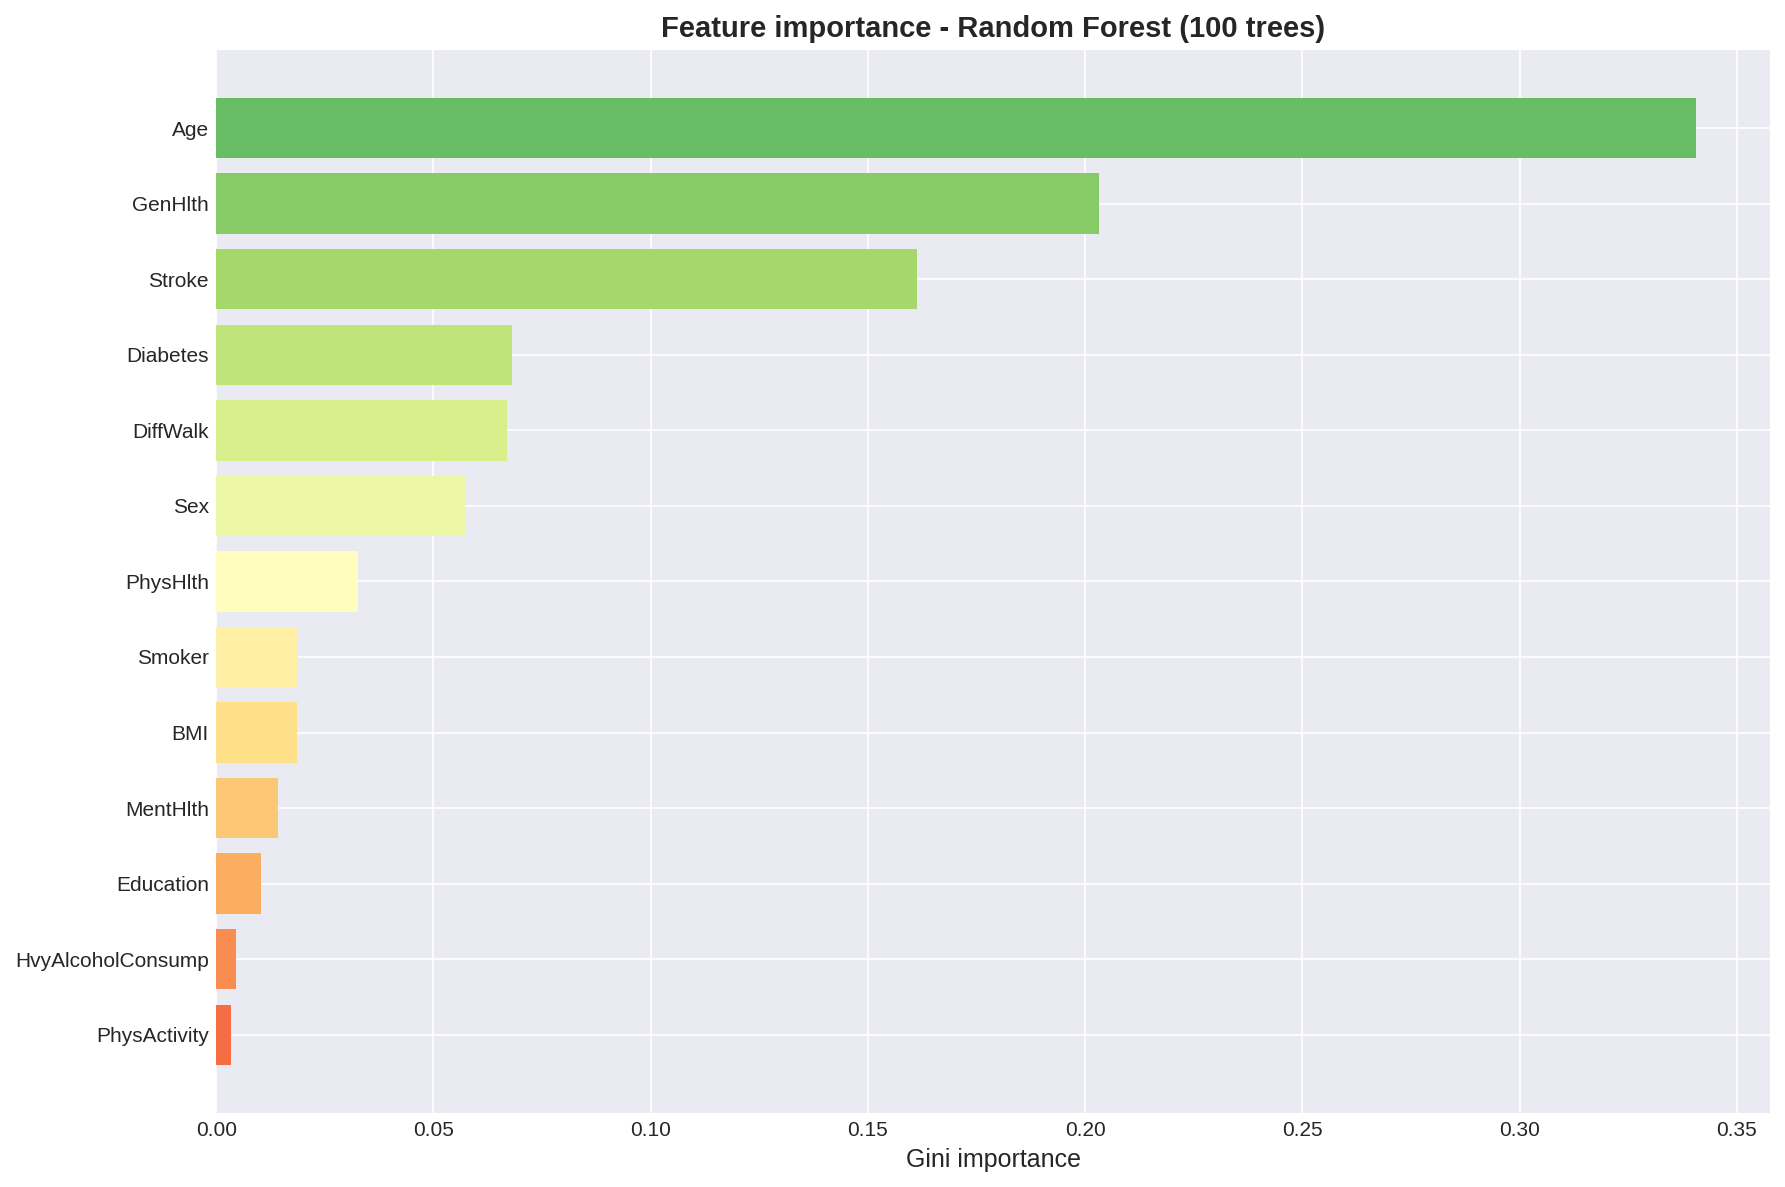
\includegraphics[width=0.85\textwidth]{figures/feature_importance_gini.png}
    \caption{Importance des features par critère de réduction d'impureté de Gini
             (Random Forest, 100 arbres, 30\% de l'échantillon). Age, GenHlth et
             Stroke dominent avec 70,5\% de l'importance totale, cohérent avec
             la littérature épidémiologique sur les facteurs de risque cardiovasculaire.}
    \label{fig:gini}
\end{figure}

% ─────────────────────────────────────────────────────────────────────────────
\section{Performances des modèles}
% ─────────────────────────────────────────────────────────────────────────────

\subsection{Comparaison globale des métriques}

\begin{table}[H]
\centering
\caption{Comparaison des performances sur le jeu de test --- DNN vs XGBoost vs Spark GBT}
\label{tab:results_comparison}
\begin{tabular}{lcccc}
\toprule
\textbf{Métrique} & \textbf{DNN ($\tau=0{,}5$)} & \textbf{DNN ($\tau=0{,}67$)} & \textbf{XGBoost} & \textbf{Spark GBT} \\
\midrule
Accuracy           & 0,698 & 0,822 & 0,701 & 0,898 \\
Précision          & 0,227 & 0,305 & 0,229 & --- \\
Rappel             & 0,802 & 0,563 & 0,799 & --- \\
F1-Score           & 0,354 & 0,396 & 0,356 & 0,860\textsuperscript{*} \\
AUC-ROC            & \multicolumn{2}{c}{0,819} & 0,820 & 0,819 \\
Temps entraîn.~(s) & \multicolumn{2}{c}{177,8} & 67,1  & 270,2 \\
Temps inférence~(s)& \multicolumn{2}{c}{0,93}  & 1,51  & 0,05 \\
\bottomrule
\multicolumn{5}{l}{\textsuperscript{*} F1 pondéré (weighted), dominé par la classe négative
                    — non comparable aux F1 binaires}
\end{tabular}
\end{table}

Les figures~\ref{fig:metrics_barchart} et~\ref{fig:metrics_radar} comparent
graphiquement les métriques des modèles sous deux représentations complémentaires.

\begin{figure}[H]
    \centering
    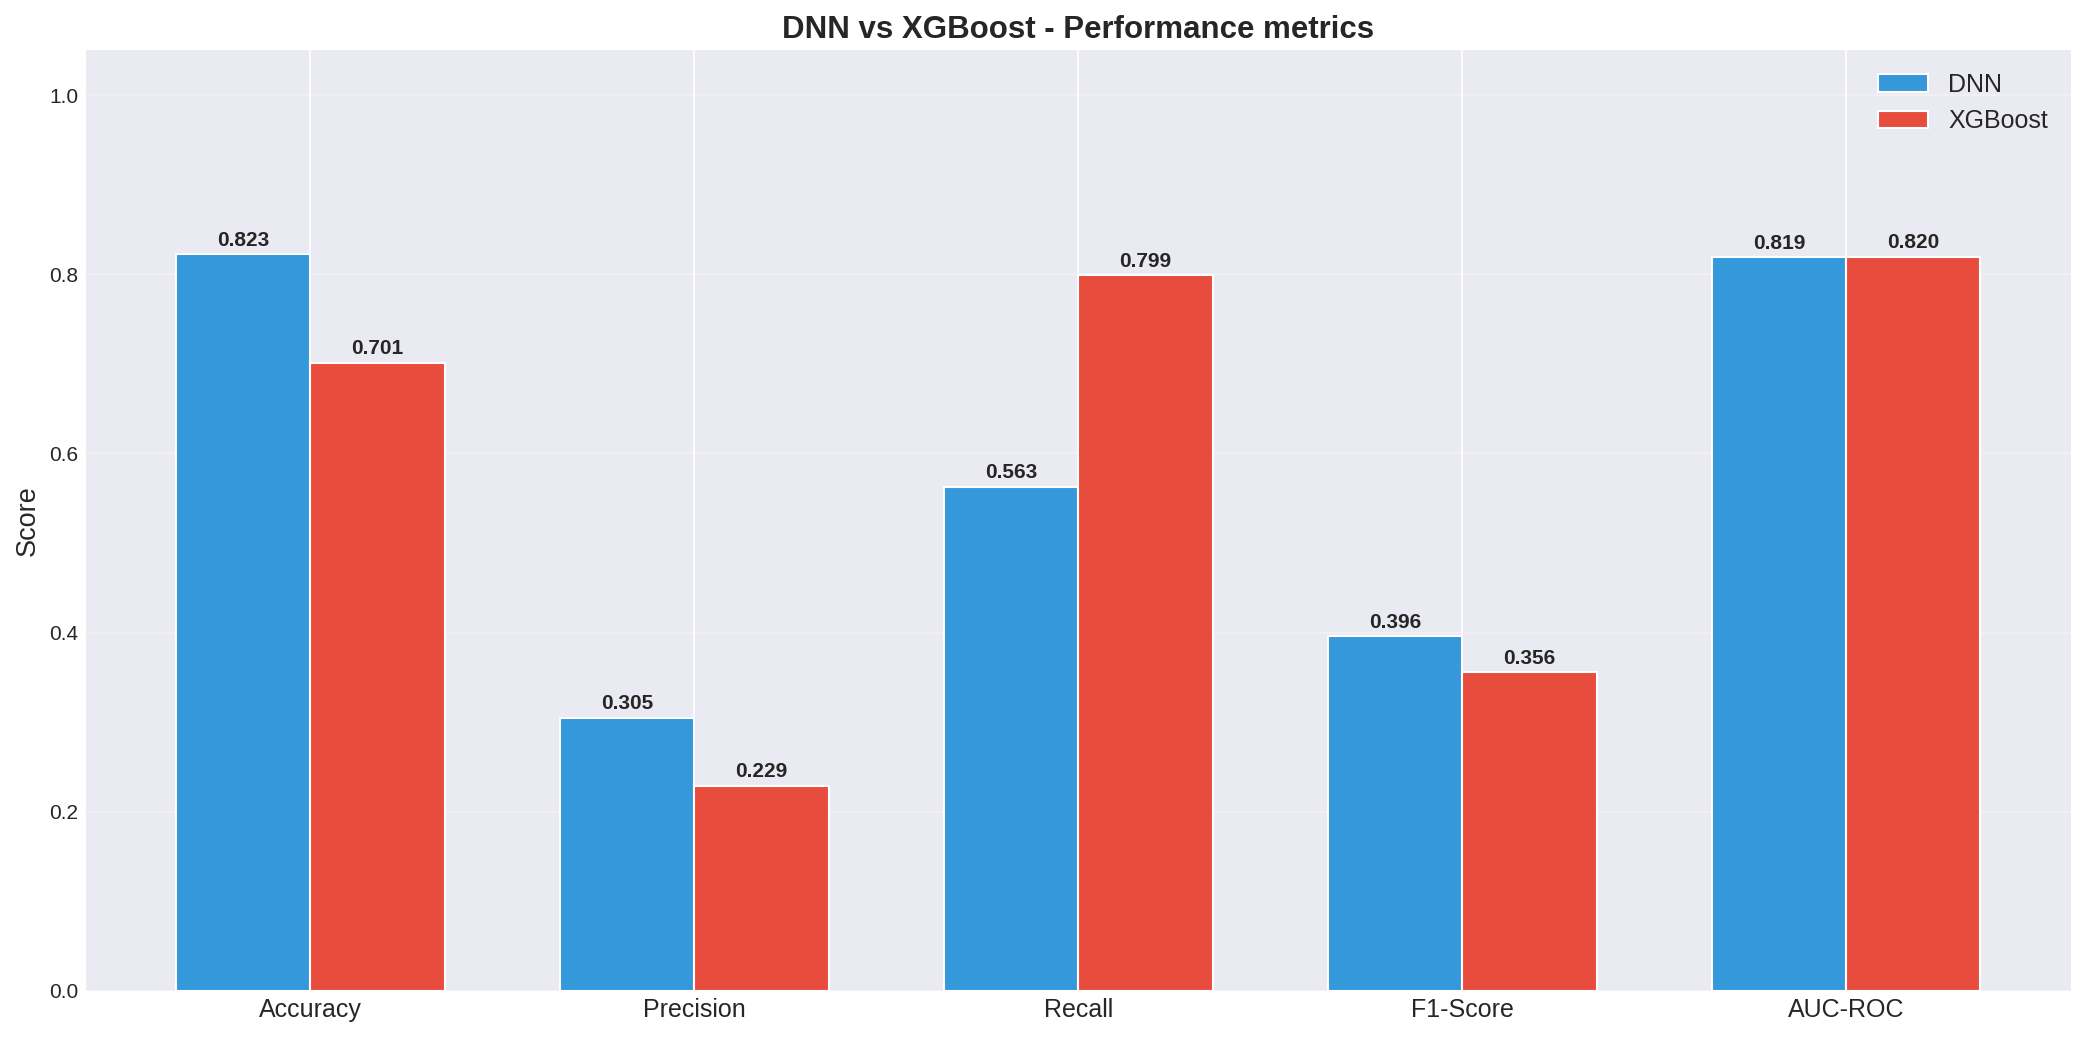
\includegraphics[width=\textwidth]{figures/metrics_comparison_barchart.png}
    \caption{Comparaison des métriques par histogramme pour DNN (seuil 0,5),
             DNN (seuil 0,67) et XGBoost. L'AUC-ROC converge vers 0,82 pour
             les trois modèles, tandis que le rappel et la précision varient
             selon le seuil choisi.}
    \label{fig:metrics_barchart}
\end{figure}

\begin{figure}[H]
    \centering
    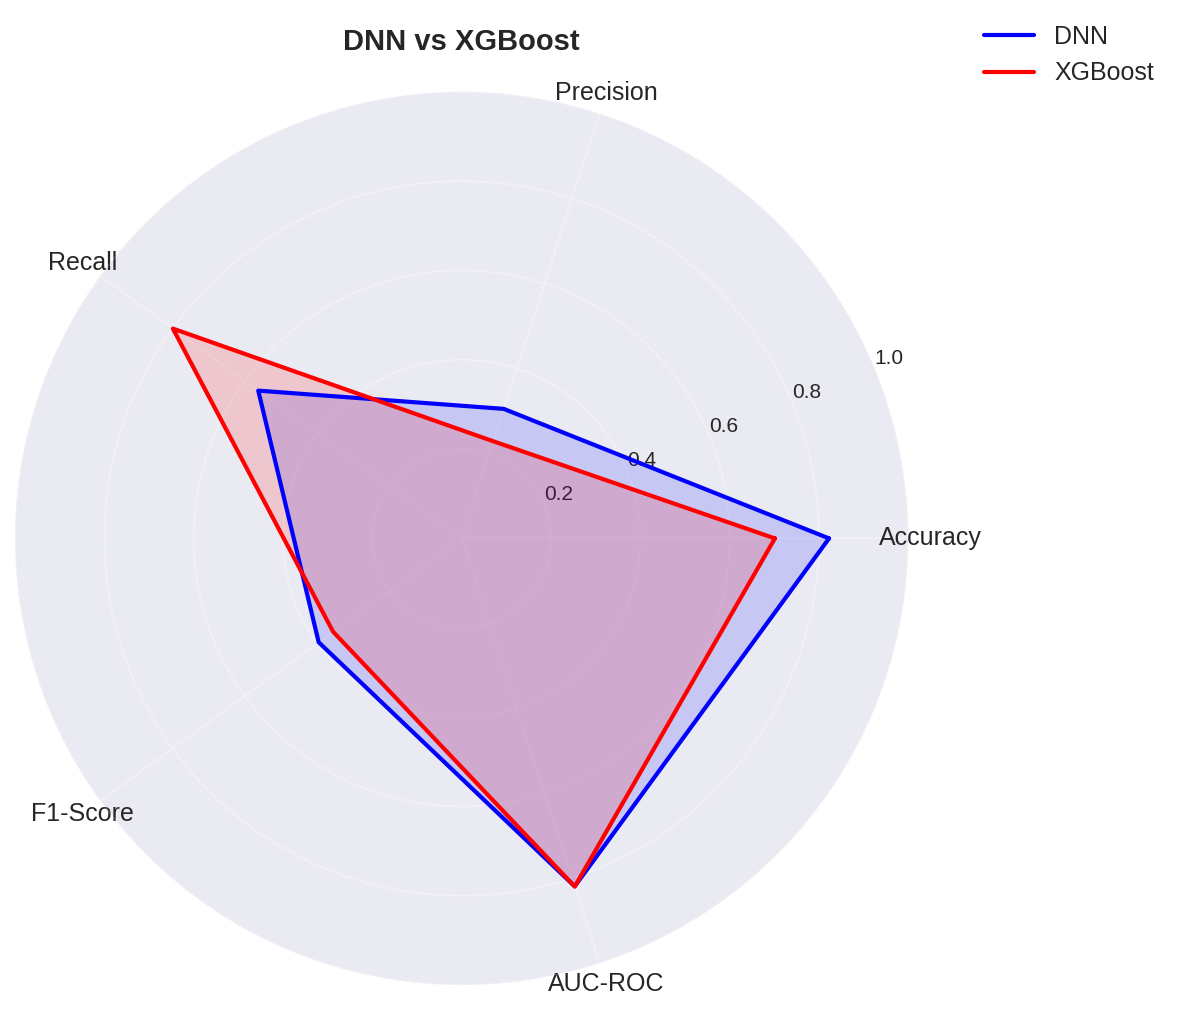
\includegraphics[width=0.70\textwidth]{figures/metrics_radar_chart.png}
    \caption{Graphique radar des métriques comparatives (accuracy, précision,
             rappel, F1-score, AUC-ROC). XGBoost au seuil 0,5 présente le
             meilleur rappel (79,9\%), tandis que DNN au seuil 0,67 offre
             le meilleur compromis précision-rappel (F1 = 0,396).}
    \label{fig:metrics_radar}
\end{figure}

\subsection{Résultats détaillés du DNN}

La figure~\ref{fig:dnn_roc} présente la courbe ROC du DNN, et la figure~\ref{fig:dnn_cm}
sa matrice de confusion au seuil optimal de 0,6713.

\begin{figure}[H]
    \centering
    \begin{subfigure}[b]{0.48\textwidth}
        \centering
        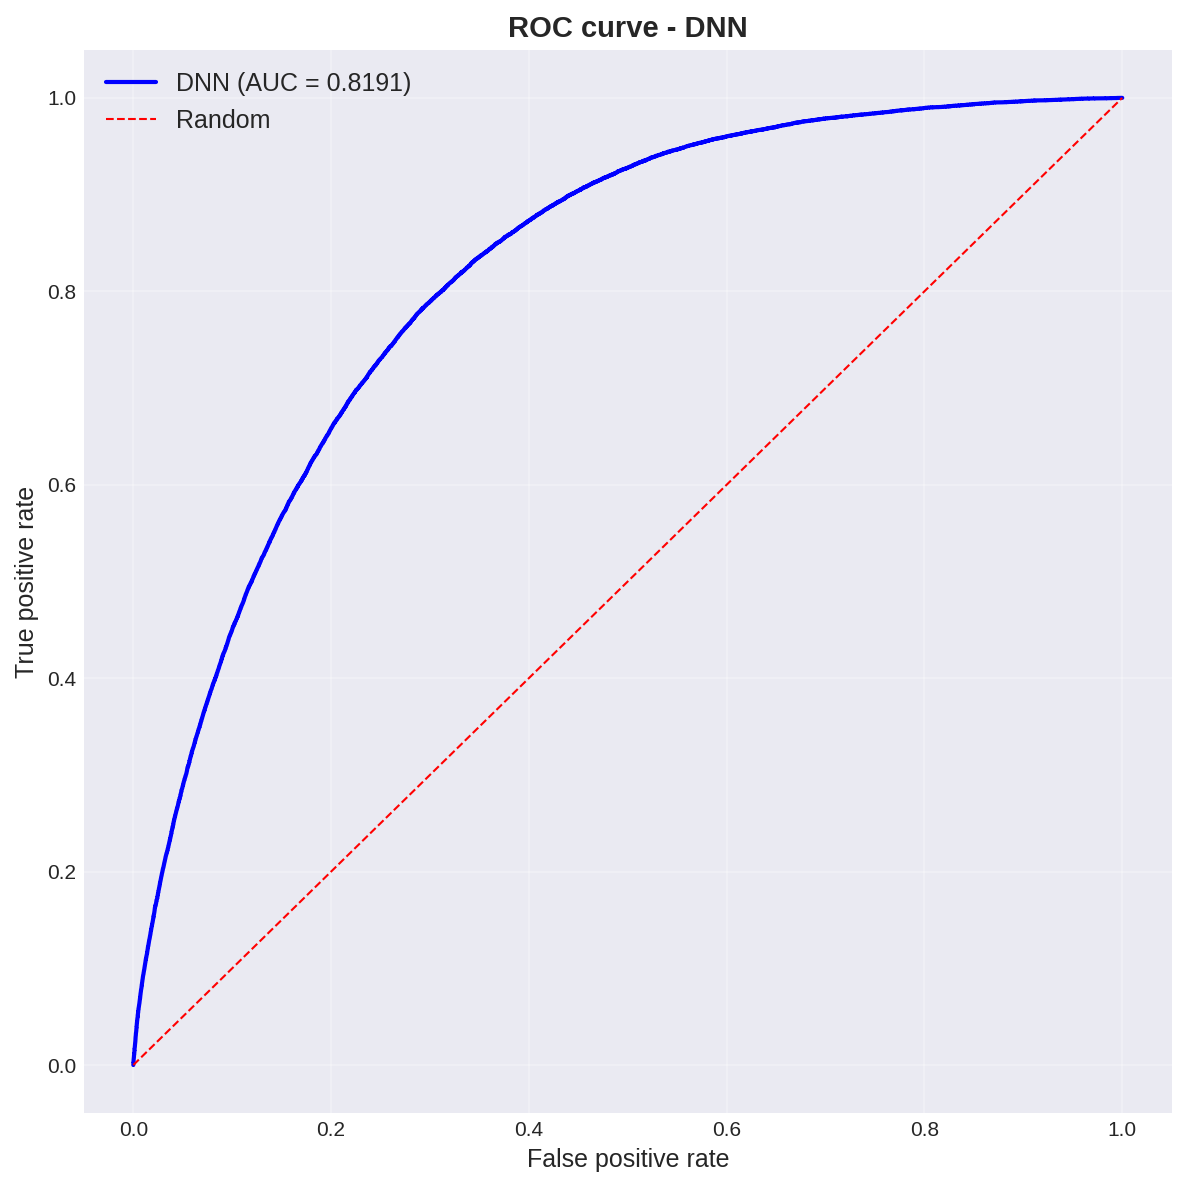
\includegraphics[width=\textwidth]{figures/dnn_roc_curve.png}
        \caption{Courbe ROC du DNN (AUC = 0,819)}
        \label{fig:dnn_roc}
    \end{subfigure}
    \hfill
    \begin{subfigure}[b]{0.48\textwidth}
        \centering
        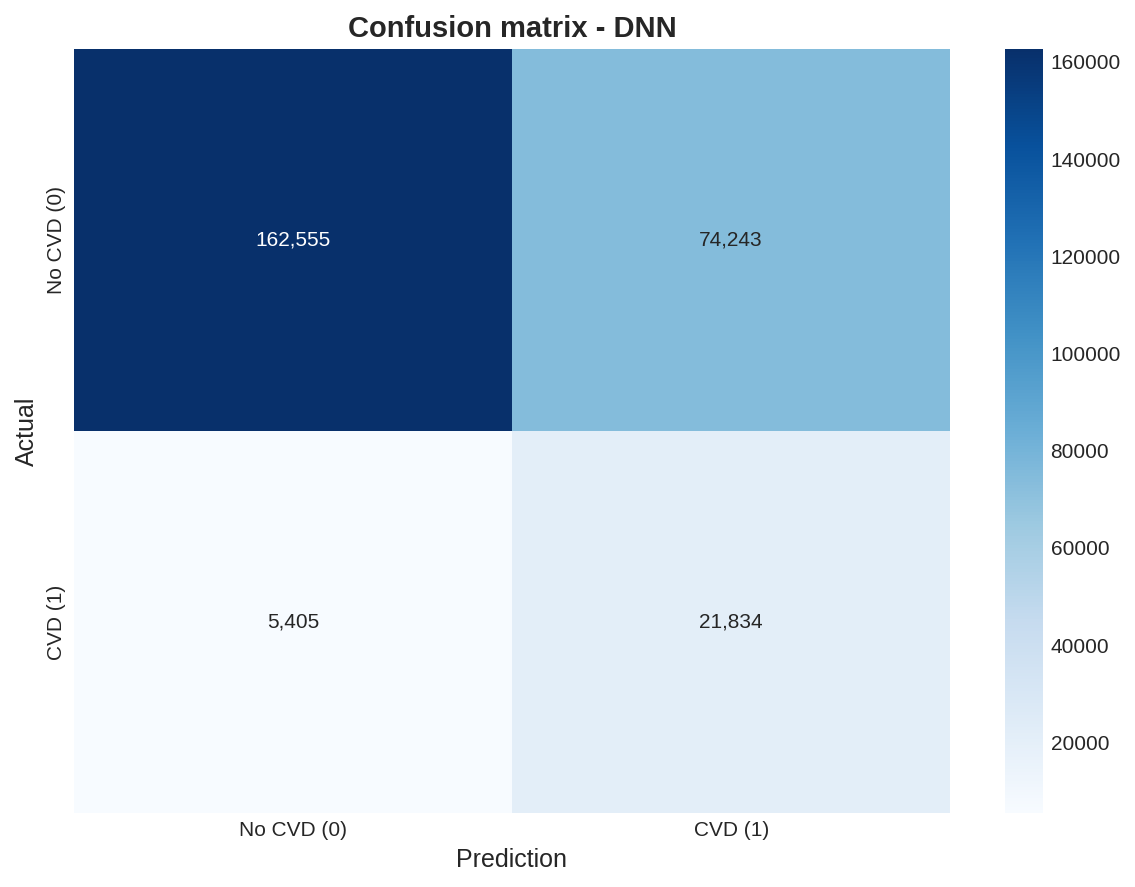
\includegraphics[width=\textwidth]{figures/dnn_confusion_matrix.png}
        \caption{Matrice de confusion (seuil 0,6713)}
        \label{fig:dnn_cm}
    \end{subfigure}
    \caption{Résultats du DNN~: courbe ROC et matrice de confusion au seuil optimal.
             15\,333 vrais positifs (patients MCV correctement identifiés)
             contre 11\,906 faux négatifs.}
    \label{fig:dnn_results}
\end{figure}

\subsection{Résultats détaillés d'XGBoost}

La figure~\ref{fig:xgb_results} présente la courbe ROC et la matrice de confusion
d'XGBoost au seuil par défaut 0,5.

\begin{figure}[H]
    \centering
    \begin{subfigure}[b]{0.48\textwidth}
        \centering
        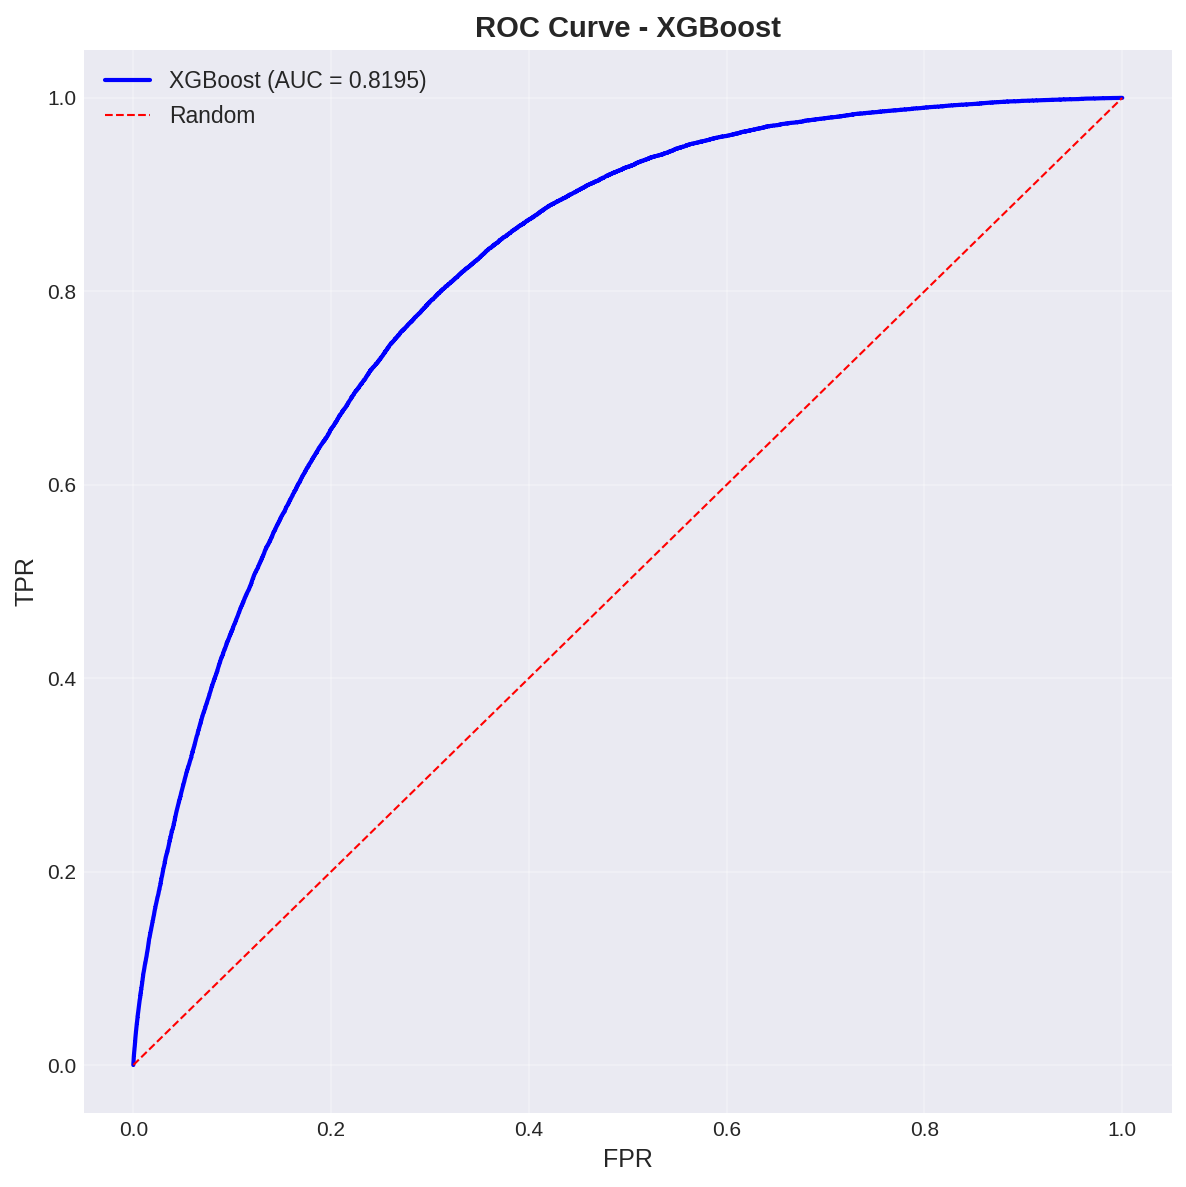
\includegraphics[width=\textwidth]{figures/xgboost_roc_curve.png}
        \caption{Courbe ROC XGBoost (AUC = 0,820)}
        \label{fig:xgb_roc}
    \end{subfigure}
    \hfill
    \begin{subfigure}[b]{0.48\textwidth}
        \centering
        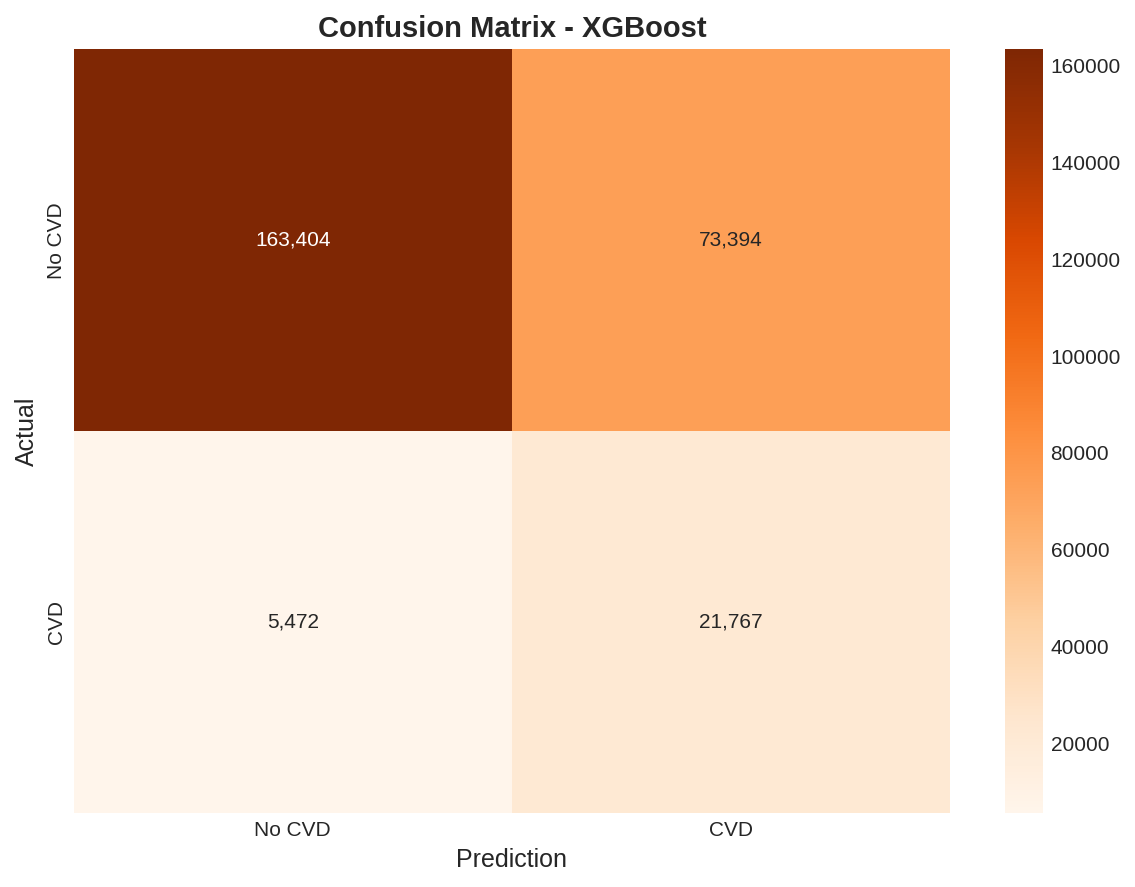
\includegraphics[width=\textwidth]{figures/xgboost_confusion_matrix.png}
        \caption{Matrice de confusion (seuil 0,5)}
        \label{fig:xgb_cm}
    \end{subfigure}
    \caption{Résultats XGBoost~: courbe ROC et matrice de confusion au seuil 0,5.
             21\,767 vrais positifs contre 5\,472 faux négatifs~; le rappel
             plus élevé (79,9\%) se fait au prix de 73\,394 faux positifs.}
    \label{fig:xgb_results}
\end{figure}

\subsection{Comparaison des courbes ROC}

La figure~\ref{fig:roc} superpose les courbes ROC des trois modèles.

\begin{figure}[H]
    \centering
    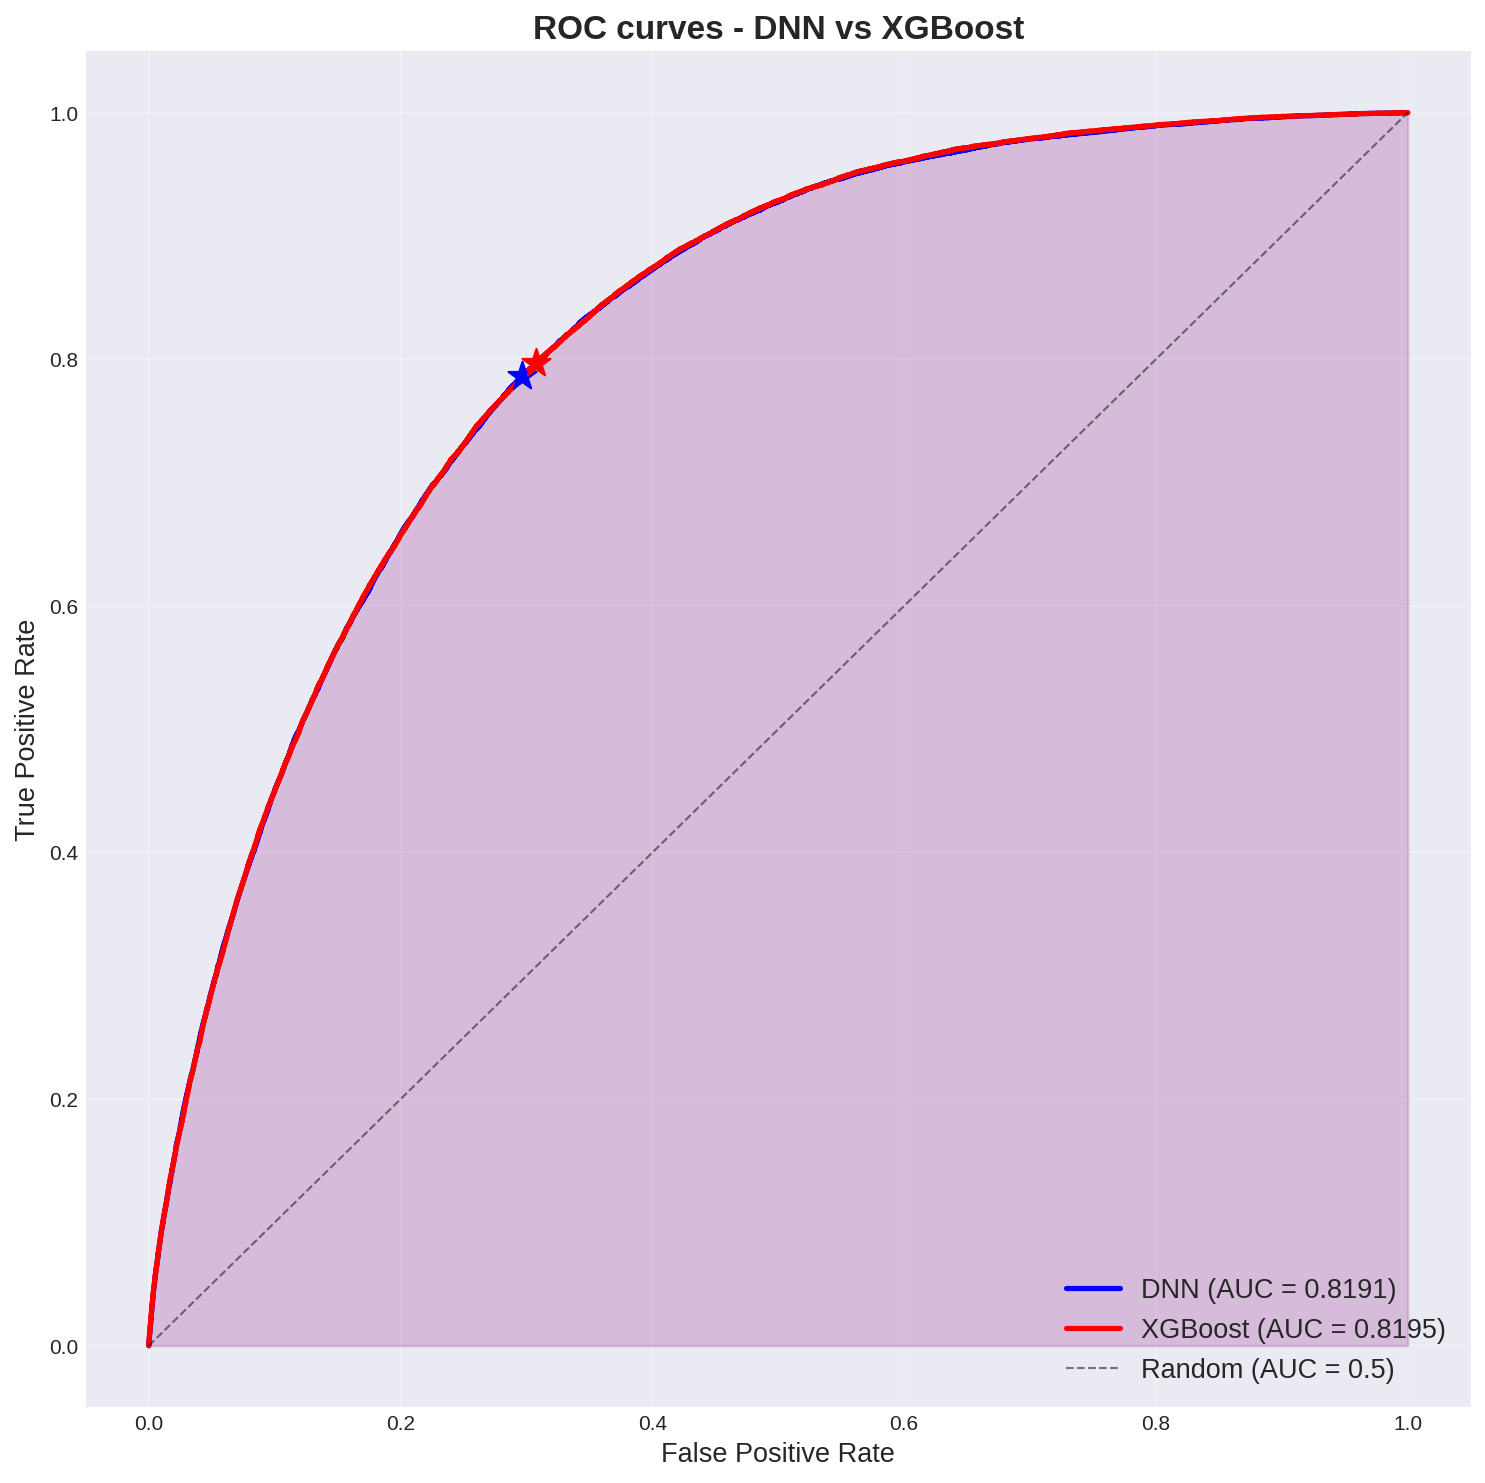
\includegraphics[width=0.85\textwidth]{figures/roc_curves.png}
    \caption{Courbes ROC superposées — DNN, XGBoost et Spark GBT. Les trois modèles
             convergent remarquablement vers le même AUC d'environ 0,82, indiquant
             un plateau déterminé par l'information disponible dans les features
             et non par les architectures des modèles.}
    \label{fig:roc}
\end{figure}

La convergence vers un AUC commun de 0,82 pour trois architectures fondamentalement
différentes (réseau de neurones profond, boosting de gradient, GBT distribué)
constitue une observation forte~: la limite de performance est imposée par
les données disponibles, et notamment par l'absence de \texttt{HighBP} et
\texttt{HighChol}, les deux variables les plus discriminantes selon la littérature.

\subsection{Matrices de confusion comparatives}

\begin{figure}[H]
    \centering
    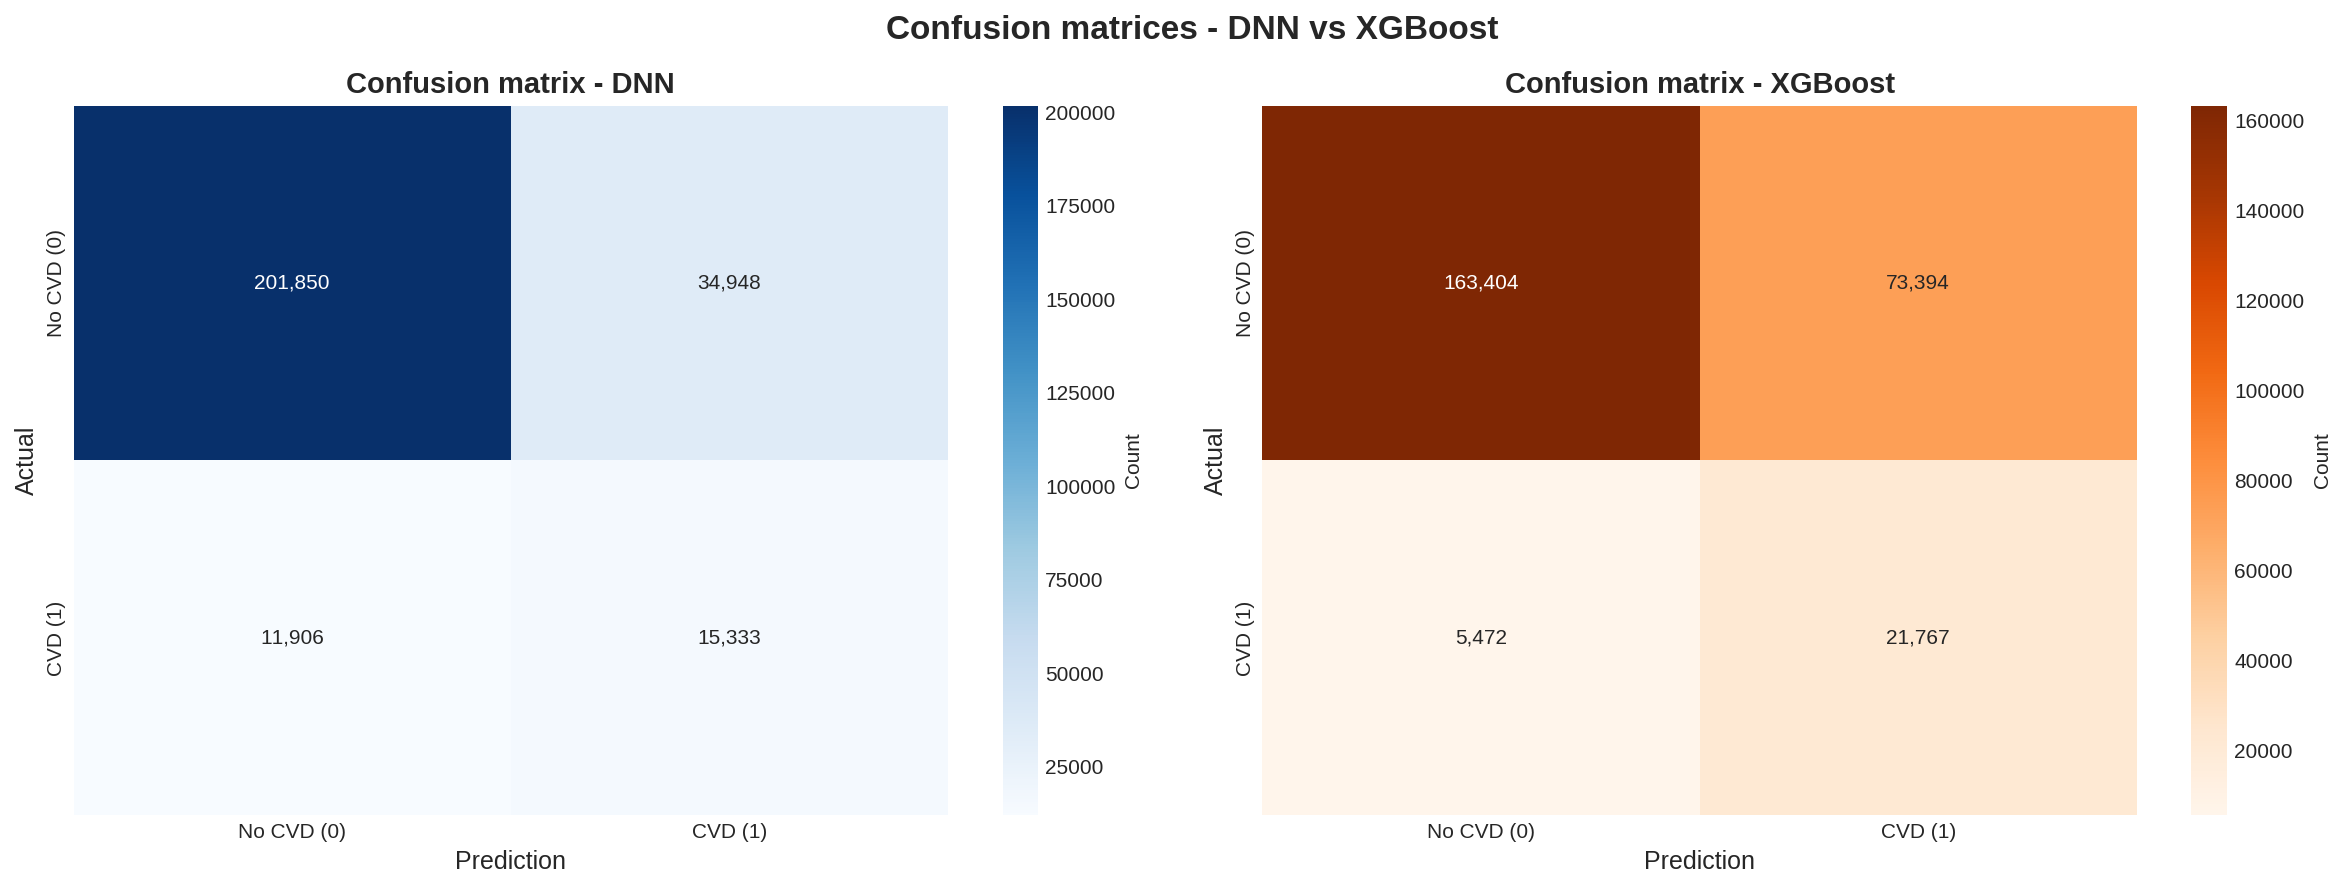
\includegraphics[width=\textwidth]{figures/confusion_matrices.png}
    \caption{Matrices de confusion comparatives — DNN (seuil 0,6713) et XGBoost
             (seuil 0,5). XGBoost présente moins de faux négatifs (5\,472 vs.
             11\,906) mais beaucoup plus de faux positifs (73\,394 vs. 34\,948).}
    \label{fig:cm}
\end{figure}

\begin{table}[H]
\centering
\caption{Analyse des matrices de confusion (jeu de test, 264\,037 observations)}
\label{tab:cm_analysis}
\begin{tabular}{lcccc}
\toprule
\textbf{Modèle} & \textbf{VP} & \textbf{FP} & \textbf{VN} & \textbf{FN} \\
\midrule
DNN (seuil 0,6713) & 15\,333 & 34\,948 & 201\,850 & 11\,906 \\
XGBoost (seuil 0,5) & 21\,767 & 73\,394 & 163\,404 &  5\,472 \\
\bottomrule
\end{tabular}
\end{table}

L'interprétation clinique de ce compromis est essentielle~:
\begin{itemize}
    \item \textbf{XGBoost} (rappel = 79,9\%)~: outil de dépistage précoce privilégiant
          la sensibilité — moins de patients MCV manqués, au prix d'un plus grand
          nombre de faux positifs nécessitant des examens complémentaires.
    \item \textbf{DNN (seuil 0,67)} (rappel = 56,3\%, précision = 30,5\%)~:
          outil de confirmation, réduisant les fausses alertes au détriment d'une
          plus grande proportion de MCV non détectées.
\end{itemize}

\subsection{Courbes d'apprentissage du DNN}

\begin{figure}[H]
    \centering
    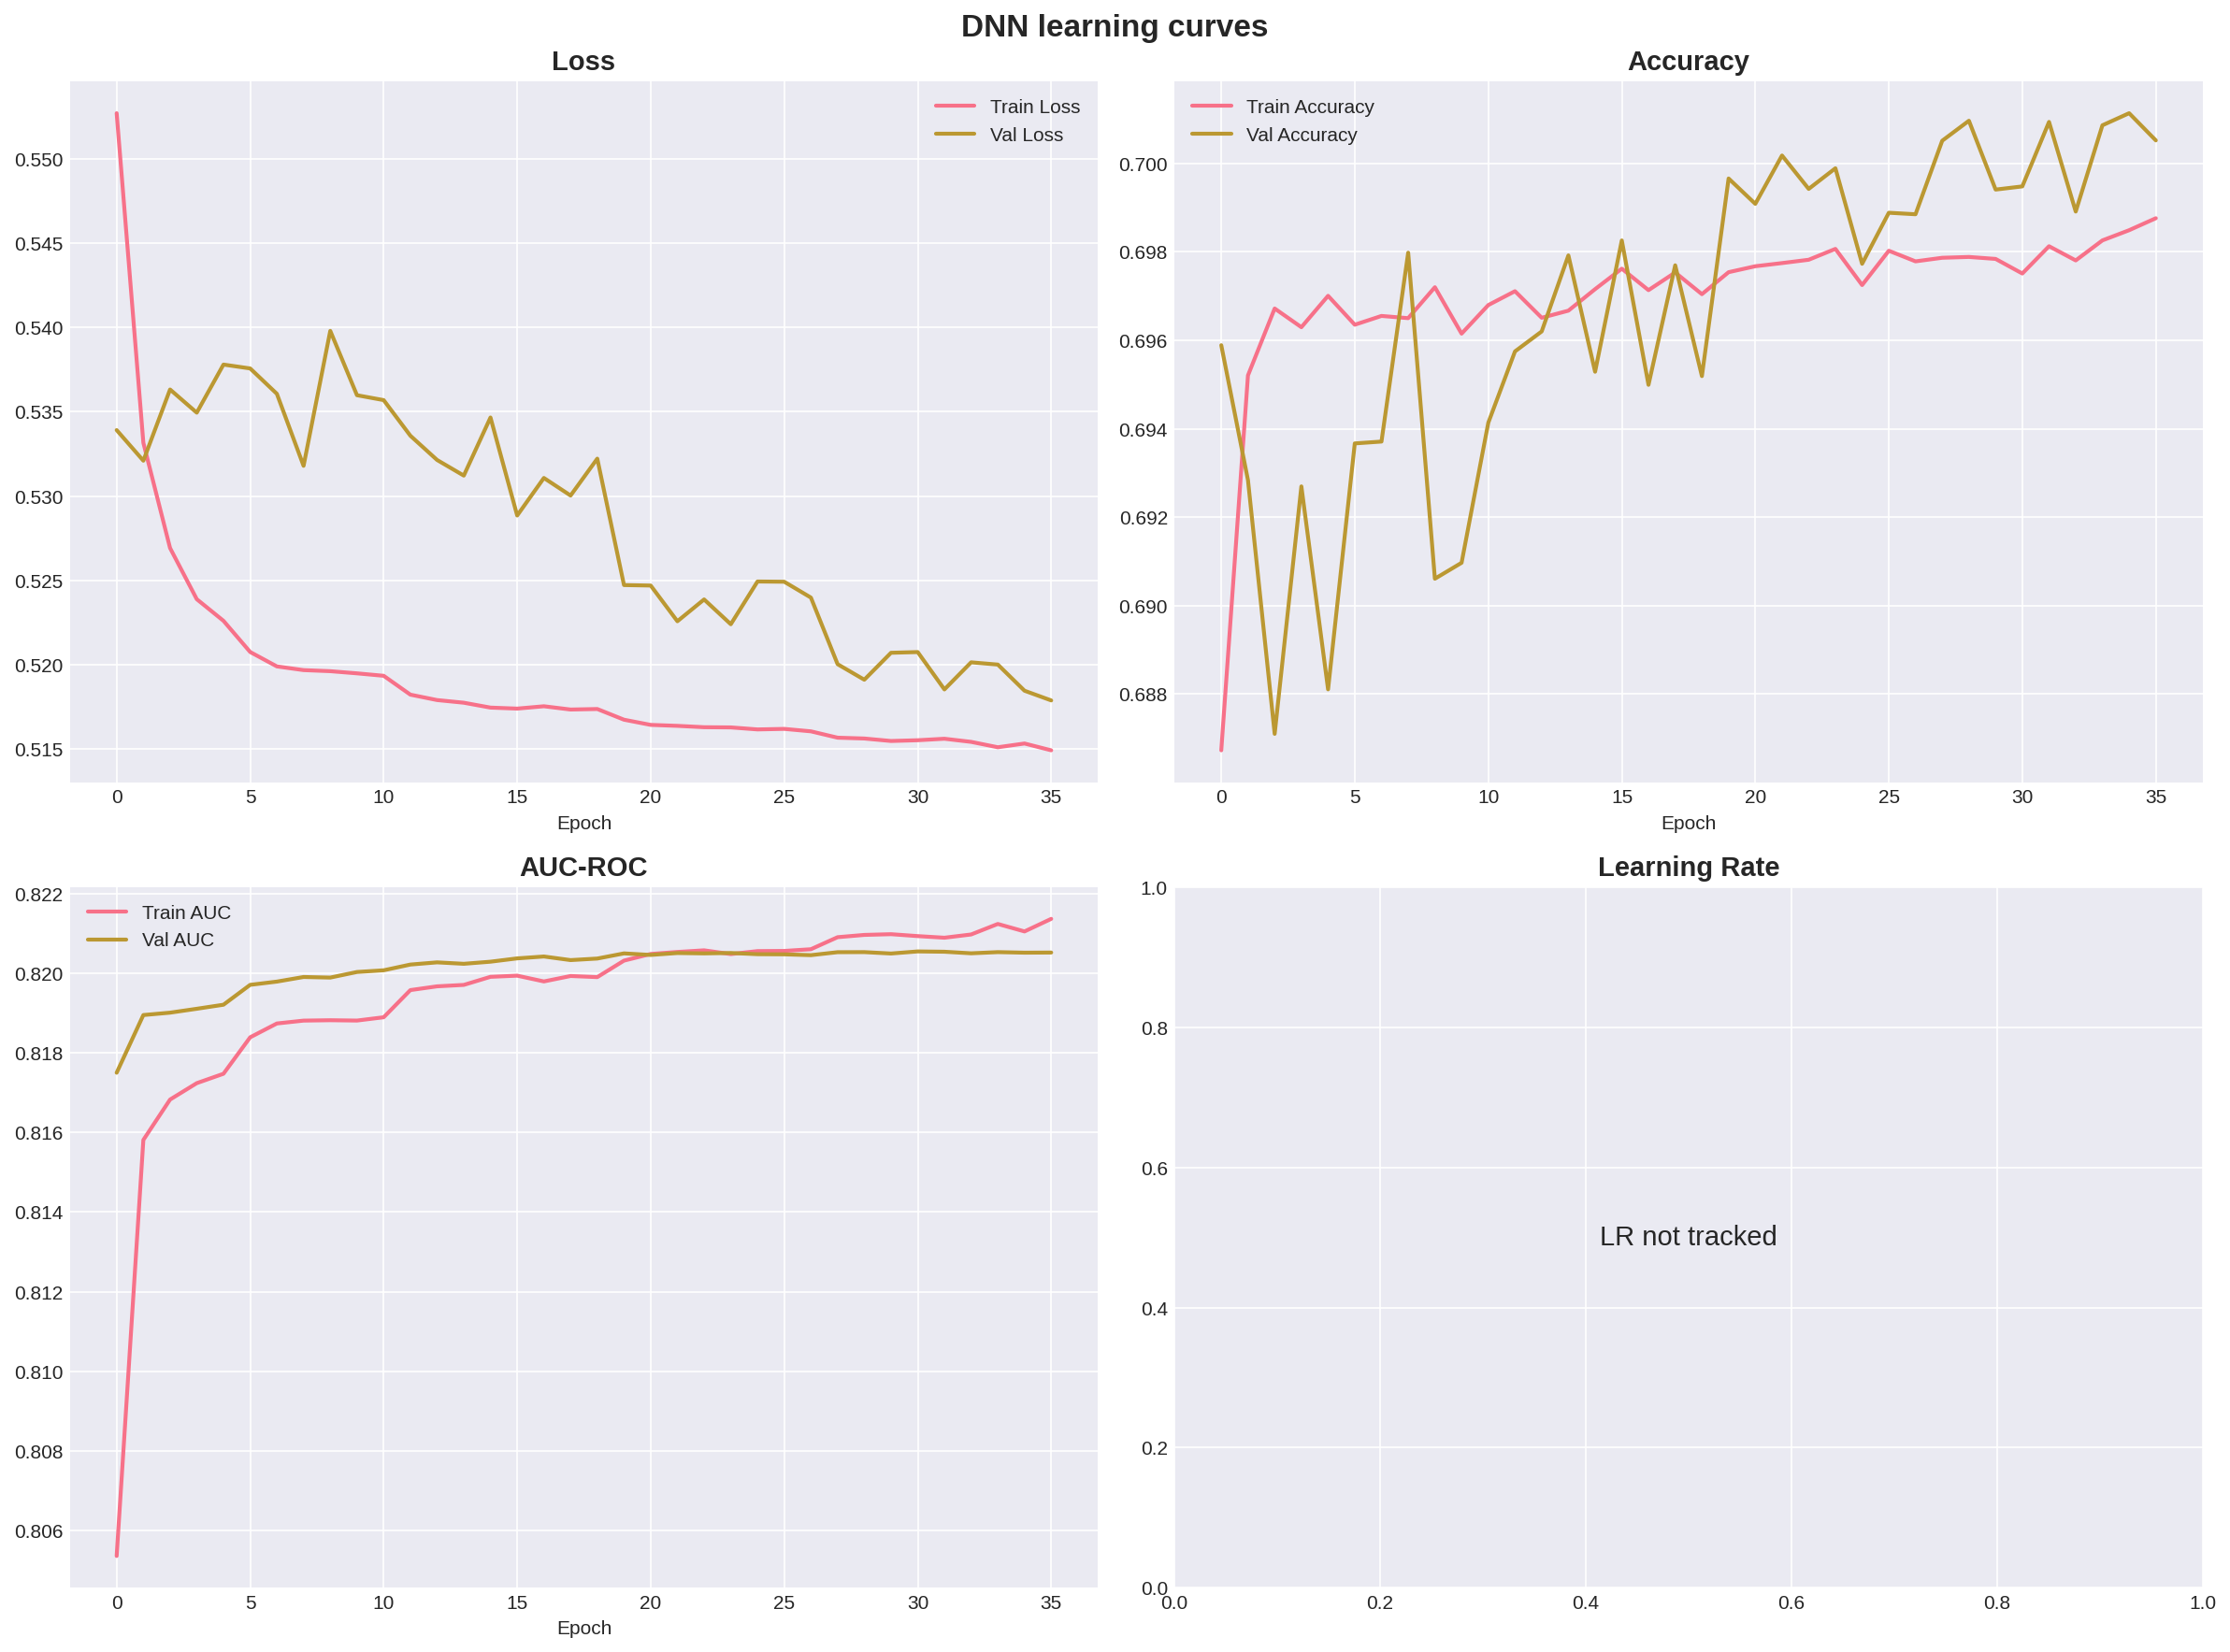
\includegraphics[width=0.85\textwidth]{figures/dnn_learning_curves.png}
    \caption{Courbes d'apprentissage du DNN — perte (gauche) et AUC (droite)
             sur les ensembles d'entraînement et de validation.
             L'AUC dépasse 0,82 dès l'epoch~1 et évolue faiblement
             (+0,003 sur 36 epochs), confirmant que le plateau est inhérent
             aux données et non à une capacité insuffisante du modèle.}
    \label{fig:lc}
\end{figure}

La convergence rapide et parallèle des courbes d'entraînement et de validation
(absence d'écart significatif) confirme l'absence de surapprentissage.
La combinaison Dropout (taux 0,30), BatchNormalization et régularisation $L_2$
($\lambda = 10^{-4}$) est efficace pour un jeu d'entraînement de 1,2~million
d'observations.

\subsection{Analyse du seuil de classification DNN}

\begin{figure}[H]
    \centering
    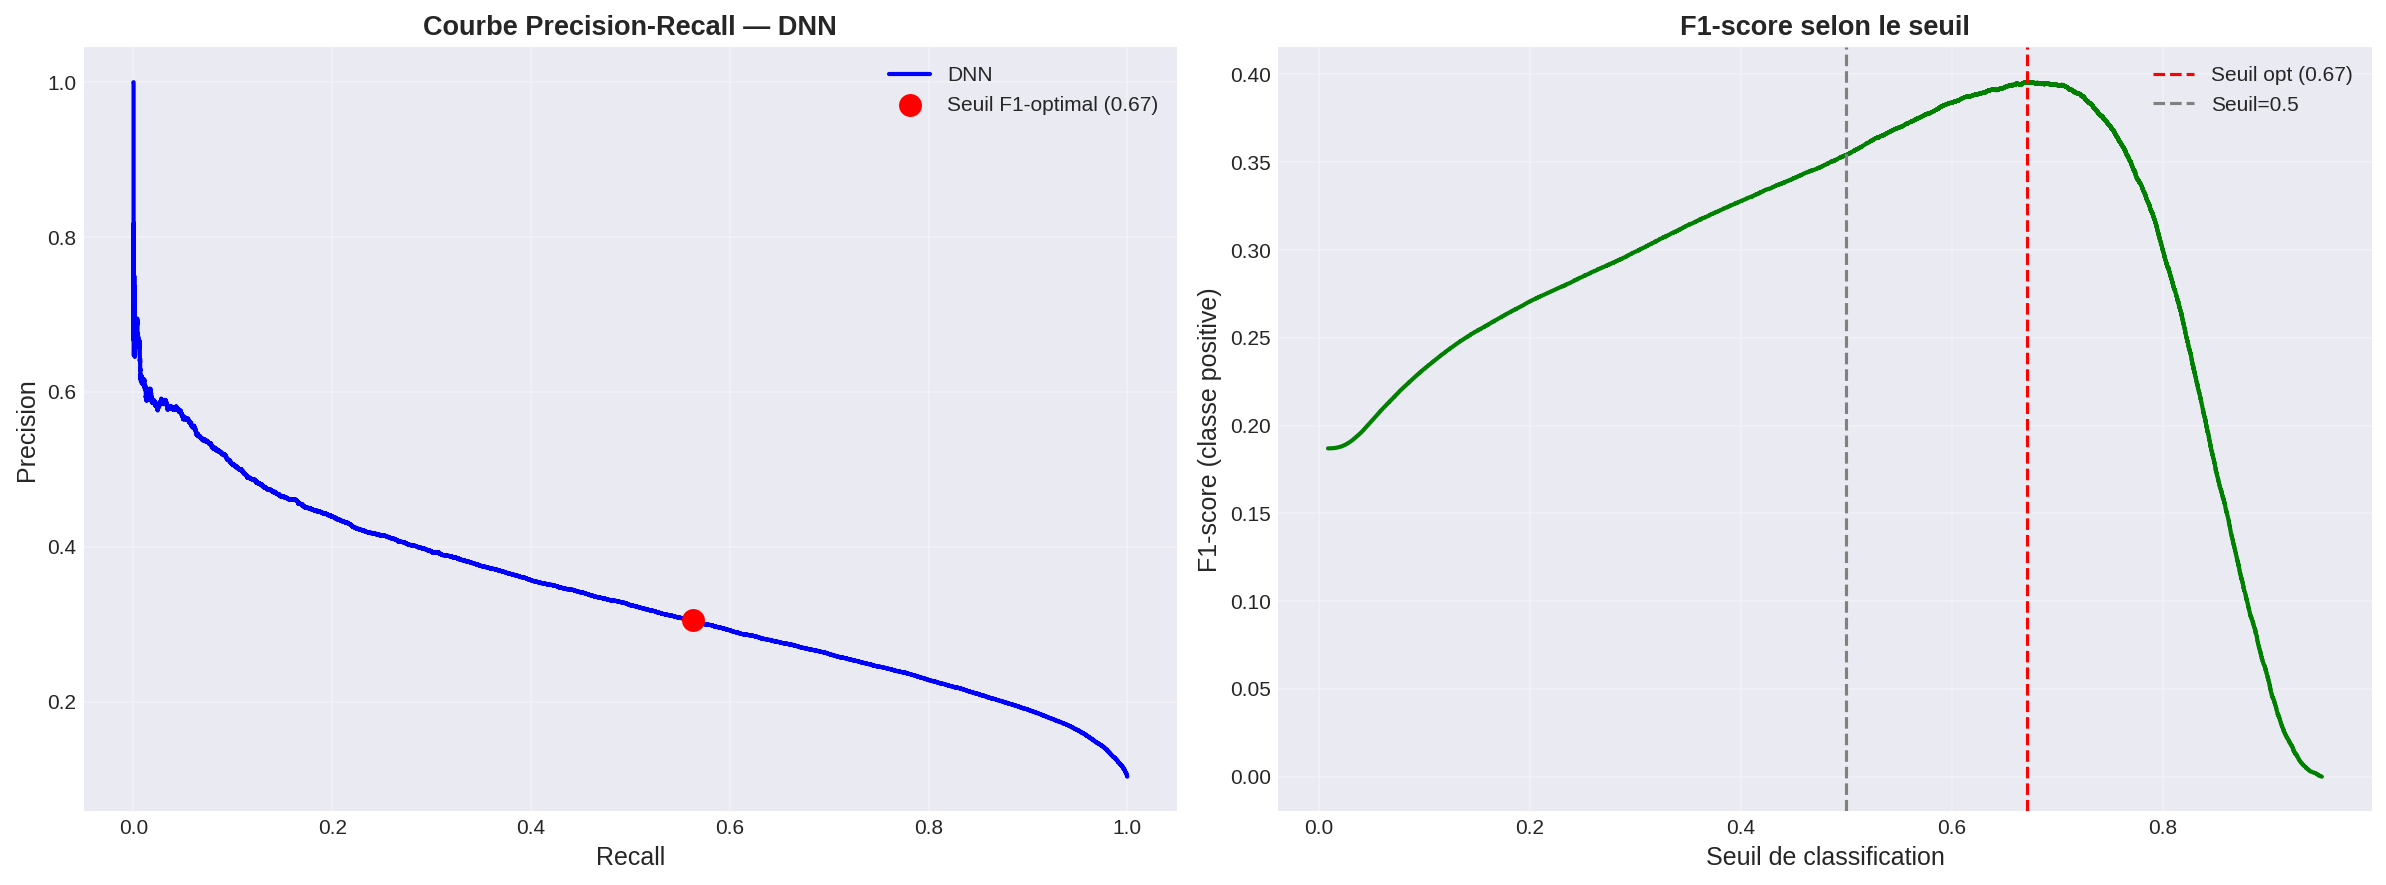
\includegraphics[width=0.85\textwidth]{figures/dnn_threshold_analysis.png}
    \caption{Courbe Précision-Rappel et F1-Score en fonction du seuil de
             classification. Le seuil optimal $\tau^* = 0{,}6713$ maximise le
             F1-score à 0,396. Le seuil par défaut 0,5 produit un rappel élevé
             (0,80) mais une précision très faible (0,23).}
    \label{fig:threshold}
\end{figure}

\begin{table}[H]
\centering
\caption{Impact du seuil de classification sur les métriques du DNN}
\label{tab:threshold_impact}
\begin{tabular}{lccc}
\toprule
\textbf{Seuil} & \textbf{Accuracy} & \textbf{Rappel} & \textbf{F1} \\
\midrule
0,50 (par défaut)       & 0,698 & 0,802 & 0,354 \\
0,6713 (F1-optimal) & 0,822 & 0,563 & 0,396 \\
\midrule
Gain relatif & +17,7\% & $-$29,8\% & +11,9\% \\
\bottomrule
\end{tabular}
\end{table}

L'optimisation du seuil améliore le F1-score de 11,9\% en acceptant une réduction
de 29,8\% du rappel. Ce compromis met en évidence l'importance du choix du seuil
dans les applications cliniques : il n'existe pas de seuil universellement optimal,
et la décision doit être guidée par les coûts relatifs des faux positifs et des
faux négatifs dans le contexte clinique visé.

\subsection{Importance des features XGBoost}

\begin{figure}[H]
    \centering
    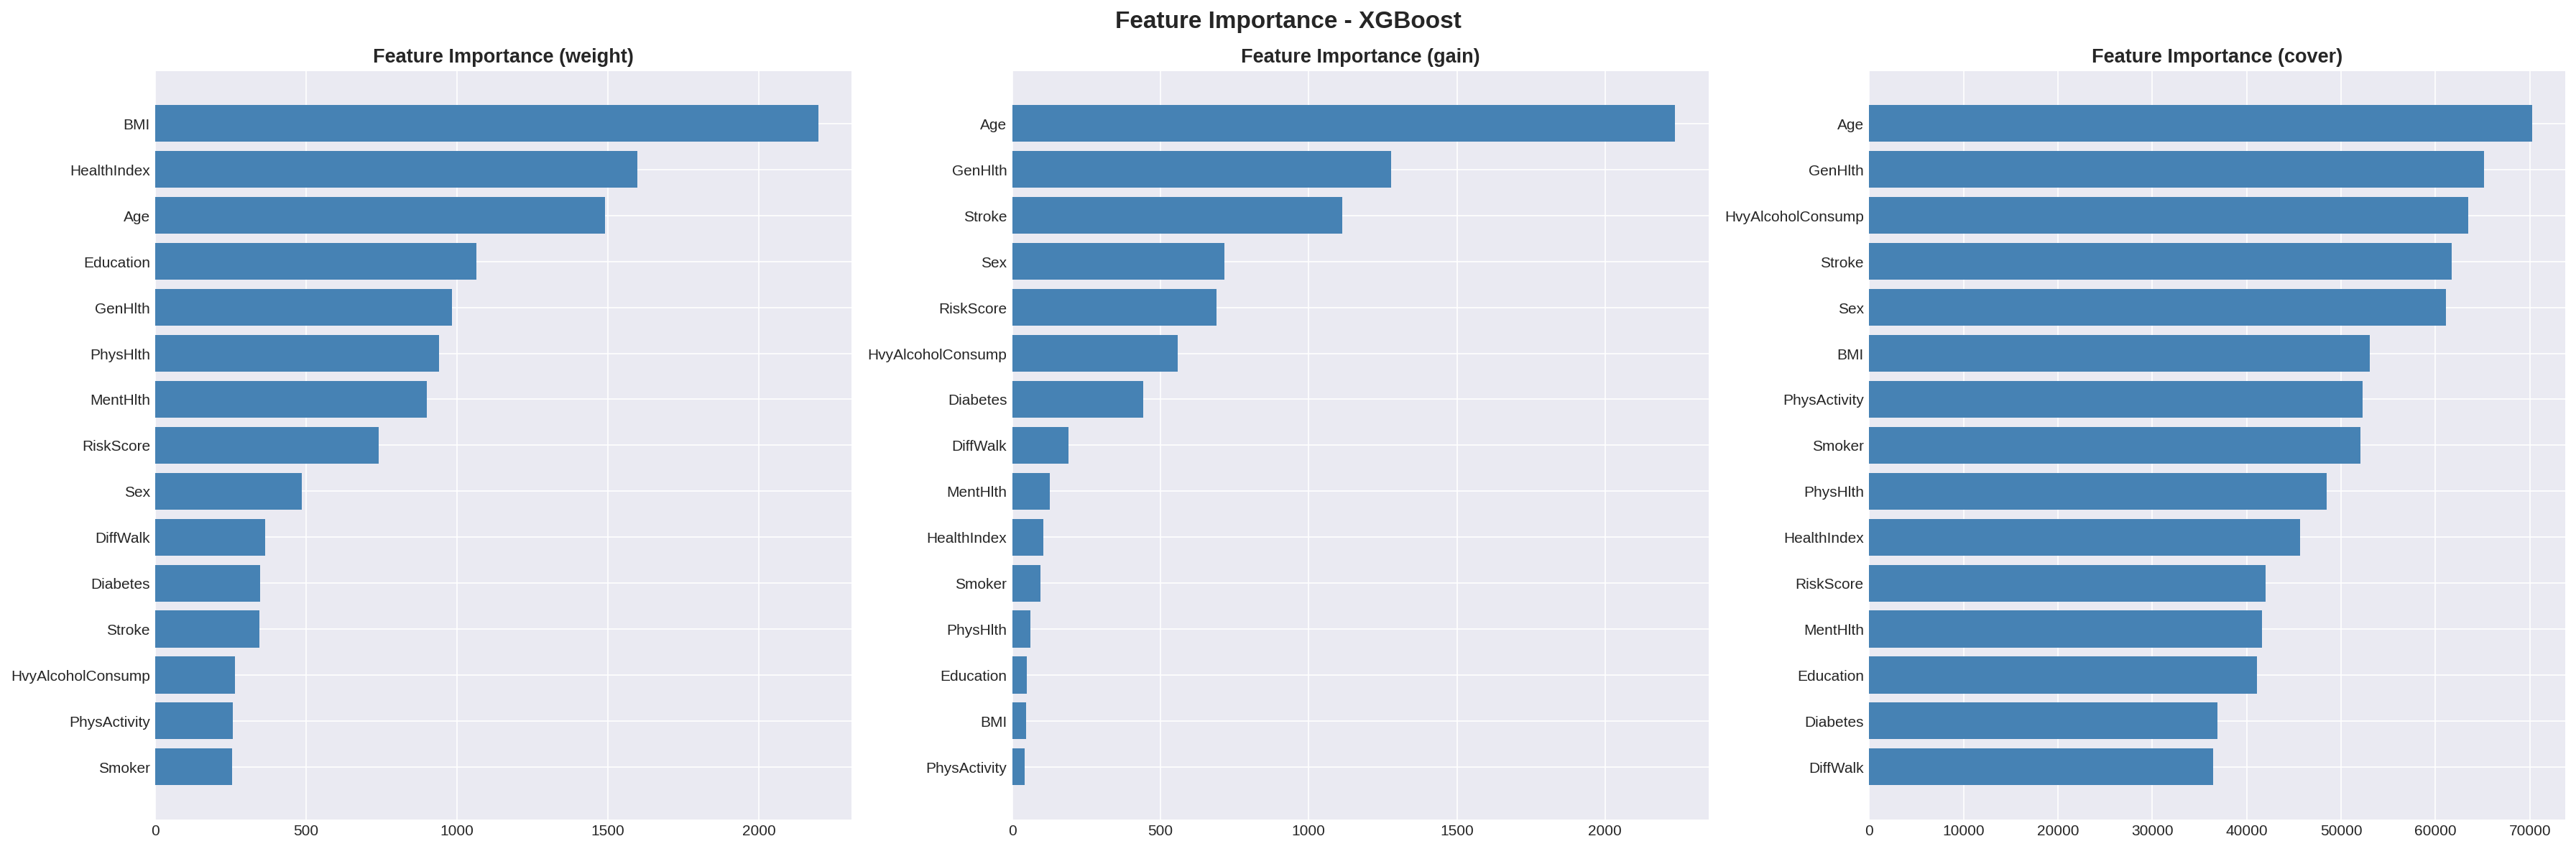
\includegraphics[width=0.85\textwidth]{figures/xgboost_feature_importance.png}
    \caption{Importance des features XGBoost selon trois critères~:
             \textit{weight} (fréquence de coupure), \textit{gain}
             (gain d'information moyen par coupure) et \textit{cover}
             (fraction d'observations affectées). Le critère \textit{gain}
             est le plus informatif~: Age, GenHlth et Stroke dominent,
             en concordance avec l'importance Gini du Random Forest préliminaire.}
    \label{fig:xgb_fi}
\end{figure}

Le critère \textit{weight} place BMI en tête~: sa grande plage de valeurs distinctes
(variable continue) génère naturellement un plus grand nombre de points de coupure
utilisés, sans que cela reflète une importance prédictive supérieure.
Ce biais de fréquence, bien documenté pour les variables continues dans XGBoost,
explique la divergence avec le critère \textit{gain}, qui reste la référence
pour comparer l'importance effective des features.

% ─────────────────────────────────────────────────────────────────────────────
\section{Impact d'Apache Spark}
% ─────────────────────────────────────────────────────────────────────────────

\subsection{Benchmark temporel Spark vs. XGBoost standalone}

La figure~\ref{fig:benchmark} présente les temps d'entraînement comparatifs
entre XGBoost standalone et Spark GBTClassifier pour cinq fractions croissantes
du jeu de données.

\begin{figure}[H]
    \centering
    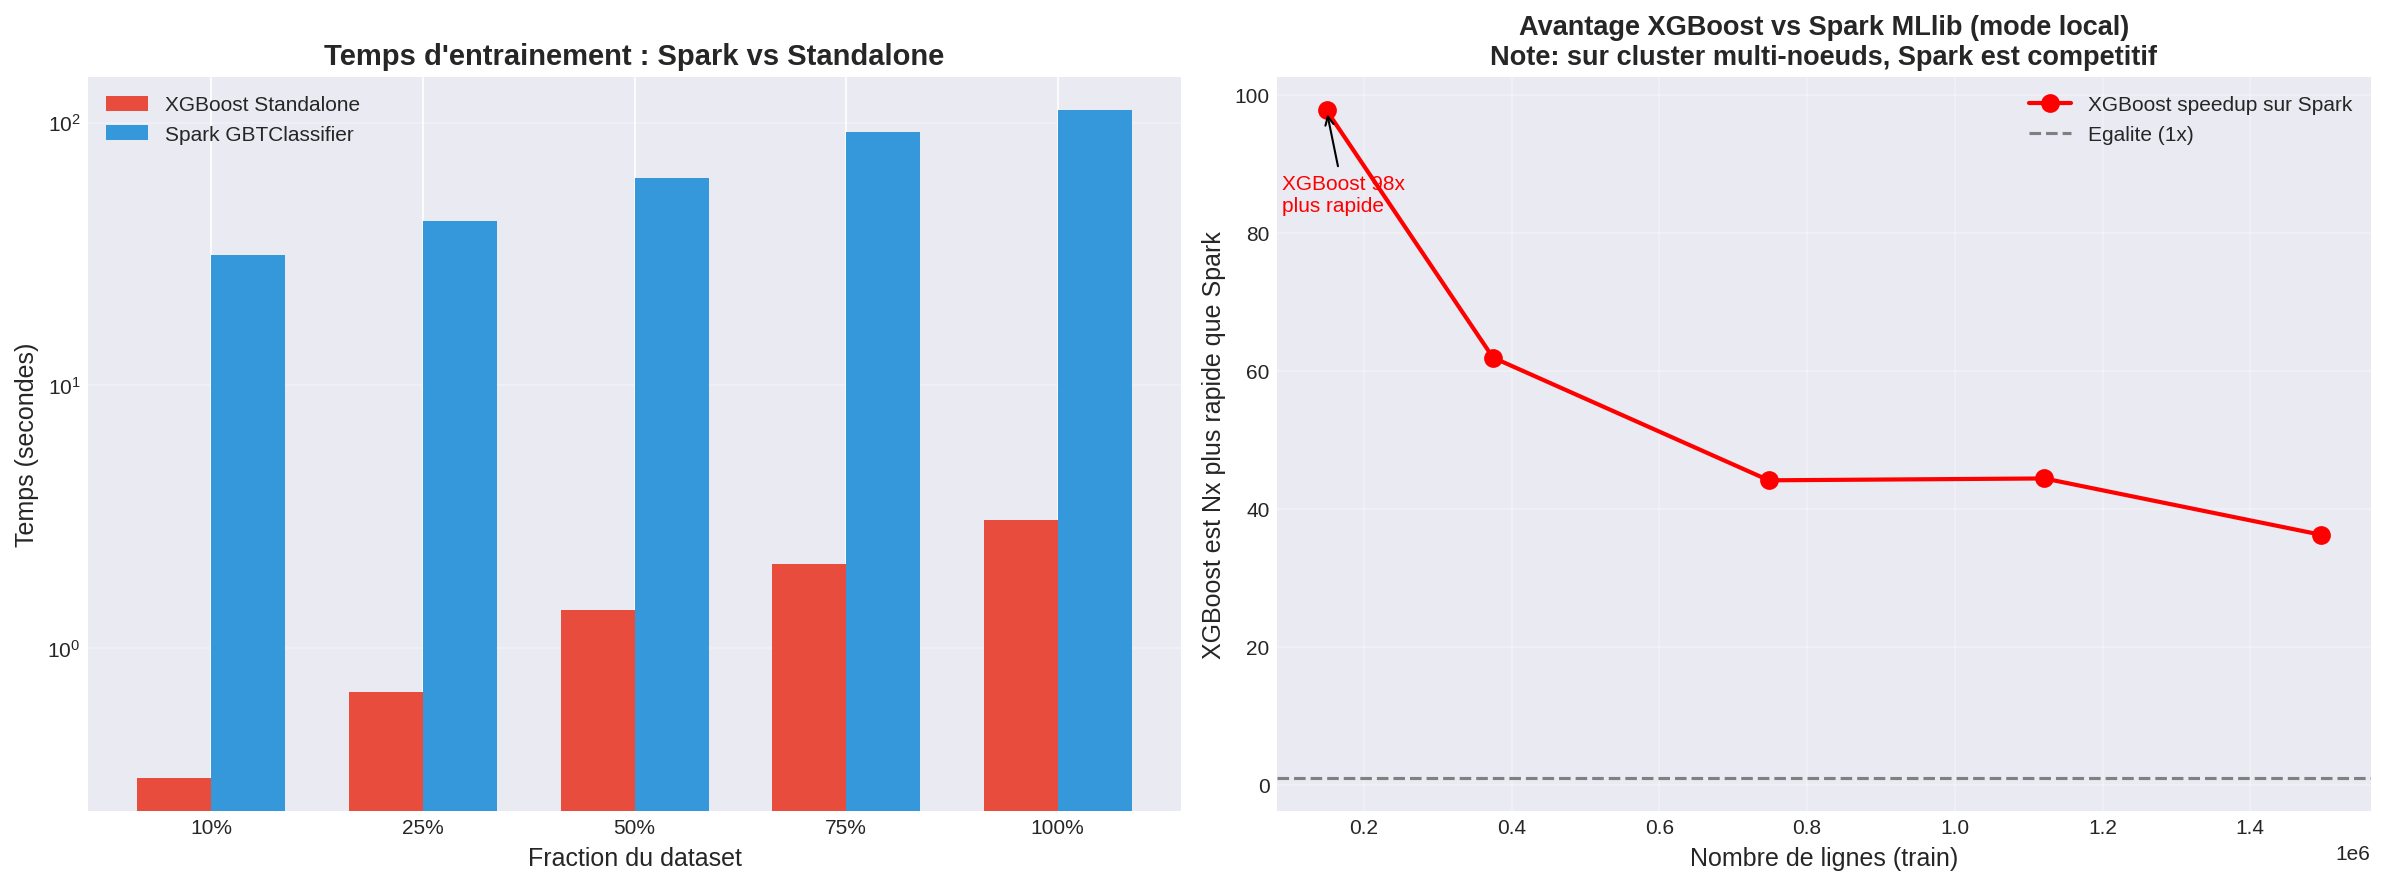
\includegraphics[width=\textwidth]{figures/spark_benchmark_comparison.png}
    \caption{Benchmark temps d'entraînement --- Spark GBT vs XGBoost standalone
             sur cinq fractions du jeu de données (10\% à 100\%).
             L'avantage XGBoost est maximal pour les petits volumes (97,7$\times$
             à 150\,000 lignes) et se réduit à 36$\times$ pour le volume complet.}
    \label{fig:benchmark}
\end{figure}

\begin{table}[H]
\centering
\caption{Résultats détaillés du benchmark (mode local, Kaggle T4 $\times$2)}
\label{tab:benchmark}
\begin{tabular}{lrrrr}
\toprule
\textbf{Fraction} & \textbf{N lignes} & \textbf{Spark GBT (s)} & \textbf{XGBoost (s)} & \textbf{Avantage XGB} \\
\midrule
10\%  &    149\,510 &  31,23 &  0,32 & $\mathbf{97{,}7\times}$ \\
25\%  &    374\,916 &  42,07 &  0,68 & $\mathbf{61{,}9\times}$ \\
50\%  &    748\,199 &  61,41 &  1,39 & $\mathbf{44{,}2\times}$ \\
75\%  &  1\,121\,242 &  92,24 &  2,08 & $\mathbf{44{,}3\times}$ \\
100\% &  1\,495\,609 & 111,35 &  3,07 & $\mathbf{36{,}2\times}$ \\
\bottomrule
\end{tabular}
\end{table}

\subsection{Comparaison globale des temps d'exécution}

La figure~\ref{fig:timing} compare les temps d'entraînement et d'inférence
des trois modèles finaux (DNN, XGBoost avec RandomizedSearchCV, Spark GBT)
dans leur configuration complète.

\begin{figure}[H]
    \centering
    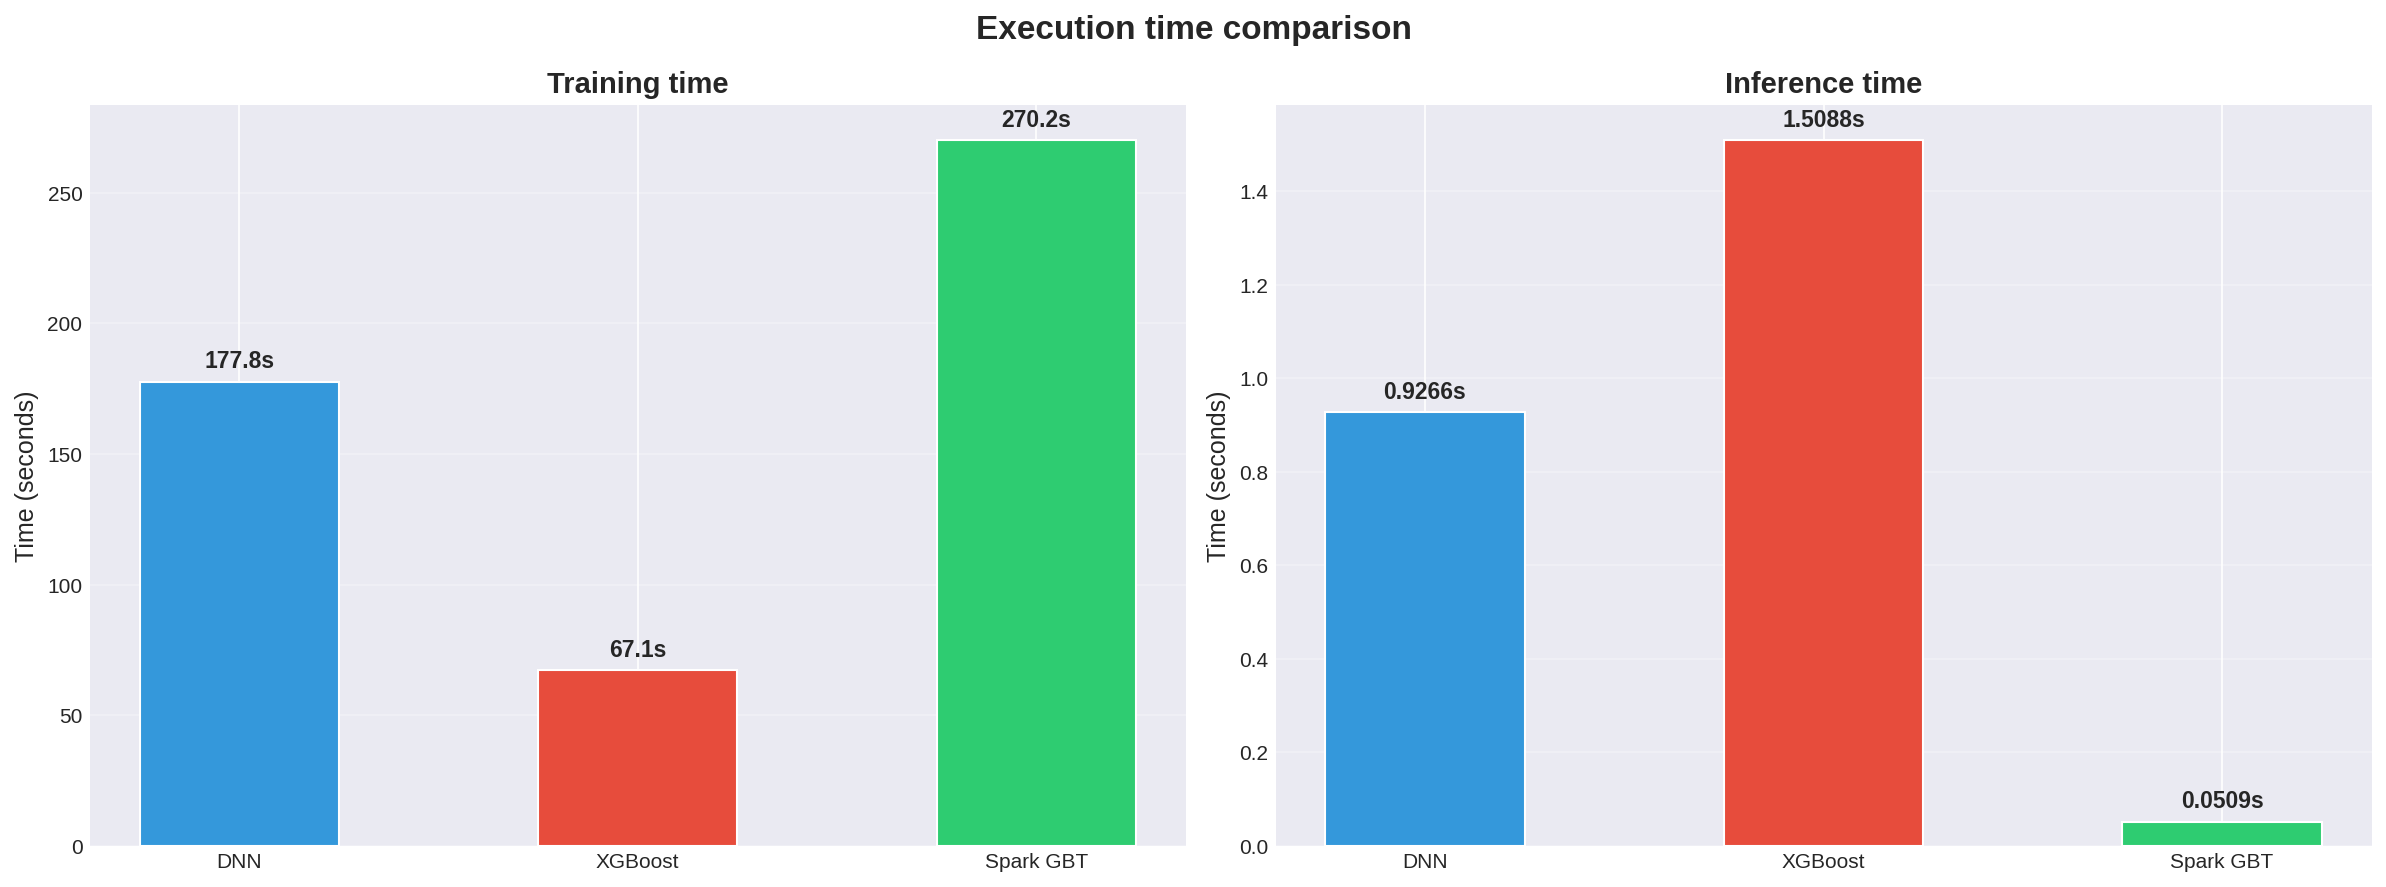
\includegraphics[width=\textwidth]{figures/timing_comparison.png}
    \caption{Comparaison des temps d'entraînement et d'inférence des trois modèles.
             XGBoost (67,1~s d'entraînement, 1,5~s d'inférence) offre le meilleur
             rapport performance/coût computationnel.
             Spark GBT (270,2~s) est le plus lent en mode local~;
             le DNN (177,8~s) bénéficie de l'accélération GPU.}
    \label{fig:timing}
\end{figure}

\textbf{Observations principales~:}
\begin{enumerate}
    \item XGBoost est \textbf{36 à 97 fois plus rapide} que Spark GBT en mode local.
          Cet écart est maximal pour les petits volumes (97,7$\times$ à 150\,000 lignes)
          et se réduit à mesure que le volume augmente, reflétant l'amortissement
          progressif de l'overhead fixe du scheduler Spark.
    \item Le temps Spark croît de façon quasi-linéaire (31~s $\to$ 111~s pour 10$\times$
          plus de données), ce qui traduit l'overhead constant du scheduler par partition.
    \item Le temps XGBoost croît de façon sous-linéaire (0,32~s $\to$ 3,07~s),
          bénéficiant de la parallélisation native C++/CUDA.
\end{enumerate}

\subsection{Apport réel de Spark dans ce pipeline}

Bien que Spark GBTClassifier soit systématiquement plus lent qu'XGBoost en mode
local, Apache Spark apporte une valeur ajoutée indispensable dans les phases de
preprocessing~:

\begin{itemize}
    \item Lecture et déduplication de 2,17~millions de lignes Parquet en quelques
          secondes~; cette opération bloquerait un DataFrame pandas sur 29~Go de RAM.
    \item Calcul parallèle des statistiques descriptives sur l'ensemble du dataset
          distribué.
    \item Scalabilité~: sur un cluster HDFS/YARN de 8~nœuds ou plus, Spark
          deviendrait compétitif pour des volumes dépassant 10~millions de lignes,
          conformément aux résultats de Zhang et al.~\cite{zhang2023}.
\end{itemize}

% ─────────────────────────────────────────────────────────────────────────────
\section{Vérification des critères de succès (PRD)}
% ─────────────────────────────────────────────────────────────────────────────

\begin{table}[H]
\centering
\caption{Vérification des critères de succès du PRD}
\label{tab:prd_check}
\begin{tabular}{llll}
\toprule
\textbf{Critère} & \textbf{Cible PRD} & \textbf{Résultat} & \textbf{Statut} \\
\midrule
AUC-ROC DNN      & $\geq 0{,}85$ & 0,819 & \textcolor{red}{$\times$ Non atteint} \\
AUC-ROC XGBoost  & $\geq 0{,}87$ & 0,820 & \textcolor{red}{$\times$ Non atteint} \\
F1 classe positive & $\geq 0{,}60$ & 0,396 (DNN, seuil opt.) & \textcolor{red}{$\times$ Non atteint} \\
Recall classe positive & $\geq 0{,}65$ & 0,799 (XGBoost) & \textcolor{green!60!black}{$\checkmark$ Atteint} \\
Pipeline Spark fonctionnel & --- & Oui & \textcolor{green!60!black}{$\checkmark$ Atteint} \\
Dashboard Streamlit & --- & Oui & \textcolor{green!60!black}{$\checkmark$ Atteint} \\
\bottomrule
\end{tabular}
\end{table}

\textbf{Analyse des écarts~:} Les cibles AUC de 0,85 (DNN) et 0,87 (XGBoost)
proviennent de la littérature utilisant des datasets BRFSS incluant \texttt{HighBP}
et \texttt{HighChol}, les deux variables les plus discriminantes.
L'absence de ces variables dans notre fichier poolé ML explique structurellement
un écart de 0,03 à 0,05 en AUC. Cette contrainte est d'ordre documentaire~:
avec les mêmes features, les modèles seraient attendus à des performances comparables
à celles de la littérature.

% ─────────────────────────────────────────────────────────────────────────────
\section{Discussion}
\label{sec:discussion}
% ─────────────────────────────────────────────────────────────────────────────

\subsection{Comparaison avec la littérature}

Le tableau~\ref{tab:etat_art_rappel} repositionne les résultats obtenus dans
le panorama des travaux comparables.

\begin{table}[H]
\centering
\caption{Positionnement des résultats dans la littérature}
\label{tab:etat_art_rappel}
\begin{tabular}{p{3.5cm}p{1.5cm}p{3cm}p{1.5cm}p{3.5cm}}
\toprule
\textbf{Auteurs} & \textbf{Année} & \textbf{Méthode} & \textbf{AUC} & \textbf{Particularités} \\
\midrule
Nickels et al.~\cite{nickels2023}    & 2023 & Random Forest       & 0,912 & Avec HighBP/HighChol \\
Mesdaghinia et al.~\cite{mesdaghinia2023} & 2023 & XGBoost + SMOTE & 0,872 & 23 variables \\
Kumar et al.~\cite{kumar2023}        & 2023 & LSTM                & 0,891 & Données longitudinales \\
Patel et al.~\cite{patel2023}        & 2023 & DNN + SMOTE         & 0,834 & F1=0,834 \\
\midrule
\textbf{Ce travail}                  & 2026 & DNN + XGBoost + Spark & 0,820 & Sans HighBP/HighChol \\
\bottomrule
\end{tabular}
\end{table}

Notre AUC de 0,819--0,820 se positionne de façon cohérente dans la littérature,
compte tenu des contraintes de features. Sans \texttt{HighBP} et \texttt{HighChol},
les performances typiques des travaux BRFSS se situent entre 0,80 et 0,85~;
notre résultat est donc proche de la limite supérieure atteignable avec le jeu
de données disponible.

\subsection{Convergence des modèles}

La convergence remarquable des trois modèles vers le même AUC de 0,82 représente
un résultat théoriquement significatif~: elle suggère l'existence d'un plafond
informationnel déterminé par les features disponibles, indépendamment de
l'architecture du classifieur. Ce phénomène est cohérent avec la théorie de
l'information~: lorsque les features ne contiennent pas suffisamment d'information
pour discriminer les classes, aucune architecture ne peut compenser ce déficit.

\subsection{Gestion du déséquilibre de classes}

La stratégie de pondération de classes s'avère efficace~: le Recall de la classe
positive atteint 79,9\% pour XGBoost (seuil 0,5), ce qui est cliniquement
satisfaisant pour un outil de dépistage précoce. Par rapport à SMOTE \cite{chawla2002smote},
la pondération préserve les distributions statistiques originales, essentielles
pour l'interprétabilité épidémiologique des résultats.

\subsection{Limites de l'étude}

\begin{enumerate}
    \item \textbf{Features manquantes}~: \texttt{HighBP}, \texttt{HighChol},
          \texttt{Income} et \texttt{NoDocbcCost} sont absentes du fichier poolé ML
          disponible, plafonnant la performance maximale atteignable à environ 0,82 en AUC.

    \item \textbf{Mode local Spark}~: L'évaluation de Spark en mode local (une seule
          machine) sous-estime son potentiel réel sur un cluster distribué~; les
          conclusions du benchmark ne sont pas directement généralisables à des
          infrastructures de production multi-nœuds.

    \item \textbf{Nature transversale des données}~: le BRFSS est une enquête
          transversale (une observation par répondant par année). L'absence de
          dimension longitudinale empêche la modélisation de l'évolution temporelle
          des facteurs de risque.

    \item \textbf{Biais de déclaration}~: les données BRFSS étant auto-rapportées,
          elles sont susceptibles de biais de mémorisation et de désirabilité
          sociale, notamment pour les variables comportementales (alcool, tabac,
          activité physique).

    \item \textbf{Métriques Spark}~: la métrique F1 pondérée de Spark (0,860) n'est
          pas comparable aux F1 binaires de la classe positive, en raison du
          déséquilibre de classes et de l'absence de support pour les class weights
          dans le GBTClassifier de Spark MLlib.
\end{enumerate}

\chapter{Conclusion et Perspectives}

\section{Synthèse des travaux}

Ce mémoire décrit un pipeline Big Data pour la prédiction des maladies cardiovasculaires
à partir du dataset BRFSS 2020--2024.
Le pipeline combine Apache Spark pour le traitement des 2,17 millions d'enregistrements
et deux modèles d'apprentissage automatique, un réseau de neurones profond (DNN)
et XGBoost, comparés sur un protocole d'évaluation unifié.

\subsection{Contributions principales}

\begin{enumerate}
    \item \textbf{Pipeline de binarisation BRFSS :} Un pipeline de transformation spécifique au format BRFSS a été développé, gérant les encodages non standards (1=Oui/2=Non), la variable dérivée \texttt{\_MICHD} pour la cible cardiovasculaire composite, et les cas particuliers de chaque variable (valeurs 88, 7, 9 indiquant des données manquantes ou des refus).

    \item \textbf{Traitement distribué à grande échelle :} Apache Spark a permis l'ingestion et le nettoyage de 2,17 millions d'enregistrements Parquet, incluant la suppression de 416\,535 doublons (19,1\% du dataset brut), avec un calcul distribué de statistiques descriptives.

    \item \textbf{Modèles comparatifs :} Deux modèles ont été entraînés et comparés sur le même jeu de test standardisé :
    \begin{itemize}
        \item DNN (256-128-64, 36 epochs, seuil optimal 0,6713) : AUC-ROC = 0,8191, Recall = 56,3\%
        \item XGBoost (400 arbres, max\_depth=5, learning\_rate=0,05) : AUC-ROC = 0,8195, Recall = 79,9\%
    \end{itemize}

    \item \textbf{Benchmark Spark vs. XGBoost :} Quantification précise de l'avantage de XGBoost standalone (36 à 97 fois plus rapide que Spark GBT en mode local), permettant de déduire que l'apport de Spark dans ce pipeline réside principalement dans le preprocessing distribué et non dans l'entraînement.

    \item \textbf{Dashboard interactif :} Un tableau de bord Streamlit en 3 pages a été développé, permettant la visualisation interactive des résultats sans nécessiter d'infrastructure Big Data.
\end{enumerate}

\subsection{Réponse à la problématique}

La problématique initiale — comment exploiter des données épidémiologiques massives pour prédire le risque cardiovasculaire en comparant ML classique et Deep Learning — a reçu les réponses suivantes :

\begin{itemize}
    \item Spark traite 2,17 millions de lignes Parquet en quelques secondes et supprime
          416\,535 doublons, opération inaccessible à pandas sans segmentation manuelle.
    \item Les class weights ($w_1 = 4{,}847$ pour le DNN, $\textit{scale\_pos\_weight} = 8{,}69$
          pour XGBoost) gèrent le déséquilibre sans créer de données synthétiques,
          produisant un recall de 79,9~\% sur la classe positive avec XGBoost.
    \item Les deux modèles convergent vers le même AUC (0,820), XGBoost étant
          2,6 fois plus rapide à entraîner (67~s vs 178~s) et offrant un meilleur
          recall à seuil identique.
    \item L'absence de HighBP et HighChol dans le fichier pooled~ML plafonne l'AUC
          à 0,82, en deçà des cibles de 0,85 (DNN) et 0,87 (XGBoost).
          Cette contrainte est d'origine documentaire et non algorithmique.
\end{itemize}

\section{Perspectives d'amélioration}

\subsection{Amélioration des données}

\begin{enumerate}
    \item \textbf{Intégration des features manquantes :} Utiliser le fichier EDA BRFSS (qui contient HighBP et HighChol) pour les phases de modélisation. L'ajout de ces deux variables permettrait d'estimer une amélioration de 0,03 à 0,05 en AUC, selon la littérature.

    \item \textbf{Données longitudinales :} Exploiter la dimension temporelle du BRFSS (répondants suivis sur plusieurs années) pour construire des modèles séquentiels (LSTM, Transformer temporel) capturant l'évolution des facteurs de risque.

    \item \textbf{Sources de données complémentaires :} Enrichir avec des données cliniques (ECG, biologie), génomiques ou d'imagerie pour une modélisation multimodale.
\end{enumerate}

\subsection{Amélioration des modèles}

\begin{enumerate}
    \item \textbf{Explicabilité :} Intégrer SHAP (\textit{SHapley Additive exPlanations}) \cite{lundberg2017} pour l'interprétation des prédictions individuelles, essentielle en contexte médical pour la confiance des cliniciens.

    \item \textbf{Calibration des probabilités :} Appliquer une calibration isotonique ou Platt scaling pour améliorer la qualité des probabilités prédites, permettant une meilleure optimisation du seuil de décision.

    \item \textbf{Ensemble de modèles :} Combiner DNN et XGBoost par stacking ou blending pour potentiellement surpasser les performances individuelles.

    \item \textbf{AutoML :} Utiliser des frameworks comme H2O AutoML ou AutoGluon pour explorer automatiquement un espace d'architectures plus large.
\end{enumerate}

\subsection{Amélioration de l'infrastructure}

\begin{enumerate}
    \item \textbf{Cluster Spark distribué :} Évaluer Spark sur un cluster HDFS/YARN réel (8+ nœuds) pour quantifier le speedup en conditions industrielles. À cette échelle, Spark GBT devient compétitif avec XGBoost standalone pour les volumes dépassant 10M de lignes.

    \item \textbf{Déploiement en production :} Créer une API REST (FastAPI ou Flask) exposant le modèle XGBoost comme service de prédiction en temps réel, intégrable dans un système d'information hospitalier.

    \item \textbf{Monitoring MLOps :} Mettre en place un pipeline MLOps (MLflow, DVC) pour le suivi des expériences, la versioning des modèles et la détection du drift de données au fil du temps.
\end{enumerate}

\subsection{Amélioration du dashboard}

\begin{enumerate}
    \item \textbf{Inférence en temps réel :} Intégrer le modèle XGBoost dans le dashboard pour permettre des prédictions individuelles à partir d'un formulaire de saisie des facteurs de risque.
    \item \textbf{Rapport automatisé :} Générer un rapport PDF automatique récapitulant les résultats d'une session d'exploration EDA.
\end{enumerate}

\section{Conclusion générale}

Ce travail montre qu'un pipeline Big Data pour la prédiction des MCV est réalisable
avec des outils open-source (PySpark, TensorFlow, XGBoost, Streamlit)
sur une infrastructure académique à machine unique.

Les performances obtenues, AUC de 0,82 et recall de 79,9~\% pour XGBoost,
sont cohérentes avec la littérature sur des jeux de données BRFSS de composition
comparable. L'écart avec les cibles du PRD tient à des contraintes de données,
pas à des limitations des algorithmes.

Spark est utile pour le preprocessing à grande échelle, pas pour l'entraînement
en mode local. Sur un cluster distribué, la combinaison Spark (ingestion, nettoyage)
et XGBoost (entraînement) reste une architecture valide pour des volumes de l'ordre
de la dizaine de millions de lignes.

Les perspectives les plus directes sont l'intégration de HighBP et HighChol
depuis le fichier BRFSS EDA, l'ajout d'une couche d'explicabilité SHAP,
et le déploiement du modèle XGBoost comme API de prédiction.


% Bibliographie
\printbibliography[heading=bibintoc, title={Références bibliographiques}]

\end{document}
